\documentclass[twoside]{book}

% Packages required by doxygen
\usepackage{fixltx2e}
\usepackage{calc}
\usepackage{doxygen}
\usepackage[export]{adjustbox} % also loads graphicx
\usepackage{graphicx}
\usepackage[utf8]{inputenc}
\usepackage{makeidx}
\usepackage{multicol}
\usepackage{multirow}
\PassOptionsToPackage{warn}{textcomp}
\usepackage{textcomp}
\usepackage[nointegrals]{wasysym}
\usepackage[table]{xcolor}

% Font selection
\usepackage[T1]{fontenc}
\usepackage[scaled=.90]{helvet}
\usepackage{courier}
\usepackage{amssymb}
\usepackage{sectsty}
\renewcommand{\familydefault}{\sfdefault}
\allsectionsfont{%
  \fontseries{bc}\selectfont%
  \color{darkgray}%
}
\renewcommand{\DoxyLabelFont}{%
  \fontseries{bc}\selectfont%
  \color{darkgray}%
}
\newcommand{\+}{\discretionary{\mbox{\scriptsize$\hookleftarrow$}}{}{}}

% Page & text layout
\usepackage{geometry}
\geometry{%
  a4paper,%
  top=2.5cm,%
  bottom=2.5cm,%
  left=2.5cm,%
  right=2.5cm%
}
\tolerance=750
\hfuzz=15pt
\hbadness=750
\setlength{\emergencystretch}{15pt}
\setlength{\parindent}{0cm}
\setlength{\parskip}{3ex plus 2ex minus 2ex}
\makeatletter
\renewcommand{\paragraph}{%
  \@startsection{paragraph}{4}{0ex}{-1.0ex}{1.0ex}{%
    \normalfont\normalsize\bfseries\SS@parafont%
  }%
}
\renewcommand{\subparagraph}{%
  \@startsection{subparagraph}{5}{0ex}{-1.0ex}{1.0ex}{%
    \normalfont\normalsize\bfseries\SS@subparafont%
  }%
}
\makeatother

% Headers & footers
\usepackage{fancyhdr}
\pagestyle{fancyplain}
\fancyhead[LE]{\fancyplain{}{\bfseries\thepage}}
\fancyhead[CE]{\fancyplain{}{}}
\fancyhead[RE]{\fancyplain{}{\bfseries\leftmark}}
\fancyhead[LO]{\fancyplain{}{\bfseries\rightmark}}
\fancyhead[CO]{\fancyplain{}{}}
\fancyhead[RO]{\fancyplain{}{\bfseries\thepage}}
\fancyfoot[LE]{\fancyplain{}{}}
\fancyfoot[CE]{\fancyplain{}{}}
\fancyfoot[RE]{\fancyplain{}{\bfseries\scriptsize Generated by Doxygen }}
\fancyfoot[LO]{\fancyplain{}{\bfseries\scriptsize Generated by Doxygen }}
\fancyfoot[CO]{\fancyplain{}{}}
\fancyfoot[RO]{\fancyplain{}{}}
\renewcommand{\footrulewidth}{0.4pt}
\renewcommand{\chaptermark}[1]{%
  \markboth{#1}{}%
}
\renewcommand{\sectionmark}[1]{%
  \markright{\thesection\ #1}%
}

% Indices & bibliography
\usepackage{natbib}
\usepackage[titles]{tocloft}
\setcounter{tocdepth}{3}
\setcounter{secnumdepth}{5}
\makeindex

% Hyperlinks (required, but should be loaded last)
\usepackage{ifpdf}
\ifpdf
  \usepackage[pdftex,pagebackref=true]{hyperref}
\else
  \usepackage[ps2pdf,pagebackref=true]{hyperref}
\fi
\hypersetup{%
  colorlinks=true,%
  linkcolor=blue,%
  citecolor=blue,%
  unicode%
}

% Custom commands
\newcommand{\clearemptydoublepage}{%
  \newpage{\pagestyle{empty}\cleardoublepage}%
}

\usepackage{caption}
\captionsetup{labelsep=space,justification=centering,font={bf},singlelinecheck=off,skip=4pt,position=top}

%===== C O N T E N T S =====

\begin{document}

% Titlepage & ToC
\hypersetup{pageanchor=false,
             bookmarksnumbered=true,
             pdfencoding=unicode
            }
\pagenumbering{alph}
\begin{titlepage}
\vspace*{7cm}
\begin{center}%
{\Large B\+MG (M5) \\[1ex]\large 6 }\\
\vspace*{1cm}
{\large Generated by Doxygen 1.8.13}\\
\end{center}
\end{titlepage}
\clearemptydoublepage
\pagenumbering{roman}
\tableofcontents
\clearemptydoublepage
\pagenumbering{arabic}
\hypersetup{pageanchor=true}

%--- Begin generated contents ---
\chapter{Namespace Index}
\section{Namespace List}
Here is a list of all namespaces with brief descriptions\+:\begin{DoxyCompactList}
\item\contentsline{section}{\hyperlink{namespacedefault}{default} }{\pageref{namespacedefault}}{}
\end{DoxyCompactList}

\chapter{Hierarchical Index}
\section{Class Hierarchy}
This inheritance list is sorted roughly, but not completely, alphabetically\+:\begin{DoxyCompactList}
\item \contentsline{section}{Admin\+Render}{\pageref{class_admin_render}}{}
\item \contentsline{section}{Application}{\pageref{class_application}}{}
\item \contentsline{section}{Auteur}{\pageref{class_auteur}}{}
\item \contentsline{section}{Auteur\+Dal}{\pageref{class_auteur_dal}}{}
\item \contentsline{section}{Auteurs}{\pageref{class_auteurs}}{}
\item \contentsline{section}{Client}{\pageref{class_client}}{}
\item \contentsline{section}{Client\+Dal}{\pageref{class_client_dal}}{}
\item \contentsline{section}{Clients}{\pageref{class_clients}}{}
\item \contentsline{section}{Genre}{\pageref{class_genre}}{}
\item \contentsline{section}{Genre\+Dal}{\pageref{class_genre_dal}}{}
\item \contentsline{section}{Genres}{\pageref{class_genres}}{}
\item \contentsline{section}{Notification}{\pageref{class_notification}}{}
\item \contentsline{section}{Ouvrage}{\pageref{class_ouvrage}}{}
\item \contentsline{section}{Ouvrage\+Dal}{\pageref{class_ouvrage_dal}}{}
\item \contentsline{section}{Ouvrages}{\pageref{class_ouvrages}}{}
\item P\+DO\begin{DoxyCompactList}
\item \contentsline{section}{Pdo\+Dao}{\pageref{class_pdo_dao}}{}
\end{DoxyCompactList}
\item \contentsline{section}{Pret}{\pageref{class_pret}}{}
\item \contentsline{section}{Pret\+Dal}{\pageref{class_pret_dal}}{}
\item \contentsline{section}{Prets}{\pageref{class_prets}}{}
\item \contentsline{section}{Utilities}{\pageref{class_utilities}}{}
\end{DoxyCompactList}

\chapter{Data Structure Index}
\section{Data Structures}
Here are the data structures with brief descriptions\+:\begin{DoxyCompactList}
\item\contentsline{section}{\hyperlink{class_admin_render}{Admin\+Render} }{\pageref{class_admin_render}}{}
\item\contentsline{section}{\hyperlink{class_application}{Application} }{\pageref{class_application}}{}
\item\contentsline{section}{\hyperlink{class_auteur}{Auteur} }{\pageref{class_auteur}}{}
\item\contentsline{section}{\hyperlink{class_auteur_dal}{Auteur\+Dal} }{\pageref{class_auteur_dal}}{}
\item\contentsline{section}{\hyperlink{class_auteurs}{Auteurs} }{\pageref{class_auteurs}}{}
\item\contentsline{section}{\hyperlink{class_client}{Client} }{\pageref{class_client}}{}
\item\contentsline{section}{\hyperlink{class_client_dal}{Client\+Dal} }{\pageref{class_client_dal}}{}
\item\contentsline{section}{\hyperlink{class_clients}{Clients} }{\pageref{class_clients}}{}
\item\contentsline{section}{\hyperlink{class_genre}{Genre} }{\pageref{class_genre}}{}
\item\contentsline{section}{\hyperlink{class_genre_dal}{Genre\+Dal} }{\pageref{class_genre_dal}}{}
\item\contentsline{section}{\hyperlink{class_genres}{Genres} }{\pageref{class_genres}}{}
\item\contentsline{section}{\hyperlink{class_notification}{Notification} }{\pageref{class_notification}}{}
\item\contentsline{section}{\hyperlink{class_ouvrage}{Ouvrage} }{\pageref{class_ouvrage}}{}
\item\contentsline{section}{\hyperlink{class_ouvrage_dal}{Ouvrage\+Dal} }{\pageref{class_ouvrage_dal}}{}
\item\contentsline{section}{\hyperlink{class_ouvrages}{Ouvrages} }{\pageref{class_ouvrages}}{}
\item\contentsline{section}{\hyperlink{class_pdo_dao}{Pdo\+Dao} }{\pageref{class_pdo_dao}}{}
\item\contentsline{section}{\hyperlink{class_pret}{Pret} }{\pageref{class_pret}}{}
\item\contentsline{section}{\hyperlink{class_pret_dal}{Pret\+Dal} }{\pageref{class_pret_dal}}{}
\item\contentsline{section}{\hyperlink{class_prets}{Prets} }{\pageref{class_prets}}{}
\item\contentsline{section}{\hyperlink{class_utilities}{Utilities} }{\pageref{class_utilities}}{}
\end{DoxyCompactList}

\chapter{File Index}
\section{File List}
Here is a list of all files with brief descriptions\+:\begin{DoxyCompactList}
\item\contentsline{section}{\hyperlink{index_8php}{index.\+php} }{\pageref{index_8php}}{}
\item\contentsline{section}{controleurs/\hyperlink{c__gerer_auteurs_8php}{c\+\_\+gerer\+Auteurs.\+php} }{\pageref{c__gerer_auteurs_8php}}{}
\item\contentsline{section}{controleurs/\hyperlink{c__gerer_genres_8php}{c\+\_\+gerer\+Genres.\+php} }{\pageref{c__gerer_genres_8php}}{}
\item\contentsline{section}{controleurs/\hyperlink{c__gerer_ouvrages_8php}{c\+\_\+gerer\+Ouvrages.\+php} }{\pageref{c__gerer_ouvrages_8php}}{}
\item\contentsline{section}{controleurs/\hyperlink{c__gerer_prets_8php}{c\+\_\+gerer\+Prets.\+php} }{\pageref{c__gerer_prets_8php}}{}
\item\contentsline{section}{include/\hyperlink{__config_8inc_8php}{\+\_\+config.\+inc.\+php} }{\pageref{__config_8inc_8php}}{}
\item\contentsline{section}{include/\hyperlink{__metier_8lib_8php}{\+\_\+metier.\+lib.\+php} }{\pageref{__metier_8lib_8php}}{}
\item\contentsline{section}{modele/\+App/\hyperlink{_application_8class_8php}{Application.\+class.\+php} }{\pageref{_application_8class_8php}}{}
\item\contentsline{section}{modele/\+App/\hyperlink{_notification_8class_8php}{Notification.\+class.\+php} }{\pageref{_notification_8class_8php}}{}
\item\contentsline{section}{modele/\+App/\hyperlink{_utilities_8class_8php}{Utilities.\+class.\+php} }{\pageref{_utilities_8class_8php}}{}
\item\contentsline{section}{modele/\+Bll/\hyperlink{_auteurs_8class_8php}{Auteurs.\+class.\+php} }{\pageref{_auteurs_8class_8php}}{}
\item\contentsline{section}{modele/\+Bll/\hyperlink{_clients_8class_8php}{Clients.\+class.\+php} }{\pageref{_clients_8class_8php}}{}
\item\contentsline{section}{modele/\+Bll/\hyperlink{_genres_8class_8php}{Genres.\+class.\+php} }{\pageref{_genres_8class_8php}}{}
\item\contentsline{section}{modele/\+Bll/\hyperlink{_ouvrages_8class_8php}{Ouvrages.\+class.\+php} }{\pageref{_ouvrages_8class_8php}}{}
\item\contentsline{section}{modele/\+Bll/\hyperlink{_prets_8class_8php}{Prets.\+class.\+php} }{\pageref{_prets_8class_8php}}{}
\item\contentsline{section}{modele/\+Dal/\hyperlink{_auteur_dal_8class_8php}{Auteur\+Dal.\+class.\+php} }{\pageref{_auteur_dal_8class_8php}}{}
\item\contentsline{section}{modele/\+Dal/\hyperlink{_client_dal_8class_8php}{Client\+Dal.\+class.\+php} }{\pageref{_client_dal_8class_8php}}{}
\item\contentsline{section}{modele/\+Dal/\hyperlink{_genre_dal_8class_8php}{Genre\+Dal.\+class.\+php} }{\pageref{_genre_dal_8class_8php}}{}
\item\contentsline{section}{modele/\+Dal/\hyperlink{_ouvrage_dal_8class_8php}{Ouvrage\+Dal.\+class.\+php} }{\pageref{_ouvrage_dal_8class_8php}}{}
\item\contentsline{section}{modele/\+Dal/\hyperlink{_pdo_dao_8class_8php}{Pdo\+Dao.\+class.\+php} }{\pageref{_pdo_dao_8class_8php}}{}
\item\contentsline{section}{modele/\+Dal/\hyperlink{_pret_dal_8class_8php}{Pret\+Dal.\+class.\+php} }{\pageref{_pret_dal_8class_8php}}{}
\item\contentsline{section}{modele/\+Reference/\hyperlink{_auteur_8class_8php}{Auteur.\+class.\+php} }{\pageref{_auteur_8class_8php}}{}
\item\contentsline{section}{modele/\+Reference/\hyperlink{_client_8class_8php}{Client.\+class.\+php} }{\pageref{_client_8class_8php}}{}
\item\contentsline{section}{modele/\+Reference/\hyperlink{_genre_8class_8php}{Genre.\+class.\+php} }{\pageref{_genre_8class_8php}}{}
\item\contentsline{section}{modele/\+Reference/\hyperlink{_ouvrage_8class_8php}{Ouvrage.\+class.\+php} }{\pageref{_ouvrage_8class_8php}}{}
\item\contentsline{section}{modele/\+Reference/\hyperlink{_pret_8class_8php}{Pret.\+class.\+php} }{\pageref{_pret_8class_8php}}{}
\item\contentsline{section}{modele/\+Render/\hyperlink{_admin_render_8class_8php}{Admin\+Render.\+class.\+php} }{\pageref{_admin_render_8class_8php}}{}
\item\contentsline{section}{vues/\hyperlink{__v__footer_8php}{\+\_\+v\+\_\+footer.\+php} }{\pageref{__v__footer_8php}}{}
\item\contentsline{section}{vues/\hyperlink{__v__header_8php}{\+\_\+v\+\_\+header.\+php} }{\pageref{__v__header_8php}}{}
\item\contentsline{section}{vues/\hyperlink{__v__menu_8php}{\+\_\+v\+\_\+menu.\+php} }{\pageref{__v__menu_8php}}{}
\item\contentsline{section}{vues/\hyperlink{v__afficher_erreurs_8php}{v\+\_\+afficher\+Erreurs.\+php} }{\pageref{v__afficher_erreurs_8php}}{}
\item\contentsline{section}{vues/\hyperlink{v__ajouter_auteur_8php}{v\+\_\+ajouter\+Auteur.\+php} }{\pageref{v__ajouter_auteur_8php}}{}
\item\contentsline{section}{vues/\hyperlink{v__ajouter_auteurs_ouvrage_8php}{v\+\_\+ajouter\+Auteurs\+Ouvrage.\+php} }{\pageref{v__ajouter_auteurs_ouvrage_8php}}{}
\item\contentsline{section}{vues/\hyperlink{v__ajouter_genre_8php}{v\+\_\+ajouter\+Genre.\+php} }{\pageref{v__ajouter_genre_8php}}{}
\item\contentsline{section}{vues/\hyperlink{v__ajouter_ouvrage_8php}{v\+\_\+ajouter\+Ouvrage.\+php} }{\pageref{v__ajouter_ouvrage_8php}}{}
\item\contentsline{section}{vues/\hyperlink{v__ajouter_pret_8php}{v\+\_\+ajouter\+Pret.\+php} }{\pageref{v__ajouter_pret_8php}}{}
\item\contentsline{section}{vues/\hyperlink{v__auteurs_ouvrage_8php}{v\+\_\+auteurs\+Ouvrage.\+php} }{\pageref{v__auteurs_ouvrage_8php}}{}
\item\contentsline{section}{vues/\hyperlink{v__consulter_auteur_8php}{v\+\_\+consulter\+Auteur.\+php} }{\pageref{v__consulter_auteur_8php}}{}
\item\contentsline{section}{vues/\hyperlink{v__consulter_genre_8php}{v\+\_\+consulter\+Genre.\+php} }{\pageref{v__consulter_genre_8php}}{}
\item\contentsline{section}{vues/\hyperlink{v__consulter_ouvrage_8php}{v\+\_\+consulter\+Ouvrage.\+php} }{\pageref{v__consulter_ouvrage_8php}}{}
\item\contentsline{section}{vues/\hyperlink{v__home_8php}{v\+\_\+home.\+php} }{\pageref{v__home_8php}}{}
\item\contentsline{section}{vues/\hyperlink{v__liste_auteurs_8php}{v\+\_\+liste\+Auteurs.\+php} }{\pageref{v__liste_auteurs_8php}}{}
\item\contentsline{section}{vues/\hyperlink{v__liste_genres_8php}{v\+\_\+liste\+Genres.\+php} }{\pageref{v__liste_genres_8php}}{}
\item\contentsline{section}{vues/\hyperlink{v__liste_ouvrages_8php}{v\+\_\+liste\+Ouvrages.\+php} }{\pageref{v__liste_ouvrages_8php}}{}
\item\contentsline{section}{vues/\hyperlink{v__liste_prets_8php}{v\+\_\+liste\+Prets.\+php} }{\pageref{v__liste_prets_8php}}{}
\item\contentsline{section}{vues/\hyperlink{v__modifier_auteur_8php}{v\+\_\+modifier\+Auteur.\+php} }{\pageref{v__modifier_auteur_8php}}{}
\item\contentsline{section}{vues/\hyperlink{v__modifier_genre_8php}{v\+\_\+modifier\+Genre.\+php} }{\pageref{v__modifier_genre_8php}}{}
\item\contentsline{section}{vues/\hyperlink{v__modifier_ouvrage_8php}{v\+\_\+modifier\+Ouvrage.\+php} }{\pageref{v__modifier_ouvrage_8php}}{}
\end{DoxyCompactList}

\chapter{Namespace Documentation}
\hypertarget{namespacedefault}{}\section{default Namespace Reference}
\label{namespacedefault}\index{default@{default}}


\subsection{Detailed Description}
Contrôleur secondaire chargé de la gestion des auteurs \begin{DoxyAuthor}{Author}
pv ,tp G2 21/11/2016 (mission 4)
\end{DoxyAuthor}
Contrôleur secondaire chargé de la gestion des genres \begin{DoxyAuthor}{Author}
dk (mission 4)
\end{DoxyAuthor}
Contrôleur secondaire chargé de la gestion des ouvrages \begin{DoxyAuthor}{Author}
G2 21/11/2016 (mission 4)
\end{DoxyAuthor}
Contrôleur secondaire chargé de la gestion des prets \begin{DoxyAuthor}{Author}
pv, tp G2 21/11/2016 (mission 4)
\end{DoxyAuthor}
Page d\textquotesingle{}accueil de l\textquotesingle{}application C\+AG

Point d\textquotesingle{}entrée unique de l\textquotesingle{}application \begin{DoxyAuthor}{Author}

\end{DoxyAuthor}
B\+MG © Gro\+Soft, 2016

\hyperlink{class_application}{Application} Classe technique pour l\textquotesingle{}application

\begin{DoxyAuthor}{Author}
dk 
\end{DoxyAuthor}
\begin{DoxyVersion}{Version}
1.\+0
\end{DoxyVersion}
B\+MG © Gro\+Soft, 2016

\hyperlink{class_notification}{Notification} Classe technique pour l\textquotesingle{}application

\begin{DoxyAuthor}{Author}
dk 
\end{DoxyAuthor}
\begin{DoxyVersion}{Version}
1.\+0
\end{DoxyVersion}
B\+MG © Gro\+Soft, 2016

Classe \hyperlink{class_utilities}{Utilities} \+: fonctions utilitaires à portée globale

\begin{DoxyAuthor}{Author}
dk 
\end{DoxyAuthor}
\begin{DoxyVersion}{Version}
1.\+0
\end{DoxyVersion}
B\+MG © Gro\+Soft, 2016

Business Logic Layer

Utilise les services des classes de la bibliothèque Reference Utilise les services de la classe \hyperlink{class_auteur_dal}{Auteur\+Dal} Utilise les services de la classe \hyperlink{class_application}{Application}

\begin{DoxyAuthor}{Author}
pv 
\end{DoxyAuthor}
\begin{DoxyVersion}{Version}
1.\+0
\end{DoxyVersion}
B\+MG © Gro\+Soft, 2016

Business Logic Layer

Utilise les services des classes de la bibliothèque Reference Utilise les services de la classe \hyperlink{class_client_dal}{Client\+Dal} Utilise les services de la classe \hyperlink{class_application}{Application}

\begin{DoxyAuthor}{Author}
D\+R\+I\+CI \& D\+A\+S\+T\+AN 
\end{DoxyAuthor}
\begin{DoxyVersion}{Version}
1.\+0
\end{DoxyVersion}
B\+MG © Gro\+Soft, 2016

Business Logic Layer

Utilise les services des classes de la bibliothèque Reference Utilise les services de la classe \hyperlink{class_genre_dal}{Genre\+Dal} Utilise les services de la classe \hyperlink{class_application}{Application}

\begin{DoxyAuthor}{Author}
dk 
\end{DoxyAuthor}
\begin{DoxyVersion}{Version}
1.\+0
\end{DoxyVersion}
B\+MG © Gro\+Soft, 2016

Business Logic Layer

Utilise les services des classes de la bibliothèque Reference Utilise les services de la classe \hyperlink{class_genre_dal}{Genre\+Dal} Utilise les services de la classe \hyperlink{class_application}{Application}

\begin{DoxyAuthor}{Author}
pv, tp G2 10/11/2016 
\end{DoxyAuthor}
\begin{DoxyVersion}{Version}
1.\+0
\end{DoxyVersion}
B\+MG © Gro\+Soft, 2016

Business Logic Layer

Utilise les services des classes de la bibliothèque Reference Utilise les services de la classe \hyperlink{class_pret_dal}{Pret\+Dal} Utilise les services de la classe \hyperlink{class_application}{Application}

\begin{DoxyAuthor}{Author}
Baptiste et Alicia ,28/09/2016 
\end{DoxyAuthor}
\begin{DoxyVersion}{Version}
1.\+0
\end{DoxyVersion}
B\+MG © Gro\+Soft, 2015

Data Access Layer Classe d\textquotesingle{}accès aux données

Utilise les services de la classe \hyperlink{class_pdo_dao}{Pdo\+Dao}

\begin{DoxyAuthor}{Author}
pv 
\end{DoxyAuthor}
\begin{DoxyVersion}{Version}
1.\+0
\end{DoxyVersion}
B\+MG © Gro\+Soft, 2015

Data Access Layer Classe d\textquotesingle{}accès aux données

Utilise les services de la classe \hyperlink{class_pdo_dao}{Pdo\+Dao}

\begin{DoxyAuthor}{Author}
collectif 
\end{DoxyAuthor}
\begin{DoxyVersion}{Version}
1.\+0
\end{DoxyVersion}
B\+MG © Gro\+Soft, 2015

Data Access Layer Classe d\textquotesingle{}accès aux données

Utilise les services de la classe \hyperlink{class_pdo_dao}{Pdo\+Dao}

\begin{DoxyAuthor}{Author}
dk 
\end{DoxyAuthor}
\begin{DoxyVersion}{Version}
1.\+0
\end{DoxyVersion}
B\+MG © Gro\+Soft, 2015

Data Access Layer Classe d\textquotesingle{}accès aux données

Utilise les services de la classe \hyperlink{class_pdo_dao}{Pdo\+Dao}

\begin{DoxyAuthor}{Author}
G2 
\end{DoxyAuthor}
\begin{DoxyVersion}{Version}
1.\+0
\end{DoxyVersion}
B\+MG © Gro\+Soft, 2015

Data Access Layer Classe d\textquotesingle{}accès aux données

Utilise les services de la classe \hyperlink{class_pdo_dao}{Pdo\+Dao}

\begin{DoxyAuthor}{Author}
Andriolo \& Collin , 28/09/2016 
\end{DoxyAuthor}
\begin{DoxyVersion}{Version}
1.\+0
\end{DoxyVersion}
\hyperlink{class_application}{Application} Schuman © Vincent, 2016

Name

Utilise les services de

\begin{DoxyAuthor}{Author}
pv 
\end{DoxyAuthor}
\begin{DoxyVersion}{Version}
1.\+0 B\+MG © Gro\+Soft, 2016
\end{DoxyVersion}
References Classes métier

\begin{DoxyAuthor}{Author}
G\+E\+C\+OL ; D\+A\+NG 
\end{DoxyAuthor}
\begin{DoxyVersion}{Version}
1.\+0
\end{DoxyVersion}
B\+MG © Gro\+Soft, 2016

References Classes métier

\begin{DoxyAuthor}{Author}
dk 
\end{DoxyAuthor}
\begin{DoxyVersion}{Version}
1.\+0
\end{DoxyVersion}
B\+MG © Gro\+Soft, 2016

References Classes métier

\begin{DoxyAuthor}{Author}
Thomas P\+E\+T\+RY, Vincent P\+H\+I\+L\+I\+P\+PE G2 28/09/2016 
\end{DoxyAuthor}
\begin{DoxyVersion}{Version}
1.\+0
\end{DoxyVersion}
B\+MG © Gro\+Soft, 2016

Classe technique Fournit des méthodes statiques permettant l\textquotesingle{}affichage de parties génériques

\begin{DoxyAuthor}{Author}
dk 
\end{DoxyAuthor}
\begin{DoxyVersion}{Version}
1.\+0
\end{DoxyVersion}
Page d\textquotesingle{}affichage des erreurs \begin{DoxyAuthor}{Author}

\end{DoxyAuthor}
Page de gestion des auteurs

\begin{DoxyAuthor}{Author}

\end{DoxyAuthor}
Page de gestion des ouvrages \begin{DoxyAuthor}{Author}
pv
\end{DoxyAuthor}
Page permettant l\textquotesingle{}ajout d\textquotesingle{}un genre \begin{DoxyAuthor}{Author}

\end{DoxyAuthor}
Page de gestion des prets

\begin{DoxyAuthor}{Author}
tp
\end{DoxyAuthor}
Page de gestion des genres \begin{DoxyAuthor}{Author}

\end{DoxyAuthor}
Page de gestion des ouvrages \begin{DoxyAuthor}{Author}

\end{DoxyAuthor}
Page d\textquotesingle{}accueil de l\textquotesingle{}application C\+AG

Page d\textquotesingle{}accueil \begin{DoxyAuthor}{Author}

\end{DoxyAuthor}
B\+MG © Gro\+Soft, 2016

Page de gestion des genres Affiche une liste des genres présents dans la base \begin{DoxyAuthor}{Author}
dk
\end{DoxyAuthor}
Page de gestion des prets

\begin{DoxyAuthor}{Author}
pv
\end{DoxyAuthor}
Page de modification d\textquotesingle{}un genre \begin{DoxyAuthor}{Author}

\end{DoxyAuthor}

\chapter{Data Structure Documentation}
\hypertarget{class_admin_render}{}\section{Admin\+Render Class Reference}
\label{class_admin_render}\index{Admin\+Render@{Admin\+Render}}
\subsection*{Static Public Member Functions}
\begin{DoxyCompactItemize}
\item 
static \hyperlink{class_admin_render_adc1f972d938d9835c59c360e5438da21}{show\+Message} (\$message, \$box\+Style, \$icon\+Style)
\item 
static \hyperlink{class_admin_render_a9fecde2db4abfbac3f267a30909773b0}{show\+Notifications} ()
\item 
static \hyperlink{class_admin_render_aa4b338dc4c270f0ac8f6d0723f875908}{display\+List} (\$tab, \$classe, \$id, \$size, \$id\+Select, \$onchange)
\item 
static \hyperlink{class_admin_render_a7f3fdb71455a407c9a664085c7d93974}{get\+Image} (\$dir, \$id, \$class)
\item 
static \hyperlink{class_admin_render_aa7b6abdf75b62d9fb9cc7896e46687f1}{affich\+Auteurs} (\$tb\+Auteur, \$niv\+Detail, \$multiple\+Ligne)
\end{DoxyCompactItemize}
\subsection*{Data Fields}
\begin{DoxyCompactItemize}
\item 
const \hyperlink{class_admin_render_ad2de921aed88f59ee0e7ef3b57d9b01d}{M\+S\+G\+\_\+\+S\+U\+C\+C\+E\+SS} = \textquotesingle{}b-\/alert-\/success f-\/alert-\/success\textquotesingle{}
\item 
const \hyperlink{class_admin_render_ae42a019cc5ee2ff36752245ca77b11fe}{M\+S\+G\+\_\+\+W\+A\+R\+N\+I\+NG} = \textquotesingle{}b-\/alert-\/warning f-\/alert-\/warning\textquotesingle{}
\item 
const \hyperlink{class_admin_render_a02286f1780bd1d7d0cbec40e529b5a30}{M\+S\+G\+\_\+\+I\+N\+FO} = \textquotesingle{}b-\/alert-\/info f-\/alert-\/info\textquotesingle{}
\item 
const \hyperlink{class_admin_render_a19dfc9e8541d4f7d53a4b5b2859d6336}{M\+S\+G\+\_\+\+E\+R\+R\+OR} = \textquotesingle{}b-\/alert-\/error f-\/alert-\/error\textquotesingle{}
\item 
const \hyperlink{class_admin_render_a248ddaffea888e0fb81e6da920f2852e}{M\+S\+G\+\_\+\+Q\+U\+E\+S\+T\+I\+ON} = \textquotesingle{}b-\/alert-\/question f-\/alert-\/question\textquotesingle{}
\item 
const \hyperlink{class_admin_render_ad3a3fc087598f8685f6c2b964dbb0134}{I\+C\+O\+N\+\_\+\+S\+U\+C\+C\+E\+SS} = \textquotesingle{}fa fa-\/check-\/circle-\/o\textquotesingle{}
\item 
const \hyperlink{class_admin_render_a2730d522cee64630f3f37de77145144f}{I\+C\+O\+N\+\_\+\+W\+A\+R\+N\+I\+NG} = \textquotesingle{}fa fa-\/exclamation-\/circle\textquotesingle{}
\item 
const \hyperlink{class_admin_render_a5a486debdde55040589c5519f40232ee}{I\+C\+O\+N\+\_\+\+I\+N\+FO} = \textquotesingle{}fa fa-\/info-\/circle\textquotesingle{}
\item 
const \hyperlink{class_admin_render_ab9d77c8434a4626fa1c08cadb47b2b00}{I\+C\+O\+N\+\_\+\+Q\+U\+E\+S\+T\+I\+ON} = \textquotesingle{}fa fa-\/question-\/circle\textquotesingle{}
\item 
const \hyperlink{class_admin_render_a4faf332ca4e6c4da3e4204d09382fdb9}{I\+C\+O\+N\+\_\+\+E\+R\+R\+OR} = \textquotesingle{}fa fa-\/exclamation-\/triangle\textquotesingle{}
\end{DoxyCompactItemize}


\subsection{Detailed Description}


Definition at line 15 of file Admin\+Render.\+class.\+php.



\subsection{Member Function Documentation}
\mbox{\Hypertarget{class_admin_render_aa7b6abdf75b62d9fb9cc7896e46687f1}\label{class_admin_render_aa7b6abdf75b62d9fb9cc7896e46687f1}} 
\index{Admin\+Render@{Admin\+Render}!affich\+Auteurs@{affich\+Auteurs}}
\index{affich\+Auteurs@{affich\+Auteurs}!Admin\+Render@{Admin\+Render}}
\subsubsection{\texorpdfstring{affich\+Auteurs()}{affichAuteurs()}}
{\footnotesize\ttfamily static affich\+Auteurs (\begin{DoxyParamCaption}\item[{}]{\$tb\+Auteur,  }\item[{}]{\$niv\+Detail,  }\item[{}]{\$multiple\+Ligne }\end{DoxyParamCaption})\hspace{0.3cm}{\ttfamily [static]}}

affich\+Auteurs Affiche un ou des auteurs au format \+: \char`\"{}\+Nom Prénom\char`\"{} 
\begin{DoxyParams}[1]{Parameters}
tb & {\em \$tb\+Auteur} & un tableau d\textquotesingle{}objet de la classe \hyperlink{class_auteur}{Auteur} \\
\hline
int & {\em \$niv\+Detail} & le niveau de détail de l\textquotesingle{}auteur (0 =$>$ peu détaillé, 1 =$>$ détaillé) \\
\hline
int & {\em \$multiple\+Ligne} & indique si l\textquotesingle{}on doit passer une ligne à chaque auteur (0 =$>$ tous les auteurs sur une ligne, 1=$>$ 1 auteur par ligne.) \\
\hline
\end{DoxyParams}
\begin{DoxyReturn}{Returns}
string une chaine contenante le nom suivit du prénom, et ce pour chaque auteurs 
\end{DoxyReturn}


Definition at line 138 of file Admin\+Render.\+class.\+php.

\mbox{\Hypertarget{class_admin_render_aa4b338dc4c270f0ac8f6d0723f875908}\label{class_admin_render_aa4b338dc4c270f0ac8f6d0723f875908}} 
\index{Admin\+Render@{Admin\+Render}!display\+List@{display\+List}}
\index{display\+List@{display\+List}!Admin\+Render@{Admin\+Render}}
\subsubsection{\texorpdfstring{display\+List()}{displayList()}}
{\footnotesize\ttfamily static display\+List (\begin{DoxyParamCaption}\item[{}]{\$tab,  }\item[{}]{\$classe,  }\item[{}]{\$id,  }\item[{}]{\$size,  }\item[{}]{\$id\+Select,  }\item[{}]{\$onchange }\end{DoxyParamCaption})\hspace{0.3cm}{\ttfamily [static]}}

Affiche une liste de choix à partir d\textquotesingle{}un jeu de résultat de la forme \{identifiant, libellé\} 
\begin{DoxyParams}[1]{Parameters}
string & {\em \$tab} & \+: un tableau de deux colonnes \\
\hline
string & {\em \$classe} & \+: la classe C\+SS à appliquer à l\textquotesingle{}élément \\
\hline
string & {\em \$id} & \+: l\textquotesingle{}id (et nom) de la liste de choix \\
\hline
int & {\em \$size} & \+: l\textquotesingle{}attribut size de la liste de choix \\
\hline
string & {\em \$id\+Select} & \+: l\textquotesingle{}élément à présélectionner dans la liste \\
\hline
string & {\em \$onchange} & \+: le nom de la fonction à appeler en cas d\textquotesingle{}événement onchange() \\
\hline
\end{DoxyParams}


Definition at line 90 of file Admin\+Render.\+class.\+php.

\mbox{\Hypertarget{class_admin_render_a7f3fdb71455a407c9a664085c7d93974}\label{class_admin_render_a7f3fdb71455a407c9a664085c7d93974}} 
\index{Admin\+Render@{Admin\+Render}!get\+Image@{get\+Image}}
\index{get\+Image@{get\+Image}!Admin\+Render@{Admin\+Render}}
\subsubsection{\texorpdfstring{get\+Image()}{getImage()}}
{\footnotesize\ttfamily static get\+Image (\begin{DoxyParamCaption}\item[{}]{\$dir,  }\item[{}]{\$id,  }\item[{}]{\$class }\end{DoxyParamCaption})\hspace{0.3cm}{\ttfamily [static]}}

Retourne une balise img 
\begin{DoxyParams}[1]{Parameters}
string & {\em \$dir} & \+: le nom du dossier \\
\hline
int & {\em \$id} & \+: le numéro de la photo \\
\hline
string & {\em \$class} & \+: le nom d\textquotesingle{}une classe C\+SS \\
\hline
int & {\em \$max\+Width} & \+: largeur max de l\textquotesingle{}image \\
\hline
int & {\em \$max\+Height} & \+: hauteur max de l\textquotesingle{}image \\
\hline
\end{DoxyParams}
\begin{DoxyReturn}{Returns}
string 
\end{DoxyReturn}


Definition at line 118 of file Admin\+Render.\+class.\+php.

\mbox{\Hypertarget{class_admin_render_adc1f972d938d9835c59c360e5438da21}\label{class_admin_render_adc1f972d938d9835c59c360e5438da21}} 
\index{Admin\+Render@{Admin\+Render}!show\+Message@{show\+Message}}
\index{show\+Message@{show\+Message}!Admin\+Render@{Admin\+Render}}
\subsubsection{\texorpdfstring{show\+Message()}{showMessage()}}
{\footnotesize\ttfamily static show\+Message (\begin{DoxyParamCaption}\item[{}]{\$message,  }\item[{}]{\$box\+Style,  }\item[{}]{\$icon\+Style }\end{DoxyParamCaption})\hspace{0.3cm}{\ttfamily [static]}}



Definition at line 39 of file Admin\+Render.\+class.\+php.

\mbox{\Hypertarget{class_admin_render_a9fecde2db4abfbac3f267a30909773b0}\label{class_admin_render_a9fecde2db4abfbac3f267a30909773b0}} 
\index{Admin\+Render@{Admin\+Render}!show\+Notifications@{show\+Notifications}}
\index{show\+Notifications@{show\+Notifications}!Admin\+Render@{Admin\+Render}}
\subsubsection{\texorpdfstring{show\+Notifications()}{showNotifications()}}
{\footnotesize\ttfamily static show\+Notifications (\begin{DoxyParamCaption}{ }\end{DoxyParamCaption})\hspace{0.3cm}{\ttfamily [static]}}



Definition at line 52 of file Admin\+Render.\+class.\+php.



\subsection{Field Documentation}
\mbox{\Hypertarget{class_admin_render_a4faf332ca4e6c4da3e4204d09382fdb9}\label{class_admin_render_a4faf332ca4e6c4da3e4204d09382fdb9}} 
\index{Admin\+Render@{Admin\+Render}!I\+C\+O\+N\+\_\+\+E\+R\+R\+OR@{I\+C\+O\+N\+\_\+\+E\+R\+R\+OR}}
\index{I\+C\+O\+N\+\_\+\+E\+R\+R\+OR@{I\+C\+O\+N\+\_\+\+E\+R\+R\+OR}!Admin\+Render@{Admin\+Render}}
\subsubsection{\texorpdfstring{I\+C\+O\+N\+\_\+\+E\+R\+R\+OR}{ICON\_ERROR}}
{\footnotesize\ttfamily const I\+C\+O\+N\+\_\+\+E\+R\+R\+OR = \textquotesingle{}fa fa-\/exclamation-\/triangle\textquotesingle{}}



Definition at line 30 of file Admin\+Render.\+class.\+php.

\mbox{\Hypertarget{class_admin_render_a5a486debdde55040589c5519f40232ee}\label{class_admin_render_a5a486debdde55040589c5519f40232ee}} 
\index{Admin\+Render@{Admin\+Render}!I\+C\+O\+N\+\_\+\+I\+N\+FO@{I\+C\+O\+N\+\_\+\+I\+N\+FO}}
\index{I\+C\+O\+N\+\_\+\+I\+N\+FO@{I\+C\+O\+N\+\_\+\+I\+N\+FO}!Admin\+Render@{Admin\+Render}}
\subsubsection{\texorpdfstring{I\+C\+O\+N\+\_\+\+I\+N\+FO}{ICON\_INFO}}
{\footnotesize\ttfamily const I\+C\+O\+N\+\_\+\+I\+N\+FO = \textquotesingle{}fa fa-\/info-\/circle\textquotesingle{}}



Definition at line 28 of file Admin\+Render.\+class.\+php.

\mbox{\Hypertarget{class_admin_render_ab9d77c8434a4626fa1c08cadb47b2b00}\label{class_admin_render_ab9d77c8434a4626fa1c08cadb47b2b00}} 
\index{Admin\+Render@{Admin\+Render}!I\+C\+O\+N\+\_\+\+Q\+U\+E\+S\+T\+I\+ON@{I\+C\+O\+N\+\_\+\+Q\+U\+E\+S\+T\+I\+ON}}
\index{I\+C\+O\+N\+\_\+\+Q\+U\+E\+S\+T\+I\+ON@{I\+C\+O\+N\+\_\+\+Q\+U\+E\+S\+T\+I\+ON}!Admin\+Render@{Admin\+Render}}
\subsubsection{\texorpdfstring{I\+C\+O\+N\+\_\+\+Q\+U\+E\+S\+T\+I\+ON}{ICON\_QUESTION}}
{\footnotesize\ttfamily const I\+C\+O\+N\+\_\+\+Q\+U\+E\+S\+T\+I\+ON = \textquotesingle{}fa fa-\/question-\/circle\textquotesingle{}}



Definition at line 29 of file Admin\+Render.\+class.\+php.

\mbox{\Hypertarget{class_admin_render_ad3a3fc087598f8685f6c2b964dbb0134}\label{class_admin_render_ad3a3fc087598f8685f6c2b964dbb0134}} 
\index{Admin\+Render@{Admin\+Render}!I\+C\+O\+N\+\_\+\+S\+U\+C\+C\+E\+SS@{I\+C\+O\+N\+\_\+\+S\+U\+C\+C\+E\+SS}}
\index{I\+C\+O\+N\+\_\+\+S\+U\+C\+C\+E\+SS@{I\+C\+O\+N\+\_\+\+S\+U\+C\+C\+E\+SS}!Admin\+Render@{Admin\+Render}}
\subsubsection{\texorpdfstring{I\+C\+O\+N\+\_\+\+S\+U\+C\+C\+E\+SS}{ICON\_SUCCESS}}
{\footnotesize\ttfamily const I\+C\+O\+N\+\_\+\+S\+U\+C\+C\+E\+SS = \textquotesingle{}fa fa-\/check-\/circle-\/o\textquotesingle{}}



Definition at line 26 of file Admin\+Render.\+class.\+php.

\mbox{\Hypertarget{class_admin_render_a2730d522cee64630f3f37de77145144f}\label{class_admin_render_a2730d522cee64630f3f37de77145144f}} 
\index{Admin\+Render@{Admin\+Render}!I\+C\+O\+N\+\_\+\+W\+A\+R\+N\+I\+NG@{I\+C\+O\+N\+\_\+\+W\+A\+R\+N\+I\+NG}}
\index{I\+C\+O\+N\+\_\+\+W\+A\+R\+N\+I\+NG@{I\+C\+O\+N\+\_\+\+W\+A\+R\+N\+I\+NG}!Admin\+Render@{Admin\+Render}}
\subsubsection{\texorpdfstring{I\+C\+O\+N\+\_\+\+W\+A\+R\+N\+I\+NG}{ICON\_WARNING}}
{\footnotesize\ttfamily const I\+C\+O\+N\+\_\+\+W\+A\+R\+N\+I\+NG = \textquotesingle{}fa fa-\/exclamation-\/circle\textquotesingle{}}



Definition at line 27 of file Admin\+Render.\+class.\+php.

\mbox{\Hypertarget{class_admin_render_a19dfc9e8541d4f7d53a4b5b2859d6336}\label{class_admin_render_a19dfc9e8541d4f7d53a4b5b2859d6336}} 
\index{Admin\+Render@{Admin\+Render}!M\+S\+G\+\_\+\+E\+R\+R\+OR@{M\+S\+G\+\_\+\+E\+R\+R\+OR}}
\index{M\+S\+G\+\_\+\+E\+R\+R\+OR@{M\+S\+G\+\_\+\+E\+R\+R\+OR}!Admin\+Render@{Admin\+Render}}
\subsubsection{\texorpdfstring{M\+S\+G\+\_\+\+E\+R\+R\+OR}{MSG\_ERROR}}
{\footnotesize\ttfamily const M\+S\+G\+\_\+\+E\+R\+R\+OR = \textquotesingle{}b-\/alert-\/error f-\/alert-\/error\textquotesingle{}}



Definition at line 24 of file Admin\+Render.\+class.\+php.

\mbox{\Hypertarget{class_admin_render_a02286f1780bd1d7d0cbec40e529b5a30}\label{class_admin_render_a02286f1780bd1d7d0cbec40e529b5a30}} 
\index{Admin\+Render@{Admin\+Render}!M\+S\+G\+\_\+\+I\+N\+FO@{M\+S\+G\+\_\+\+I\+N\+FO}}
\index{M\+S\+G\+\_\+\+I\+N\+FO@{M\+S\+G\+\_\+\+I\+N\+FO}!Admin\+Render@{Admin\+Render}}
\subsubsection{\texorpdfstring{M\+S\+G\+\_\+\+I\+N\+FO}{MSG\_INFO}}
{\footnotesize\ttfamily const M\+S\+G\+\_\+\+I\+N\+FO = \textquotesingle{}b-\/alert-\/info f-\/alert-\/info\textquotesingle{}}



Definition at line 23 of file Admin\+Render.\+class.\+php.

\mbox{\Hypertarget{class_admin_render_a248ddaffea888e0fb81e6da920f2852e}\label{class_admin_render_a248ddaffea888e0fb81e6da920f2852e}} 
\index{Admin\+Render@{Admin\+Render}!M\+S\+G\+\_\+\+Q\+U\+E\+S\+T\+I\+ON@{M\+S\+G\+\_\+\+Q\+U\+E\+S\+T\+I\+ON}}
\index{M\+S\+G\+\_\+\+Q\+U\+E\+S\+T\+I\+ON@{M\+S\+G\+\_\+\+Q\+U\+E\+S\+T\+I\+ON}!Admin\+Render@{Admin\+Render}}
\subsubsection{\texorpdfstring{M\+S\+G\+\_\+\+Q\+U\+E\+S\+T\+I\+ON}{MSG\_QUESTION}}
{\footnotesize\ttfamily const M\+S\+G\+\_\+\+Q\+U\+E\+S\+T\+I\+ON = \textquotesingle{}b-\/alert-\/question f-\/alert-\/question\textquotesingle{}}



Definition at line 25 of file Admin\+Render.\+class.\+php.

\mbox{\Hypertarget{class_admin_render_ad2de921aed88f59ee0e7ef3b57d9b01d}\label{class_admin_render_ad2de921aed88f59ee0e7ef3b57d9b01d}} 
\index{Admin\+Render@{Admin\+Render}!M\+S\+G\+\_\+\+S\+U\+C\+C\+E\+SS@{M\+S\+G\+\_\+\+S\+U\+C\+C\+E\+SS}}
\index{M\+S\+G\+\_\+\+S\+U\+C\+C\+E\+SS@{M\+S\+G\+\_\+\+S\+U\+C\+C\+E\+SS}!Admin\+Render@{Admin\+Render}}
\subsubsection{\texorpdfstring{M\+S\+G\+\_\+\+S\+U\+C\+C\+E\+SS}{MSG\_SUCCESS}}
{\footnotesize\ttfamily const M\+S\+G\+\_\+\+S\+U\+C\+C\+E\+SS = \textquotesingle{}b-\/alert-\/success f-\/alert-\/success\textquotesingle{}}

Constantes 

Definition at line 21 of file Admin\+Render.\+class.\+php.

\mbox{\Hypertarget{class_admin_render_ae42a019cc5ee2ff36752245ca77b11fe}\label{class_admin_render_ae42a019cc5ee2ff36752245ca77b11fe}} 
\index{Admin\+Render@{Admin\+Render}!M\+S\+G\+\_\+\+W\+A\+R\+N\+I\+NG@{M\+S\+G\+\_\+\+W\+A\+R\+N\+I\+NG}}
\index{M\+S\+G\+\_\+\+W\+A\+R\+N\+I\+NG@{M\+S\+G\+\_\+\+W\+A\+R\+N\+I\+NG}!Admin\+Render@{Admin\+Render}}
\subsubsection{\texorpdfstring{M\+S\+G\+\_\+\+W\+A\+R\+N\+I\+NG}{MSG\_WARNING}}
{\footnotesize\ttfamily const M\+S\+G\+\_\+\+W\+A\+R\+N\+I\+NG = \textquotesingle{}b-\/alert-\/warning f-\/alert-\/warning\textquotesingle{}}



Definition at line 22 of file Admin\+Render.\+class.\+php.



The documentation for this class was generated from the following file\+:\begin{DoxyCompactItemize}
\item 
modele/\+Render/\hyperlink{_admin_render_8class_8php}{Admin\+Render.\+class.\+php}\end{DoxyCompactItemize}

\hypertarget{class_application}{}\section{Application Class Reference}
\label{class_application}\index{Application@{Application}}
\subsection*{Static Public Member Functions}
\begin{DoxyCompactItemize}
\item 
static \hyperlink{class_application_a48315b63dbfa6a885a2de5b2576b72d4}{data\+OK} (\$value)
\item 
static \hyperlink{class_application_afe539800cd0fed94c6c2311bf500281e}{add\+Notification} (\$notification)
\item 
static \hyperlink{class_application_a1c75bfcfe281ca1155d3c5f6b99837ab}{nb\+Notifications} ()
\item 
static \hyperlink{class_application_a239b8f66e773da322df451ff13cac139}{reset\+Notifications} ()
\end{DoxyCompactItemize}


\subsection{Detailed Description}


Definition at line 20 of file Application.\+class.\+php.



\subsection{Member Function Documentation}
\mbox{\Hypertarget{class_application_afe539800cd0fed94c6c2311bf500281e}\label{class_application_afe539800cd0fed94c6c2311bf500281e}} 
\index{Application@{Application}!add\+Notification@{add\+Notification}}
\index{add\+Notification@{add\+Notification}!Application@{Application}}
\subsubsection{\texorpdfstring{add\+Notification()}{addNotification()}}
{\footnotesize\ttfamily static add\+Notification (\begin{DoxyParamCaption}\item[{}]{\$notification }\end{DoxyParamCaption})\hspace{0.3cm}{\ttfamily [static]}}

Ajoute une notification dans le tableau des notifications 
\begin{DoxyParams}{Parameters}
{\em \$notification} & \+: un objet de la classe \hyperlink{class_notification}{Notification} \\
\hline
\end{DoxyParams}


Definition at line 47 of file Application.\+class.\+php.

\mbox{\Hypertarget{class_application_a48315b63dbfa6a885a2de5b2576b72d4}\label{class_application_a48315b63dbfa6a885a2de5b2576b72d4}} 
\index{Application@{Application}!data\+OK@{data\+OK}}
\index{data\+OK@{data\+OK}!Application@{Application}}
\subsubsection{\texorpdfstring{data\+O\+K()}{dataOK()}}
{\footnotesize\ttfamily static data\+OK (\begin{DoxyParamCaption}\item[{}]{\$value }\end{DoxyParamCaption})\hspace{0.3cm}{\ttfamily [static]}}

Méthodes publiques Vérifie si un get\+Rows() ou un get\+Value() retourne quelque chose 
\begin{DoxyParams}{Parameters}
{\em \$value} & \+: un tableau ou une valeur quelconque \\
\hline
\end{DoxyParams}
\begin{DoxyReturn}{Returns}
bool 
\end{DoxyReturn}


Definition at line 35 of file Application.\+class.\+php.

\mbox{\Hypertarget{class_application_a1c75bfcfe281ca1155d3c5f6b99837ab}\label{class_application_a1c75bfcfe281ca1155d3c5f6b99837ab}} 
\index{Application@{Application}!nb\+Notifications@{nb\+Notifications}}
\index{nb\+Notifications@{nb\+Notifications}!Application@{Application}}
\subsubsection{\texorpdfstring{nb\+Notifications()}{nbNotifications()}}
{\footnotesize\ttfamily static nb\+Notifications (\begin{DoxyParamCaption}{ }\end{DoxyParamCaption})\hspace{0.3cm}{\ttfamily [static]}}

Retourne le nombre de lignes du tableau des notifications \begin{DoxyReturn}{Returns}
le nombre de notifications 
\end{DoxyReturn}


Definition at line 58 of file Application.\+class.\+php.

\mbox{\Hypertarget{class_application_a239b8f66e773da322df451ff13cac139}\label{class_application_a239b8f66e773da322df451ff13cac139}} 
\index{Application@{Application}!reset\+Notifications@{reset\+Notifications}}
\index{reset\+Notifications@{reset\+Notifications}!Application@{Application}}
\subsubsection{\texorpdfstring{reset\+Notifications()}{resetNotifications()}}
{\footnotesize\ttfamily static reset\+Notifications (\begin{DoxyParamCaption}{ }\end{DoxyParamCaption})\hspace{0.3cm}{\ttfamily [static]}}



Definition at line 67 of file Application.\+class.\+php.



The documentation for this class was generated from the following file\+:\begin{DoxyCompactItemize}
\item 
modele/\+App/\hyperlink{_application_8class_8php}{Application.\+class.\+php}\end{DoxyCompactItemize}

\hypertarget{class_auteur}{}\section{Auteur Class Reference}
\label{class_auteur}\index{Auteur@{Auteur}}
\subsection*{Public Member Functions}
\begin{DoxyCompactItemize}
\item 
\hyperlink{class_auteur_a64e72637d627d503760707d6638860d3}{\+\_\+\+\_\+construct} (\$p\+\_\+id\+\_\+auteur, \$p\+\_\+nom\+\_\+auteur, \$p\+\_\+prenom\+\_\+auteur, \$p\+\_\+alias, \$p\+\_\+notes)
\item 
\hyperlink{class_auteur_a12251d0c022e9e21c137a105ff683f13}{get\+Id} ()
\item 
\hyperlink{class_auteur_a184f2299ee4553fa0782ea87c9aed362}{get\+Nom} ()
\item 
\hyperlink{class_auteur_a2a243ff78ccebcd417fd644325f44701}{get\+Prenom} ()
\item 
\hyperlink{class_auteur_a26e3e0c627051b4287204b3575b81d97}{get\+Alias} ()
\item 
\hyperlink{class_auteur_ae5d103a1f6ef01da2567380016c726c8}{get\+Notes} ()
\item 
\hyperlink{class_auteur_ab2fff0fc655f96b6e5f4fcc294c49eee}{set\+Id} (\$p\+\_\+id)
\item 
\hyperlink{class_auteur_a64e05abe01ecd950dda832ceb8ad95a9}{set\+Nom} (\$p\+\_\+nom)
\item 
\hyperlink{class_auteur_a7bf9e7d18fd0cf6e38ffba353a5ad180}{set\+Prenom} (\$p\+\_\+prenom)
\item 
\hyperlink{class_auteur_aba4651b9d142badba3890fbca4fefbdf}{set\+Alias} (\$p\+\_\+alias)
\item 
\hyperlink{class_auteur_ad24f8871d4dd1bf2c5d219fb09247758}{set\+Notes} (\$p\+\_\+notes)
\item 
\hyperlink{class_auteur_a2526419428708f513a6e99dbc9d0653a}{decrire\+Auteur} ()
\end{DoxyCompactItemize}


\subsection{Detailed Description}


Definition at line 25 of file Auteur.\+class.\+php.



\subsection{Constructor \& Destructor Documentation}
\mbox{\Hypertarget{class_auteur_a64e72637d627d503760707d6638860d3}\label{class_auteur_a64e72637d627d503760707d6638860d3}} 
\index{Auteur@{Auteur}!\+\_\+\+\_\+construct@{\+\_\+\+\_\+construct}}
\index{\+\_\+\+\_\+construct@{\+\_\+\+\_\+construct}!Auteur@{Auteur}}
\subsubsection{\texorpdfstring{\+\_\+\+\_\+construct()}{\_\_construct()}}
{\footnotesize\ttfamily \+\_\+\+\_\+construct (\begin{DoxyParamCaption}\item[{}]{\$p\+\_\+id\+\_\+auteur,  }\item[{}]{\$p\+\_\+nom\+\_\+auteur,  }\item[{}]{\$p\+\_\+prenom\+\_\+auteur,  }\item[{}]{\$p\+\_\+alias,  }\item[{}]{\$p\+\_\+notes }\end{DoxyParamCaption})}



Definition at line 32 of file Auteur.\+class.\+php.



\subsection{Member Function Documentation}
\mbox{\Hypertarget{class_auteur_a2526419428708f513a6e99dbc9d0653a}\label{class_auteur_a2526419428708f513a6e99dbc9d0653a}} 
\index{Auteur@{Auteur}!decrire\+Auteur@{decrire\+Auteur}}
\index{decrire\+Auteur@{decrire\+Auteur}!Auteur@{Auteur}}
\subsubsection{\texorpdfstring{decrire\+Auteur()}{decrireAuteur()}}
{\footnotesize\ttfamily decrire\+Auteur (\begin{DoxyParamCaption}{ }\end{DoxyParamCaption})}



Definition at line 100 of file Auteur.\+class.\+php.

\mbox{\Hypertarget{class_auteur_a26e3e0c627051b4287204b3575b81d97}\label{class_auteur_a26e3e0c627051b4287204b3575b81d97}} 
\index{Auteur@{Auteur}!get\+Alias@{get\+Alias}}
\index{get\+Alias@{get\+Alias}!Auteur@{Auteur}}
\subsubsection{\texorpdfstring{get\+Alias()}{getAlias()}}
{\footnotesize\ttfamily get\+Alias (\begin{DoxyParamCaption}{ }\end{DoxyParamCaption})}



Definition at line 62 of file Auteur.\+class.\+php.

\mbox{\Hypertarget{class_auteur_a12251d0c022e9e21c137a105ff683f13}\label{class_auteur_a12251d0c022e9e21c137a105ff683f13}} 
\index{Auteur@{Auteur}!get\+Id@{get\+Id}}
\index{get\+Id@{get\+Id}!Auteur@{Auteur}}
\subsubsection{\texorpdfstring{get\+Id()}{getId()}}
{\footnotesize\ttfamily get\+Id (\begin{DoxyParamCaption}{ }\end{DoxyParamCaption})}



Definition at line 47 of file Auteur.\+class.\+php.

\mbox{\Hypertarget{class_auteur_a184f2299ee4553fa0782ea87c9aed362}\label{class_auteur_a184f2299ee4553fa0782ea87c9aed362}} 
\index{Auteur@{Auteur}!get\+Nom@{get\+Nom}}
\index{get\+Nom@{get\+Nom}!Auteur@{Auteur}}
\subsubsection{\texorpdfstring{get\+Nom()}{getNom()}}
{\footnotesize\ttfamily get\+Nom (\begin{DoxyParamCaption}{ }\end{DoxyParamCaption})}



Definition at line 52 of file Auteur.\+class.\+php.

\mbox{\Hypertarget{class_auteur_ae5d103a1f6ef01da2567380016c726c8}\label{class_auteur_ae5d103a1f6ef01da2567380016c726c8}} 
\index{Auteur@{Auteur}!get\+Notes@{get\+Notes}}
\index{get\+Notes@{get\+Notes}!Auteur@{Auteur}}
\subsubsection{\texorpdfstring{get\+Notes()}{getNotes()}}
{\footnotesize\ttfamily get\+Notes (\begin{DoxyParamCaption}{ }\end{DoxyParamCaption})}



Definition at line 67 of file Auteur.\+class.\+php.

\mbox{\Hypertarget{class_auteur_a2a243ff78ccebcd417fd644325f44701}\label{class_auteur_a2a243ff78ccebcd417fd644325f44701}} 
\index{Auteur@{Auteur}!get\+Prenom@{get\+Prenom}}
\index{get\+Prenom@{get\+Prenom}!Auteur@{Auteur}}
\subsubsection{\texorpdfstring{get\+Prenom()}{getPrenom()}}
{\footnotesize\ttfamily get\+Prenom (\begin{DoxyParamCaption}{ }\end{DoxyParamCaption})}



Definition at line 57 of file Auteur.\+class.\+php.

\mbox{\Hypertarget{class_auteur_aba4651b9d142badba3890fbca4fefbdf}\label{class_auteur_aba4651b9d142badba3890fbca4fefbdf}} 
\index{Auteur@{Auteur}!set\+Alias@{set\+Alias}}
\index{set\+Alias@{set\+Alias}!Auteur@{Auteur}}
\subsubsection{\texorpdfstring{set\+Alias()}{setAlias()}}
{\footnotesize\ttfamily set\+Alias (\begin{DoxyParamCaption}\item[{}]{\$p\+\_\+alias }\end{DoxyParamCaption})}



Definition at line 90 of file Auteur.\+class.\+php.

\mbox{\Hypertarget{class_auteur_ab2fff0fc655f96b6e5f4fcc294c49eee}\label{class_auteur_ab2fff0fc655f96b6e5f4fcc294c49eee}} 
\index{Auteur@{Auteur}!set\+Id@{set\+Id}}
\index{set\+Id@{set\+Id}!Auteur@{Auteur}}
\subsubsection{\texorpdfstring{set\+Id()}{setId()}}
{\footnotesize\ttfamily set\+Id (\begin{DoxyParamCaption}\item[{}]{\$p\+\_\+id }\end{DoxyParamCaption})}



Definition at line 75 of file Auteur.\+class.\+php.

\mbox{\Hypertarget{class_auteur_a64e05abe01ecd950dda832ceb8ad95a9}\label{class_auteur_a64e05abe01ecd950dda832ceb8ad95a9}} 
\index{Auteur@{Auteur}!set\+Nom@{set\+Nom}}
\index{set\+Nom@{set\+Nom}!Auteur@{Auteur}}
\subsubsection{\texorpdfstring{set\+Nom()}{setNom()}}
{\footnotesize\ttfamily set\+Nom (\begin{DoxyParamCaption}\item[{}]{\$p\+\_\+nom }\end{DoxyParamCaption})}



Definition at line 80 of file Auteur.\+class.\+php.

\mbox{\Hypertarget{class_auteur_ad24f8871d4dd1bf2c5d219fb09247758}\label{class_auteur_ad24f8871d4dd1bf2c5d219fb09247758}} 
\index{Auteur@{Auteur}!set\+Notes@{set\+Notes}}
\index{set\+Notes@{set\+Notes}!Auteur@{Auteur}}
\subsubsection{\texorpdfstring{set\+Notes()}{setNotes()}}
{\footnotesize\ttfamily set\+Notes (\begin{DoxyParamCaption}\item[{}]{\$p\+\_\+notes }\end{DoxyParamCaption})}



Definition at line 95 of file Auteur.\+class.\+php.

\mbox{\Hypertarget{class_auteur_a7bf9e7d18fd0cf6e38ffba353a5ad180}\label{class_auteur_a7bf9e7d18fd0cf6e38ffba353a5ad180}} 
\index{Auteur@{Auteur}!set\+Prenom@{set\+Prenom}}
\index{set\+Prenom@{set\+Prenom}!Auteur@{Auteur}}
\subsubsection{\texorpdfstring{set\+Prenom()}{setPrenom()}}
{\footnotesize\ttfamily set\+Prenom (\begin{DoxyParamCaption}\item[{}]{\$p\+\_\+prenom }\end{DoxyParamCaption})}



Definition at line 85 of file Auteur.\+class.\+php.



The documentation for this class was generated from the following file\+:\begin{DoxyCompactItemize}
\item 
modele/\+Reference/\hyperlink{_auteur_8class_8php}{Auteur.\+class.\+php}\end{DoxyCompactItemize}

\hypertarget{class_auteur_dal}{}\section{Auteur\+Dal Class Reference}
\label{class_auteur_dal}\index{Auteur\+Dal@{Auteur\+Dal}}
\subsection*{Static Public Member Functions}
\begin{DoxyCompactItemize}
\item 
static \hyperlink{class_auteur_dal_a1096258c13846a2b007a333c8a571e61}{load\+Auteurs} (\$style)
\item 
static \hyperlink{class_auteur_dal_a666c9a00825829e8b8ad711b0fce62fc}{load\+Auteur\+By\+Id} (\$id)
\item 
static \hyperlink{class_auteur_dal_a06e7bcc6702a46558cd2944425704b09}{add\+Auteur} ( \$str\+Nom, \$str\+Prenom, \$str\+Alias, \$str\+Notes)
\item 
static \hyperlink{class_auteur_dal_af7a17c6e64f9678c105a411b4502b04c}{set\+Auteur} ( \$int\+ID, \$str\+Nom, \$str\+Prenom, \$str\+Alias, \$str\+Notes)
\item 
static \hyperlink{class_auteur_dal_a6d3d3c3b786607d460707f5ceaf74adb}{del\+Auteur} (\$int)
\item 
static \hyperlink{class_auteur_dal_a9ad0fe752db876e5b0813b628f800a2a}{count\+Ouvrages\+Auteur} (\$id)
\item 
static \hyperlink{class_auteur_dal_a643d77276a6ac49ba29001ecf1b50439}{load\+Auteurs\+Not\+In\+Ouvrage} (\$style, \$tab\+Exception)
\end{DoxyCompactItemize}


\subsection{Detailed Description}


Definition at line 19 of file Auteur\+Dal.\+class.\+php.



\subsection{Member Function Documentation}
\mbox{\Hypertarget{class_auteur_dal_a06e7bcc6702a46558cd2944425704b09}\label{class_auteur_dal_a06e7bcc6702a46558cd2944425704b09}} 
\index{Auteur\+Dal@{Auteur\+Dal}!add\+Auteur@{add\+Auteur}}
\index{add\+Auteur@{add\+Auteur}!Auteur\+Dal@{Auteur\+Dal}}
\subsubsection{\texorpdfstring{add\+Auteur()}{addAuteur()}}
{\footnotesize\ttfamily static add\+Auteur (\begin{DoxyParamCaption}\item[{}]{\$str\+Nom,  }\item[{}]{\$str\+Prenom,  }\item[{}]{\$str\+Alias,  }\item[{}]{\$str\+Notes }\end{DoxyParamCaption})\hspace{0.3cm}{\ttfamily [static]}}

\begin{DoxyAuthor}{Author}
tp, pv 10/10/2016 Ajoute une auteur 
\end{DoxyAuthor}

\begin{DoxyParams}[1]{Parameters}
string & {\em \$str\+Nom} & le nom de l\textquotesingle{}auteur \\
\hline
string & {\em \$str\+Prenom} & le prénom de l\textquotesingle{}auteur \\
\hline
string & {\em \$str\+Alias} & l\textquotesingle{}alias de l\textquotesingle{}auteur \\
\hline
string & {\em \$str\+Notes} & les notes de l\textquotesingle{}auteur \\
\hline
\end{DoxyParams}
\begin{DoxyReturn}{Returns}
int \$id l\textquotesingle{}id de l\textquotesingle{}auteur 
\end{DoxyReturn}


Definition at line 61 of file Auteur\+Dal.\+class.\+php.

\mbox{\Hypertarget{class_auteur_dal_a9ad0fe752db876e5b0813b628f800a2a}\label{class_auteur_dal_a9ad0fe752db876e5b0813b628f800a2a}} 
\index{Auteur\+Dal@{Auteur\+Dal}!count\+Ouvrages\+Auteur@{count\+Ouvrages\+Auteur}}
\index{count\+Ouvrages\+Auteur@{count\+Ouvrages\+Auteur}!Auteur\+Dal@{Auteur\+Dal}}
\subsubsection{\texorpdfstring{count\+Ouvrages\+Auteur()}{countOuvragesAuteur()}}
{\footnotesize\ttfamily static count\+Ouvrages\+Auteur (\begin{DoxyParamCaption}\item[{}]{\$id }\end{DoxyParamCaption})\hspace{0.3cm}{\ttfamily [static]}}

\begin{DoxyAuthor}{Author}
al G2 15/11/2016 calcule le nombre d\textquotesingle{}ouvrages pour un auteur 
\end{DoxyAuthor}

\begin{DoxyParams}[1]{Parameters}
int & {\em \$id} & \+: l\textquotesingle{}id de l\textquotesingle{}auteur \\
\hline
\end{DoxyParams}


Definition at line 137 of file Auteur\+Dal.\+class.\+php.

\mbox{\Hypertarget{class_auteur_dal_a6d3d3c3b786607d460707f5ceaf74adb}\label{class_auteur_dal_a6d3d3c3b786607d460707f5ceaf74adb}} 
\index{Auteur\+Dal@{Auteur\+Dal}!del\+Auteur@{del\+Auteur}}
\index{del\+Auteur@{del\+Auteur}!Auteur\+Dal@{Auteur\+Dal}}
\subsubsection{\texorpdfstring{del\+Auteur()}{delAuteur()}}
{\footnotesize\ttfamily static del\+Auteur (\begin{DoxyParamCaption}\item[{}]{\$int }\end{DoxyParamCaption})\hspace{0.3cm}{\ttfamily [static]}}

\begin{DoxyAuthor}{Author}
pv G2 12/11/2016 supprime un auteur 
\end{DoxyAuthor}

\begin{DoxyParams}[1]{Parameters}
int & {\em \$int} & \+: l\textquotesingle{}id de l\textquotesingle{}auteur à supprimer \\
\hline
\end{DoxyParams}


Definition at line 122 of file Auteur\+Dal.\+class.\+php.

\mbox{\Hypertarget{class_auteur_dal_a666c9a00825829e8b8ad711b0fce62fc}\label{class_auteur_dal_a666c9a00825829e8b8ad711b0fce62fc}} 
\index{Auteur\+Dal@{Auteur\+Dal}!load\+Auteur\+By\+Id@{load\+Auteur\+By\+Id}}
\index{load\+Auteur\+By\+Id@{load\+Auteur\+By\+Id}!Auteur\+Dal@{Auteur\+Dal}}
\subsubsection{\texorpdfstring{load\+Auteur\+By\+Id()}{loadAuteurById()}}
{\footnotesize\ttfamily static load\+Auteur\+By\+Id (\begin{DoxyParamCaption}\item[{}]{\$id }\end{DoxyParamCaption})\hspace{0.3cm}{\ttfamily [static]}}

\begin{DoxyAuthor}{Author}
tp, pv 10/10/2016 charge un objet de la classe \hyperlink{class_auteur}{Auteur} à partir de son id 
\end{DoxyAuthor}

\begin{DoxyParams}{Parameters}
{\em \$id} & \+: l\textquotesingle{}identifiant de l\textquotesingle{}auteur \\
\hline
\end{DoxyParams}
\begin{DoxyReturn}{Returns}
un objet de la classe \hyperlink{class_auteur}{Auteur} 
\end{DoxyReturn}


Definition at line 42 of file Auteur\+Dal.\+class.\+php.

\mbox{\Hypertarget{class_auteur_dal_a1096258c13846a2b007a333c8a571e61}\label{class_auteur_dal_a1096258c13846a2b007a333c8a571e61}} 
\index{Auteur\+Dal@{Auteur\+Dal}!load\+Auteurs@{load\+Auteurs}}
\index{load\+Auteurs@{load\+Auteurs}!Auteur\+Dal@{Auteur\+Dal}}
\subsubsection{\texorpdfstring{load\+Auteurs()}{loadAuteurs()}}
{\footnotesize\ttfamily static load\+Auteurs (\begin{DoxyParamCaption}\item[{}]{\$style }\end{DoxyParamCaption})\hspace{0.3cm}{\ttfamily [static]}}

\begin{DoxyAuthor}{Author}
tp, pv 10/10/2016 
\end{DoxyAuthor}

\begin{DoxyParams}{Parameters}
{\em \$style} & \+: 0 == tableau assoc, 1 == objet \\
\hline
\end{DoxyParams}
\begin{DoxyReturn}{Returns}
un objet de la classe P\+D\+O\+Statement 
\end{DoxyReturn}


Definition at line 26 of file Auteur\+Dal.\+class.\+php.

\mbox{\Hypertarget{class_auteur_dal_a643d77276a6ac49ba29001ecf1b50439}\label{class_auteur_dal_a643d77276a6ac49ba29001ecf1b50439}} 
\index{Auteur\+Dal@{Auteur\+Dal}!load\+Auteurs\+Not\+In\+Ouvrage@{load\+Auteurs\+Not\+In\+Ouvrage}}
\index{load\+Auteurs\+Not\+In\+Ouvrage@{load\+Auteurs\+Not\+In\+Ouvrage}!Auteur\+Dal@{Auteur\+Dal}}
\subsubsection{\texorpdfstring{load\+Auteurs\+Not\+In\+Ouvrage()}{loadAuteursNotInOuvrage()}}
{\footnotesize\ttfamily static load\+Auteurs\+Not\+In\+Ouvrage (\begin{DoxyParamCaption}\item[{}]{\$style,  }\item[{}]{\$tab\+Exception }\end{DoxyParamCaption})\hspace{0.3cm}{\ttfamily [static]}}

\begin{DoxyAuthor}{Author}
db, at G2 14/11/2016 load\+Auteurs\+Ouvrage charge tous les auteurs sauf ceux contenu dans le tableaux \$tab\+Exception 
\end{DoxyAuthor}

\begin{DoxyParams}[1]{Parameters}
type & {\em \$style} & \+: 0 == tableau associatif , 1 == \char`\"{}objet\char`\"{} \\
\hline
 & {\em tableau} & d\textquotesingle{}objets \$tab\+Exception le tableau contenant les auteurs devant être évité lors du chargement des auteurs \\
\hline
\end{DoxyParams}
\begin{DoxyReturn}{Returns}
type un tableau associatif ou \char`\"{}objet\char`\"{} 
\end{DoxyReturn}


Definition at line 154 of file Auteur\+Dal.\+class.\+php.

\mbox{\Hypertarget{class_auteur_dal_af7a17c6e64f9678c105a411b4502b04c}\label{class_auteur_dal_af7a17c6e64f9678c105a411b4502b04c}} 
\index{Auteur\+Dal@{Auteur\+Dal}!set\+Auteur@{set\+Auteur}}
\index{set\+Auteur@{set\+Auteur}!Auteur\+Dal@{Auteur\+Dal}}
\subsubsection{\texorpdfstring{set\+Auteur()}{setAuteur()}}
{\footnotesize\ttfamily static set\+Auteur (\begin{DoxyParamCaption}\item[{}]{\$int\+ID,  }\item[{}]{\$str\+Nom,  }\item[{}]{\$str\+Prenom,  }\item[{}]{\$str\+Alias,  }\item[{}]{\$str\+Notes }\end{DoxyParamCaption})\hspace{0.3cm}{\ttfamily [static]}}

\begin{DoxyAuthor}{Author}
ct G2 05/11/2016 Modifie un auteur 
\end{DoxyAuthor}

\begin{DoxyParams}[1]{Parameters}
type & {\em \$int\+ID} & \\
\hline
string & {\em \$str\+Nom} & le nom de l\textquotesingle{}auteur \\
\hline
string & {\em \$str\+Prenom} & le prénom de l\textquotesingle{}auteur \\
\hline
string & {\em \$str\+Alias} & l\textquotesingle{}alias de l\textquotesingle{}auteur \\
\hline
string & {\em \$str\+Notes} & les notes de l\textquotesingle{}auteur \\
\hline
\end{DoxyParams}
\begin{DoxyReturn}{Returns}
int \$id l\textquotesingle{}id de l\textquotesingle{}auteur 
\end{DoxyReturn}


Definition at line 95 of file Auteur\+Dal.\+class.\+php.



The documentation for this class was generated from the following file\+:\begin{DoxyCompactItemize}
\item 
modele/\+Dal/\hyperlink{_auteur_dal_8class_8php}{Auteur\+Dal.\+class.\+php}\end{DoxyCompactItemize}

\hypertarget{class_auteurs}{}\section{Auteurs Class Reference}
\label{class_auteurs}\index{Auteurs@{Auteurs}}
\subsection*{Static Public Member Functions}
\begin{DoxyCompactItemize}
\item 
static \hyperlink{class_auteurs_ab4cdf0e170009a70a0b8c17b03a76ee9}{charger\+Les\+Auteurs} (\$mode)
\item 
static \hyperlink{class_auteurs_ab06d5f0fe343a9d54632aab5086bc67d}{Auteur\+Existe} (\$id)
\item 
static \hyperlink{class_auteurs_af5d1963f90a390287ae3de182dd7adba}{ajouter\+Auteur} (\$valeurs)
\item 
static \hyperlink{class_auteurs_a5f90bcbe10e2c15932d5f04e9a44e83f}{modifier\+Auteur} (\$auteur)
\item 
static \hyperlink{class_auteurs_abdb96363f4fa17b65d7fc97e18993579}{supprimer\+Auteur} (\$id)
\item 
static \hyperlink{class_auteurs_a3180877cbada17e6cd00e5e043e2b189}{charger\+Auteur\+Par\+Id} (\$id)
\item 
static \hyperlink{class_auteurs_a55283b4d022eca02905196418e4a8535}{nb\+Ouvrages\+Par\+Auteurs} (\$id)
\item 
static \hyperlink{class_auteurs_acaeff693a5c5d72b45bdce511687fc97}{liste\+Auteur\+Ex} (\$tab\+Exception)
\end{DoxyCompactItemize}


\subsection{Detailed Description}


Definition at line 33 of file Auteurs.\+class.\+php.



\subsection{Member Function Documentation}
\mbox{\Hypertarget{class_auteurs_af5d1963f90a390287ae3de182dd7adba}\label{class_auteurs_af5d1963f90a390287ae3de182dd7adba}} 
\index{Auteurs@{Auteurs}!ajouter\+Auteur@{ajouter\+Auteur}}
\index{ajouter\+Auteur@{ajouter\+Auteur}!Auteurs@{Auteurs}}
\subsubsection{\texorpdfstring{ajouter\+Auteur()}{ajouterAuteur()}}
{\footnotesize\ttfamily static ajouter\+Auteur (\begin{DoxyParamCaption}\item[{}]{\$valeurs }\end{DoxyParamCaption})\hspace{0.3cm}{\ttfamily [static]}}



Definition at line 81 of file Auteurs.\+class.\+php.

\mbox{\Hypertarget{class_auteurs_ab06d5f0fe343a9d54632aab5086bc67d}\label{class_auteurs_ab06d5f0fe343a9d54632aab5086bc67d}} 
\index{Auteurs@{Auteurs}!Auteur\+Existe@{Auteur\+Existe}}
\index{Auteur\+Existe@{Auteur\+Existe}!Auteurs@{Auteurs}}
\subsubsection{\texorpdfstring{Auteur\+Existe()}{AuteurExiste()}}
{\footnotesize\ttfamily static Auteur\+Existe (\begin{DoxyParamCaption}\item[{}]{\$id }\end{DoxyParamCaption})\hspace{0.3cm}{\ttfamily [static]}}

vérifie si un auteur existe 
\begin{DoxyParams}{Parameters}
{\em \$id} & \+: l\textquotesingle{}id de l\textquotesingle{}auteur à contrôler \\
\hline
\end{DoxyParams}
\begin{DoxyReturn}{Returns}
un booléen 
\end{DoxyReturn}


Definition at line 73 of file Auteurs.\+class.\+php.

\mbox{\Hypertarget{class_auteurs_a3180877cbada17e6cd00e5e043e2b189}\label{class_auteurs_a3180877cbada17e6cd00e5e043e2b189}} 
\index{Auteurs@{Auteurs}!charger\+Auteur\+Par\+Id@{charger\+Auteur\+Par\+Id}}
\index{charger\+Auteur\+Par\+Id@{charger\+Auteur\+Par\+Id}!Auteurs@{Auteurs}}
\subsubsection{\texorpdfstring{charger\+Auteur\+Par\+Id()}{chargerAuteurParId()}}
{\footnotesize\ttfamily static charger\+Auteur\+Par\+Id (\begin{DoxyParamCaption}\item[{}]{\$id }\end{DoxyParamCaption})\hspace{0.3cm}{\ttfamily [static]}}

récupère les caractéristiques d\textquotesingle{}un auteur 
\begin{DoxyParams}{Parameters}
{\em \$id} & \+: l\textquotesingle{}id de l\textquotesingle{}auteur \\
\hline
\end{DoxyParams}
\begin{DoxyReturn}{Returns}
un objet de la classe \hyperlink{class_auteur}{Auteur} 
\end{DoxyReturn}


Definition at line 110 of file Auteurs.\+class.\+php.

\mbox{\Hypertarget{class_auteurs_ab4cdf0e170009a70a0b8c17b03a76ee9}\label{class_auteurs_ab4cdf0e170009a70a0b8c17b03a76ee9}} 
\index{Auteurs@{Auteurs}!charger\+Les\+Auteurs@{charger\+Les\+Auteurs}}
\index{charger\+Les\+Auteurs@{charger\+Les\+Auteurs}!Auteurs@{Auteurs}}
\subsubsection{\texorpdfstring{charger\+Les\+Auteurs()}{chargerLesAuteurs()}}
{\footnotesize\ttfamily static charger\+Les\+Auteurs (\begin{DoxyParamCaption}\item[{}]{\$mode }\end{DoxyParamCaption})\hspace{0.3cm}{\ttfamily [static]}}

Méthodes publiques récupère les auteurs pour les ouvrages 
\begin{DoxyParams}{Parameters}
{\em \$mode} & \+: 0 == tableau assoc, 1 == tableau d\textquotesingle{}objets \\
\hline
\end{DoxyParams}
\begin{DoxyReturn}{Returns}
un tableau de type \$mode 
\end{DoxyReturn}


Definition at line 44 of file Auteurs.\+class.\+php.

\mbox{\Hypertarget{class_auteurs_acaeff693a5c5d72b45bdce511687fc97}\label{class_auteurs_acaeff693a5c5d72b45bdce511687fc97}} 
\index{Auteurs@{Auteurs}!liste\+Auteur\+Ex@{liste\+Auteur\+Ex}}
\index{liste\+Auteur\+Ex@{liste\+Auteur\+Ex}!Auteurs@{Auteurs}}
\subsubsection{\texorpdfstring{liste\+Auteur\+Ex()}{listeAuteurEx()}}
{\footnotesize\ttfamily static liste\+Auteur\+Ex (\begin{DoxyParamCaption}\item[{}]{\$tab\+Exception }\end{DoxyParamCaption})\hspace{0.3cm}{\ttfamily [static]}}



Definition at line 132 of file Auteurs.\+class.\+php.

\mbox{\Hypertarget{class_auteurs_a5f90bcbe10e2c15932d5f04e9a44e83f}\label{class_auteurs_a5f90bcbe10e2c15932d5f04e9a44e83f}} 
\index{Auteurs@{Auteurs}!modifier\+Auteur@{modifier\+Auteur}}
\index{modifier\+Auteur@{modifier\+Auteur}!Auteurs@{Auteurs}}
\subsubsection{\texorpdfstring{modifier\+Auteur()}{modifierAuteur()}}
{\footnotesize\ttfamily static modifier\+Auteur (\begin{DoxyParamCaption}\item[{}]{\$auteur }\end{DoxyParamCaption})\hspace{0.3cm}{\ttfamily [static]}}



Definition at line 91 of file Auteurs.\+class.\+php.

\mbox{\Hypertarget{class_auteurs_a55283b4d022eca02905196418e4a8535}\label{class_auteurs_a55283b4d022eca02905196418e4a8535}} 
\index{Auteurs@{Auteurs}!nb\+Ouvrages\+Par\+Auteurs@{nb\+Ouvrages\+Par\+Auteurs}}
\index{nb\+Ouvrages\+Par\+Auteurs@{nb\+Ouvrages\+Par\+Auteurs}!Auteurs@{Auteurs}}
\subsubsection{\texorpdfstring{nb\+Ouvrages\+Par\+Auteurs()}{nbOuvragesParAuteurs()}}
{\footnotesize\ttfamily static nb\+Ouvrages\+Par\+Auteurs (\begin{DoxyParamCaption}\item[{}]{\$id }\end{DoxyParamCaption})\hspace{0.3cm}{\ttfamily [static]}}

récupère le nombre d\textquotesingle{}ouvrages pour un auteur 
\begin{DoxyParams}{Parameters}
{\em \$id} & \+: l\textquotesingle{}id de l\textquotesingle{}auteur \\
\hline
\end{DoxyParams}
\begin{DoxyReturn}{Returns}
un entier 
\end{DoxyReturn}


Definition at line 127 of file Auteurs.\+class.\+php.

\mbox{\Hypertarget{class_auteurs_abdb96363f4fa17b65d7fc97e18993579}\label{class_auteurs_abdb96363f4fa17b65d7fc97e18993579}} 
\index{Auteurs@{Auteurs}!supprimer\+Auteur@{supprimer\+Auteur}}
\index{supprimer\+Auteur@{supprimer\+Auteur}!Auteurs@{Auteurs}}
\subsubsection{\texorpdfstring{supprimer\+Auteur()}{supprimerAuteur()}}
{\footnotesize\ttfamily static supprimer\+Auteur (\begin{DoxyParamCaption}\item[{}]{\$id }\end{DoxyParamCaption})\hspace{0.3cm}{\ttfamily [static]}}



Definition at line 101 of file Auteurs.\+class.\+php.



The documentation for this class was generated from the following file\+:\begin{DoxyCompactItemize}
\item 
modele/\+Bll/\hyperlink{_auteurs_8class_8php}{Auteurs.\+class.\+php}\end{DoxyCompactItemize}

\hypertarget{class_client}{}\section{Client Class Reference}
\label{class_client}\index{Client@{Client}}
\subsection*{Public Member Functions}
\begin{DoxyCompactItemize}
\item 
\hyperlink{class_client_ad96ff90693d0dc40dbfee37bed59019e}{\+\_\+\+\_\+construct} ( \$p\+\_\+id, \$p\+\_\+nom, \$p\+\_\+prenom, \$p\+\_\+rue, \$p\+\_\+codep, \$p\+\_\+ville, \$p\+\_\+date\+\_\+ins, \$p\+\_\+login, \$p\+\_\+password, \$p\+\_\+mel, \$p\+\_\+etat, \$p\+\_\+caution, \$p\+\_\+caution\+\_\+encaissee, \$p\+\_\+montant\+\_\+compte)
\item 
\hyperlink{class_client_aa1421f4c633c8b54d15564a0e1639910}{get\+No\+Client} ()
\item 
\hyperlink{class_client_aedb289529f155ec710a5ba56ca9b4aac}{get\+Nom\+Client} ()
\item 
\hyperlink{class_client_a2d704dcd57b25d7f08fbb2958dcfb9e5}{get\+Prenom\+Client} ()
\item 
\hyperlink{class_client_a5be4509d3fc4544cb071c916271faba8}{get\+Rue\+Client} ()
\item 
\hyperlink{class_client_a9c6abbe6ff021062bf8387438ca4f6ad}{get\+Code\+P\+Client} ()
\item 
\hyperlink{class_client_ab607203fb73662682b0eb68151842ef4}{get\+Ville\+Client} ()
\item 
\hyperlink{class_client_afd5f076c85b2f8f69204215429a51aab}{get\+Date\+Inscr\+Client} ()
\item 
\hyperlink{class_client_ab90a68e85f0d082e565e499d94e74f7e}{get\+Login\+Client} ()
\item 
\hyperlink{class_client_a74d3b4554f5091a5feb275e053cf5ef0}{get\+Password\+Client} ()
\item 
\hyperlink{class_client_afd1fd9d824c0076519669b6fb6501413}{get\+Mel\+Client} ()
\item 
\hyperlink{class_client_a7658c4be9316977f4d23695e735b219a}{get\+Etat\+Client} ()
\item 
\hyperlink{class_client_afa5984ee7b2e06b717a27ec545fd7541}{get\+Caution\+Client} ()
\item 
\hyperlink{class_client_a58ff00393a8812abb3bca76ad4ec772a}{get\+Caution\+Encaissee\+Client} ()
\item 
\hyperlink{class_client_a1b9e3a8fd70187ddf7f8fabd58bb81f1}{get\+Montant\+Compte\+Client} ()
\item 
\hyperlink{class_client_a769e534725fbcf3bc437130dfd1c2430}{get\+Date\+Dernier\+Pret} ()
\item 
\hyperlink{class_client_ab2fff0fc655f96b6e5f4fcc294c49eee}{set\+Id} (\$p\+\_\+id)
\item 
\hyperlink{class_client_a64e05abe01ecd950dda832ceb8ad95a9}{set\+Nom} (\$p\+\_\+nom)
\item 
\hyperlink{class_client_a7bf9e7d18fd0cf6e38ffba353a5ad180}{set\+Prenom} (\$p\+\_\+prenom)
\item 
\hyperlink{class_client_a8c33cc68eacb9d49e95deb3e38779efd}{set\+Rue} (\$p\+\_\+rue)
\item 
\hyperlink{class_client_adaeb4fb4717afd2a42022d026f25bf1c}{set\+CodeP} (\$p\+\_\+codep)
\item 
\hyperlink{class_client_aaf173582a36fb4ebca1b382c302556d3}{set\+Ville} (\$p\+\_\+ville)
\item 
\hyperlink{class_client_a3c392997e2690d556e86fbca37a16d48}{set\+Date\+Ins} (\$p\+\_\+date\+\_\+ins)
\item 
\hyperlink{class_client_a9462cf04d3320cc2529d79e5648e61de}{set\+Login} (\$p\+\_\+login)
\item 
\hyperlink{class_client_aef4f2967c7fc72f354139c124fbe55f6}{set\+Password} (\$p\+\_\+password)
\item 
\hyperlink{class_client_ab0cbd09d000eb72455e26e25900a3f39}{set\+Mel} (\$p\+\_\+mel)
\item 
\hyperlink{class_client_a21154c09e82e11def93b643adb6a39fe}{set\+Etat} (\$p\+\_\+etat)
\item 
\hyperlink{class_client_aa2f92cdad1e4db9596a3f5804cbe70e4}{set\+Caution} (\$p\+\_\+caution)
\item 
\hyperlink{class_client_a11c434331e2518272593e8cec6ce53c9}{set\+Caution\+Encaissee} (\$p\+\_\+caution\+\_\+encaissee)
\item 
\hyperlink{class_client_a7b29388deb98bceec710261439234709}{set\+Montant\+Compte} (\$p\+\_\+montant\+\_\+compte)
\end{DoxyCompactItemize}


\subsection{Detailed Description}


Definition at line 23 of file Client.\+class.\+php.



\subsection{Constructor \& Destructor Documentation}
\mbox{\Hypertarget{class_client_ad96ff90693d0dc40dbfee37bed59019e}\label{class_client_ad96ff90693d0dc40dbfee37bed59019e}} 
\index{Client@{Client}!\+\_\+\+\_\+construct@{\+\_\+\+\_\+construct}}
\index{\+\_\+\+\_\+construct@{\+\_\+\+\_\+construct}!Client@{Client}}
\subsubsection{\texorpdfstring{\+\_\+\+\_\+construct()}{\_\_construct()}}
{\footnotesize\ttfamily \+\_\+\+\_\+construct (\begin{DoxyParamCaption}\item[{}]{\$p\+\_\+id,  }\item[{}]{\$p\+\_\+nom,  }\item[{}]{\$p\+\_\+prenom,  }\item[{}]{\$p\+\_\+rue,  }\item[{}]{\$p\+\_\+codep,  }\item[{}]{\$p\+\_\+ville,  }\item[{}]{\$p\+\_\+date\+\_\+ins,  }\item[{}]{\$p\+\_\+login,  }\item[{}]{\$p\+\_\+password,  }\item[{}]{\$p\+\_\+mel,  }\item[{}]{\$p\+\_\+etat,  }\item[{}]{\$p\+\_\+caution,  }\item[{}]{\$p\+\_\+caution\+\_\+encaissee,  }\item[{}]{\$p\+\_\+montant\+\_\+compte }\end{DoxyParamCaption})}

Constructeur 

Definition at line 43 of file Client.\+class.\+php.



\subsection{Member Function Documentation}
\mbox{\Hypertarget{class_client_afa5984ee7b2e06b717a27ec545fd7541}\label{class_client_afa5984ee7b2e06b717a27ec545fd7541}} 
\index{Client@{Client}!get\+Caution\+Client@{get\+Caution\+Client}}
\index{get\+Caution\+Client@{get\+Caution\+Client}!Client@{Client}}
\subsubsection{\texorpdfstring{get\+Caution\+Client()}{getCautionClient()}}
{\footnotesize\ttfamily get\+Caution\+Client (\begin{DoxyParamCaption}{ }\end{DoxyParamCaption})}



Definition at line 123 of file Client.\+class.\+php.

\mbox{\Hypertarget{class_client_a58ff00393a8812abb3bca76ad4ec772a}\label{class_client_a58ff00393a8812abb3bca76ad4ec772a}} 
\index{Client@{Client}!get\+Caution\+Encaissee\+Client@{get\+Caution\+Encaissee\+Client}}
\index{get\+Caution\+Encaissee\+Client@{get\+Caution\+Encaissee\+Client}!Client@{Client}}
\subsubsection{\texorpdfstring{get\+Caution\+Encaissee\+Client()}{getCautionEncaisseeClient()}}
{\footnotesize\ttfamily get\+Caution\+Encaissee\+Client (\begin{DoxyParamCaption}{ }\end{DoxyParamCaption})}



Definition at line 127 of file Client.\+class.\+php.

\mbox{\Hypertarget{class_client_a9c6abbe6ff021062bf8387438ca4f6ad}\label{class_client_a9c6abbe6ff021062bf8387438ca4f6ad}} 
\index{Client@{Client}!get\+Code\+P\+Client@{get\+Code\+P\+Client}}
\index{get\+Code\+P\+Client@{get\+Code\+P\+Client}!Client@{Client}}
\subsubsection{\texorpdfstring{get\+Code\+P\+Client()}{getCodePClient()}}
{\footnotesize\ttfamily get\+Code\+P\+Client (\begin{DoxyParamCaption}{ }\end{DoxyParamCaption})}



Definition at line 95 of file Client.\+class.\+php.

\mbox{\Hypertarget{class_client_a769e534725fbcf3bc437130dfd1c2430}\label{class_client_a769e534725fbcf3bc437130dfd1c2430}} 
\index{Client@{Client}!get\+Date\+Dernier\+Pret@{get\+Date\+Dernier\+Pret}}
\index{get\+Date\+Dernier\+Pret@{get\+Date\+Dernier\+Pret}!Client@{Client}}
\subsubsection{\texorpdfstring{get\+Date\+Dernier\+Pret()}{getDateDernierPret()}}
{\footnotesize\ttfamily get\+Date\+Dernier\+Pret (\begin{DoxyParamCaption}{ }\end{DoxyParamCaption})}



Definition at line 135 of file Client.\+class.\+php.

\mbox{\Hypertarget{class_client_afd5f076c85b2f8f69204215429a51aab}\label{class_client_afd5f076c85b2f8f69204215429a51aab}} 
\index{Client@{Client}!get\+Date\+Inscr\+Client@{get\+Date\+Inscr\+Client}}
\index{get\+Date\+Inscr\+Client@{get\+Date\+Inscr\+Client}!Client@{Client}}
\subsubsection{\texorpdfstring{get\+Date\+Inscr\+Client()}{getDateInscrClient()}}
{\footnotesize\ttfamily get\+Date\+Inscr\+Client (\begin{DoxyParamCaption}{ }\end{DoxyParamCaption})}



Definition at line 103 of file Client.\+class.\+php.

\mbox{\Hypertarget{class_client_a7658c4be9316977f4d23695e735b219a}\label{class_client_a7658c4be9316977f4d23695e735b219a}} 
\index{Client@{Client}!get\+Etat\+Client@{get\+Etat\+Client}}
\index{get\+Etat\+Client@{get\+Etat\+Client}!Client@{Client}}
\subsubsection{\texorpdfstring{get\+Etat\+Client()}{getEtatClient()}}
{\footnotesize\ttfamily get\+Etat\+Client (\begin{DoxyParamCaption}{ }\end{DoxyParamCaption})}



Definition at line 119 of file Client.\+class.\+php.

\mbox{\Hypertarget{class_client_ab90a68e85f0d082e565e499d94e74f7e}\label{class_client_ab90a68e85f0d082e565e499d94e74f7e}} 
\index{Client@{Client}!get\+Login\+Client@{get\+Login\+Client}}
\index{get\+Login\+Client@{get\+Login\+Client}!Client@{Client}}
\subsubsection{\texorpdfstring{get\+Login\+Client()}{getLoginClient()}}
{\footnotesize\ttfamily get\+Login\+Client (\begin{DoxyParamCaption}{ }\end{DoxyParamCaption})}



Definition at line 107 of file Client.\+class.\+php.

\mbox{\Hypertarget{class_client_afd1fd9d824c0076519669b6fb6501413}\label{class_client_afd1fd9d824c0076519669b6fb6501413}} 
\index{Client@{Client}!get\+Mel\+Client@{get\+Mel\+Client}}
\index{get\+Mel\+Client@{get\+Mel\+Client}!Client@{Client}}
\subsubsection{\texorpdfstring{get\+Mel\+Client()}{getMelClient()}}
{\footnotesize\ttfamily get\+Mel\+Client (\begin{DoxyParamCaption}{ }\end{DoxyParamCaption})}



Definition at line 115 of file Client.\+class.\+php.

\mbox{\Hypertarget{class_client_a1b9e3a8fd70187ddf7f8fabd58bb81f1}\label{class_client_a1b9e3a8fd70187ddf7f8fabd58bb81f1}} 
\index{Client@{Client}!get\+Montant\+Compte\+Client@{get\+Montant\+Compte\+Client}}
\index{get\+Montant\+Compte\+Client@{get\+Montant\+Compte\+Client}!Client@{Client}}
\subsubsection{\texorpdfstring{get\+Montant\+Compte\+Client()}{getMontantCompteClient()}}
{\footnotesize\ttfamily get\+Montant\+Compte\+Client (\begin{DoxyParamCaption}{ }\end{DoxyParamCaption})}



Definition at line 131 of file Client.\+class.\+php.

\mbox{\Hypertarget{class_client_aa1421f4c633c8b54d15564a0e1639910}\label{class_client_aa1421f4c633c8b54d15564a0e1639910}} 
\index{Client@{Client}!get\+No\+Client@{get\+No\+Client}}
\index{get\+No\+Client@{get\+No\+Client}!Client@{Client}}
\subsubsection{\texorpdfstring{get\+No\+Client()}{getNoClient()}}
{\footnotesize\ttfamily get\+No\+Client (\begin{DoxyParamCaption}{ }\end{DoxyParamCaption})}

Accesseurs 

Definition at line 79 of file Client.\+class.\+php.

\mbox{\Hypertarget{class_client_aedb289529f155ec710a5ba56ca9b4aac}\label{class_client_aedb289529f155ec710a5ba56ca9b4aac}} 
\index{Client@{Client}!get\+Nom\+Client@{get\+Nom\+Client}}
\index{get\+Nom\+Client@{get\+Nom\+Client}!Client@{Client}}
\subsubsection{\texorpdfstring{get\+Nom\+Client()}{getNomClient()}}
{\footnotesize\ttfamily get\+Nom\+Client (\begin{DoxyParamCaption}{ }\end{DoxyParamCaption})}



Definition at line 83 of file Client.\+class.\+php.

\mbox{\Hypertarget{class_client_a74d3b4554f5091a5feb275e053cf5ef0}\label{class_client_a74d3b4554f5091a5feb275e053cf5ef0}} 
\index{Client@{Client}!get\+Password\+Client@{get\+Password\+Client}}
\index{get\+Password\+Client@{get\+Password\+Client}!Client@{Client}}
\subsubsection{\texorpdfstring{get\+Password\+Client()}{getPasswordClient()}}
{\footnotesize\ttfamily get\+Password\+Client (\begin{DoxyParamCaption}{ }\end{DoxyParamCaption})}



Definition at line 111 of file Client.\+class.\+php.

\mbox{\Hypertarget{class_client_a2d704dcd57b25d7f08fbb2958dcfb9e5}\label{class_client_a2d704dcd57b25d7f08fbb2958dcfb9e5}} 
\index{Client@{Client}!get\+Prenom\+Client@{get\+Prenom\+Client}}
\index{get\+Prenom\+Client@{get\+Prenom\+Client}!Client@{Client}}
\subsubsection{\texorpdfstring{get\+Prenom\+Client()}{getPrenomClient()}}
{\footnotesize\ttfamily get\+Prenom\+Client (\begin{DoxyParamCaption}{ }\end{DoxyParamCaption})}



Definition at line 87 of file Client.\+class.\+php.

\mbox{\Hypertarget{class_client_a5be4509d3fc4544cb071c916271faba8}\label{class_client_a5be4509d3fc4544cb071c916271faba8}} 
\index{Client@{Client}!get\+Rue\+Client@{get\+Rue\+Client}}
\index{get\+Rue\+Client@{get\+Rue\+Client}!Client@{Client}}
\subsubsection{\texorpdfstring{get\+Rue\+Client()}{getRueClient()}}
{\footnotesize\ttfamily get\+Rue\+Client (\begin{DoxyParamCaption}{ }\end{DoxyParamCaption})}



Definition at line 91 of file Client.\+class.\+php.

\mbox{\Hypertarget{class_client_ab607203fb73662682b0eb68151842ef4}\label{class_client_ab607203fb73662682b0eb68151842ef4}} 
\index{Client@{Client}!get\+Ville\+Client@{get\+Ville\+Client}}
\index{get\+Ville\+Client@{get\+Ville\+Client}!Client@{Client}}
\subsubsection{\texorpdfstring{get\+Ville\+Client()}{getVilleClient()}}
{\footnotesize\ttfamily get\+Ville\+Client (\begin{DoxyParamCaption}{ }\end{DoxyParamCaption})}



Definition at line 99 of file Client.\+class.\+php.

\mbox{\Hypertarget{class_client_aa2f92cdad1e4db9596a3f5804cbe70e4}\label{class_client_aa2f92cdad1e4db9596a3f5804cbe70e4}} 
\index{Client@{Client}!set\+Caution@{set\+Caution}}
\index{set\+Caution@{set\+Caution}!Client@{Client}}
\subsubsection{\texorpdfstring{set\+Caution()}{setCaution()}}
{\footnotesize\ttfamily set\+Caution (\begin{DoxyParamCaption}\item[{}]{\$p\+\_\+caution }\end{DoxyParamCaption})}



Definition at line 186 of file Client.\+class.\+php.

\mbox{\Hypertarget{class_client_a11c434331e2518272593e8cec6ce53c9}\label{class_client_a11c434331e2518272593e8cec6ce53c9}} 
\index{Client@{Client}!set\+Caution\+Encaissee@{set\+Caution\+Encaissee}}
\index{set\+Caution\+Encaissee@{set\+Caution\+Encaissee}!Client@{Client}}
\subsubsection{\texorpdfstring{set\+Caution\+Encaissee()}{setCautionEncaissee()}}
{\footnotesize\ttfamily set\+Caution\+Encaissee (\begin{DoxyParamCaption}\item[{}]{\$p\+\_\+caution\+\_\+encaissee }\end{DoxyParamCaption})}



Definition at line 190 of file Client.\+class.\+php.

\mbox{\Hypertarget{class_client_adaeb4fb4717afd2a42022d026f25bf1c}\label{class_client_adaeb4fb4717afd2a42022d026f25bf1c}} 
\index{Client@{Client}!set\+CodeP@{set\+CodeP}}
\index{set\+CodeP@{set\+CodeP}!Client@{Client}}
\subsubsection{\texorpdfstring{set\+Code\+P()}{setCodeP()}}
{\footnotesize\ttfamily set\+CodeP (\begin{DoxyParamCaption}\item[{}]{\$p\+\_\+codep }\end{DoxyParamCaption})}



Definition at line 158 of file Client.\+class.\+php.

\mbox{\Hypertarget{class_client_a3c392997e2690d556e86fbca37a16d48}\label{class_client_a3c392997e2690d556e86fbca37a16d48}} 
\index{Client@{Client}!set\+Date\+Ins@{set\+Date\+Ins}}
\index{set\+Date\+Ins@{set\+Date\+Ins}!Client@{Client}}
\subsubsection{\texorpdfstring{set\+Date\+Ins()}{setDateIns()}}
{\footnotesize\ttfamily set\+Date\+Ins (\begin{DoxyParamCaption}\item[{}]{\$p\+\_\+date\+\_\+ins }\end{DoxyParamCaption})}



Definition at line 166 of file Client.\+class.\+php.

\mbox{\Hypertarget{class_client_a21154c09e82e11def93b643adb6a39fe}\label{class_client_a21154c09e82e11def93b643adb6a39fe}} 
\index{Client@{Client}!set\+Etat@{set\+Etat}}
\index{set\+Etat@{set\+Etat}!Client@{Client}}
\subsubsection{\texorpdfstring{set\+Etat()}{setEtat()}}
{\footnotesize\ttfamily set\+Etat (\begin{DoxyParamCaption}\item[{}]{\$p\+\_\+etat }\end{DoxyParamCaption})}



Definition at line 182 of file Client.\+class.\+php.

\mbox{\Hypertarget{class_client_ab2fff0fc655f96b6e5f4fcc294c49eee}\label{class_client_ab2fff0fc655f96b6e5f4fcc294c49eee}} 
\index{Client@{Client}!set\+Id@{set\+Id}}
\index{set\+Id@{set\+Id}!Client@{Client}}
\subsubsection{\texorpdfstring{set\+Id()}{setId()}}
{\footnotesize\ttfamily set\+Id (\begin{DoxyParamCaption}\item[{}]{\$p\+\_\+id }\end{DoxyParamCaption})}

Mutateurs 

Definition at line 142 of file Client.\+class.\+php.

\mbox{\Hypertarget{class_client_a9462cf04d3320cc2529d79e5648e61de}\label{class_client_a9462cf04d3320cc2529d79e5648e61de}} 
\index{Client@{Client}!set\+Login@{set\+Login}}
\index{set\+Login@{set\+Login}!Client@{Client}}
\subsubsection{\texorpdfstring{set\+Login()}{setLogin()}}
{\footnotesize\ttfamily set\+Login (\begin{DoxyParamCaption}\item[{}]{\$p\+\_\+login }\end{DoxyParamCaption})}



Definition at line 170 of file Client.\+class.\+php.

\mbox{\Hypertarget{class_client_ab0cbd09d000eb72455e26e25900a3f39}\label{class_client_ab0cbd09d000eb72455e26e25900a3f39}} 
\index{Client@{Client}!set\+Mel@{set\+Mel}}
\index{set\+Mel@{set\+Mel}!Client@{Client}}
\subsubsection{\texorpdfstring{set\+Mel()}{setMel()}}
{\footnotesize\ttfamily set\+Mel (\begin{DoxyParamCaption}\item[{}]{\$p\+\_\+mel }\end{DoxyParamCaption})}



Definition at line 178 of file Client.\+class.\+php.

\mbox{\Hypertarget{class_client_a7b29388deb98bceec710261439234709}\label{class_client_a7b29388deb98bceec710261439234709}} 
\index{Client@{Client}!set\+Montant\+Compte@{set\+Montant\+Compte}}
\index{set\+Montant\+Compte@{set\+Montant\+Compte}!Client@{Client}}
\subsubsection{\texorpdfstring{set\+Montant\+Compte()}{setMontantCompte()}}
{\footnotesize\ttfamily set\+Montant\+Compte (\begin{DoxyParamCaption}\item[{}]{\$p\+\_\+montant\+\_\+compte }\end{DoxyParamCaption})}



Definition at line 194 of file Client.\+class.\+php.

\mbox{\Hypertarget{class_client_a64e05abe01ecd950dda832ceb8ad95a9}\label{class_client_a64e05abe01ecd950dda832ceb8ad95a9}} 
\index{Client@{Client}!set\+Nom@{set\+Nom}}
\index{set\+Nom@{set\+Nom}!Client@{Client}}
\subsubsection{\texorpdfstring{set\+Nom()}{setNom()}}
{\footnotesize\ttfamily set\+Nom (\begin{DoxyParamCaption}\item[{}]{\$p\+\_\+nom }\end{DoxyParamCaption})}



Definition at line 146 of file Client.\+class.\+php.

\mbox{\Hypertarget{class_client_aef4f2967c7fc72f354139c124fbe55f6}\label{class_client_aef4f2967c7fc72f354139c124fbe55f6}} 
\index{Client@{Client}!set\+Password@{set\+Password}}
\index{set\+Password@{set\+Password}!Client@{Client}}
\subsubsection{\texorpdfstring{set\+Password()}{setPassword()}}
{\footnotesize\ttfamily set\+Password (\begin{DoxyParamCaption}\item[{}]{\$p\+\_\+password }\end{DoxyParamCaption})}



Definition at line 174 of file Client.\+class.\+php.

\mbox{\Hypertarget{class_client_a7bf9e7d18fd0cf6e38ffba353a5ad180}\label{class_client_a7bf9e7d18fd0cf6e38ffba353a5ad180}} 
\index{Client@{Client}!set\+Prenom@{set\+Prenom}}
\index{set\+Prenom@{set\+Prenom}!Client@{Client}}
\subsubsection{\texorpdfstring{set\+Prenom()}{setPrenom()}}
{\footnotesize\ttfamily set\+Prenom (\begin{DoxyParamCaption}\item[{}]{\$p\+\_\+prenom }\end{DoxyParamCaption})}



Definition at line 150 of file Client.\+class.\+php.

\mbox{\Hypertarget{class_client_a8c33cc68eacb9d49e95deb3e38779efd}\label{class_client_a8c33cc68eacb9d49e95deb3e38779efd}} 
\index{Client@{Client}!set\+Rue@{set\+Rue}}
\index{set\+Rue@{set\+Rue}!Client@{Client}}
\subsubsection{\texorpdfstring{set\+Rue()}{setRue()}}
{\footnotesize\ttfamily set\+Rue (\begin{DoxyParamCaption}\item[{}]{\$p\+\_\+rue }\end{DoxyParamCaption})}



Definition at line 154 of file Client.\+class.\+php.

\mbox{\Hypertarget{class_client_aaf173582a36fb4ebca1b382c302556d3}\label{class_client_aaf173582a36fb4ebca1b382c302556d3}} 
\index{Client@{Client}!set\+Ville@{set\+Ville}}
\index{set\+Ville@{set\+Ville}!Client@{Client}}
\subsubsection{\texorpdfstring{set\+Ville()}{setVille()}}
{\footnotesize\ttfamily set\+Ville (\begin{DoxyParamCaption}\item[{}]{\$p\+\_\+ville }\end{DoxyParamCaption})}



Definition at line 162 of file Client.\+class.\+php.



The documentation for this class was generated from the following file\+:\begin{DoxyCompactItemize}
\item 
modele/\+Reference/\hyperlink{_client_8class_8php}{Client.\+class.\+php}\end{DoxyCompactItemize}

\hypertarget{class_client_dal}{}\section{Client\+Dal Class Reference}
\label{class_client_dal}\index{Client\+Dal@{Client\+Dal}}
\subsection*{Static Public Member Functions}
\begin{DoxyCompactItemize}
\item 
static \hyperlink{class_client_dal_a28a664bb9f42ecb82aed0de767fdb4ef}{load\+Client} (\$style)
\item 
static \hyperlink{class_client_dal_acc8cc50fdd5f96e4d7f26b60ac06587a}{load\+Client\+By\+Id} (\$id)
\item 
static \hyperlink{class_client_dal_a8148269d23f4a7ca4c33b50f9d43b2ac}{add\+Client} ( \$caution, \$caution\+\_\+encaissee, \$code\+\_\+post, \$date\+\_\+inscription, \$etat, \$login, \$mel, \$montant, \$nom, \$passe, \$prenom, \$rue, \$ville)
\item 
static \hyperlink{class_client_dal_a985829a40cca58534db921261e760f53}{set\+Client} ( \$caution, \$caution\+\_\+encaissee, \$code\+\_\+post, \$date\+\_\+inscription, \$etat, \$login, \$mel, \$montant, \$nom, \$passe, \$prenom, \$rue, \$ville)
\item 
static \hyperlink{class_client_dal_a6bd71f3ea692f6ea594c230abd33e026}{del\+Client} (\$id)
\end{DoxyCompactItemize}


\subsection{Detailed Description}


Definition at line 19 of file Client\+Dal.\+class.\+php.



\subsection{Member Function Documentation}
\mbox{\Hypertarget{class_client_dal_a8148269d23f4a7ca4c33b50f9d43b2ac}\label{class_client_dal_a8148269d23f4a7ca4c33b50f9d43b2ac}} 
\index{Client\+Dal@{Client\+Dal}!add\+Client@{add\+Client}}
\index{add\+Client@{add\+Client}!Client\+Dal@{Client\+Dal}}
\subsubsection{\texorpdfstring{add\+Client()}{addClient()}}
{\footnotesize\ttfamily static add\+Client (\begin{DoxyParamCaption}\item[{}]{\$caution,  }\item[{}]{\$caution\+\_\+encaissee,  }\item[{}]{\$code\+\_\+post,  }\item[{}]{\$date\+\_\+inscription,  }\item[{}]{\$etat,  }\item[{}]{\$login,  }\item[{}]{\$mel,  }\item[{}]{\$montant,  }\item[{}]{\$nom,  }\item[{}]{\$passe,  }\item[{}]{\$prenom,  }\item[{}]{\$rue,  }\item[{}]{\$ville }\end{DoxyParamCaption})\hspace{0.3cm}{\ttfamily [static]}}

ajoute un client 
\begin{DoxyParams}[1]{Parameters}
string & {\em \$nom} & \+: le nom de l\textquotesingle{}auteur \\
\hline
string & {\em \$prenom} & \+: le prénom de l\textquotesingle{}auteur à ajouter \\
\hline
string & {\em \$alias} & \+: l\textquotesingle{}alias de l\textquotesingle{}auteur à ajouter \\
\hline
string & {\em \$notes} & \+: les notes relatives l\textquotesingle{}auteur à ajouter \\
\hline
\end{DoxyParams}
\begin{DoxyReturn}{Returns}
object un objet de la classe \hyperlink{class_auteur}{Auteur} 
\end{DoxyReturn}


Definition at line 58 of file Client\+Dal.\+class.\+php.

\mbox{\Hypertarget{class_client_dal_a6bd71f3ea692f6ea594c230abd33e026}\label{class_client_dal_a6bd71f3ea692f6ea594c230abd33e026}} 
\index{Client\+Dal@{Client\+Dal}!del\+Client@{del\+Client}}
\index{del\+Client@{del\+Client}!Client\+Dal@{Client\+Dal}}
\subsubsection{\texorpdfstring{del\+Client()}{delClient()}}
{\footnotesize\ttfamily static del\+Client (\begin{DoxyParamCaption}\item[{}]{\$id }\end{DoxyParamCaption})\hspace{0.3cm}{\ttfamily [static]}}

supprime un auteur 
\begin{DoxyParams}[1]{Parameters}
int & {\em \$id} & \+: l\textquotesingle{}id de l\textquotesingle{}auteur à supprimer \\
\hline
\end{DoxyParams}


Definition at line 155 of file Client\+Dal.\+class.\+php.

\mbox{\Hypertarget{class_client_dal_a28a664bb9f42ecb82aed0de767fdb4ef}\label{class_client_dal_a28a664bb9f42ecb82aed0de767fdb4ef}} 
\index{Client\+Dal@{Client\+Dal}!load\+Client@{load\+Client}}
\index{load\+Client@{load\+Client}!Client\+Dal@{Client\+Dal}}
\subsubsection{\texorpdfstring{load\+Client()}{loadClient()}}
{\footnotesize\ttfamily static load\+Client (\begin{DoxyParamCaption}\item[{}]{\$style }\end{DoxyParamCaption})\hspace{0.3cm}{\ttfamily [static]}}


\begin{DoxyParams}{Parameters}
{\em \$style} & \+: 0 == tableau assoc, 1 == objet \\
\hline
\end{DoxyParams}
\begin{DoxyReturn}{Returns}
un objet de la classe P\+D\+O\+Statement 
\end{DoxyReturn}


Definition at line 25 of file Client\+Dal.\+class.\+php.

\mbox{\Hypertarget{class_client_dal_acc8cc50fdd5f96e4d7f26b60ac06587a}\label{class_client_dal_acc8cc50fdd5f96e4d7f26b60ac06587a}} 
\index{Client\+Dal@{Client\+Dal}!load\+Client\+By\+Id@{load\+Client\+By\+Id}}
\index{load\+Client\+By\+Id@{load\+Client\+By\+Id}!Client\+Dal@{Client\+Dal}}
\subsubsection{\texorpdfstring{load\+Client\+By\+Id()}{loadClientById()}}
{\footnotesize\ttfamily static load\+Client\+By\+Id (\begin{DoxyParamCaption}\item[{}]{\$id }\end{DoxyParamCaption})\hspace{0.3cm}{\ttfamily [static]}}

charge un objet de la classe \hyperlink{class_auteur}{Auteur} à partir de son id 
\begin{DoxyParams}[1]{Parameters}
int & {\em \$id} & \+: l\textquotesingle{}identifiant de l\textquotesingle{}auteur \\
\hline
\end{DoxyParams}
\begin{DoxyReturn}{Returns}
un objet de la classe \hyperlink{class_auteur}{Auteur} 
\end{DoxyReturn}


Definition at line 40 of file Client\+Dal.\+class.\+php.

\mbox{\Hypertarget{class_client_dal_a985829a40cca58534db921261e760f53}\label{class_client_dal_a985829a40cca58534db921261e760f53}} 
\index{Client\+Dal@{Client\+Dal}!set\+Client@{set\+Client}}
\index{set\+Client@{set\+Client}!Client\+Dal@{Client\+Dal}}
\subsubsection{\texorpdfstring{set\+Client()}{setClient()}}
{\footnotesize\ttfamily static set\+Client (\begin{DoxyParamCaption}\item[{}]{\$caution,  }\item[{}]{\$caution\+\_\+encaissee,  }\item[{}]{\$code\+\_\+post,  }\item[{}]{\$date\+\_\+inscription,  }\item[{}]{\$etat,  }\item[{}]{\$login,  }\item[{}]{\$mel,  }\item[{}]{\$montant,  }\item[{}]{\$nom,  }\item[{}]{\$passe,  }\item[{}]{\$prenom,  }\item[{}]{\$rue,  }\item[{}]{\$ville }\end{DoxyParamCaption})\hspace{0.3cm}{\ttfamily [static]}}

modifie un auteur 
\begin{DoxyParams}[1]{Parameters}
int & {\em \$id} & \\
\hline
string & {\em \$nom} & \\
\hline
string & {\em \$prenom} & \\
\hline
string & {\em \$alias} & \\
\hline
string & {\em \$notes} & \\
\hline
\end{DoxyParams}
\begin{DoxyReturn}{Returns}
un code erreur 
\end{DoxyReturn}


Definition at line 110 of file Client\+Dal.\+class.\+php.



The documentation for this class was generated from the following file\+:\begin{DoxyCompactItemize}
\item 
modele/\+Dal/\hyperlink{_client_dal_8class_8php}{Client\+Dal.\+class.\+php}\end{DoxyCompactItemize}

\hypertarget{class_clients}{}\section{Clients Class Reference}
\label{class_clients}\index{Clients@{Clients}}
\subsection*{Static Public Member Functions}
\begin{DoxyCompactItemize}
\item 
static \hyperlink{class_clients_a2b12a9858fa98f0e4ac82d61e964d6cf}{charger\+Les\+Clients} (\$mode)
\item 
static \hyperlink{class_clients_ac60a199f04ffa45e77b9b5a8d71f3cd5}{client\+Existe} (\$id)
\item 
static \hyperlink{class_clients_a68ed606ba25be99fda3c04bc89a9af1f}{ajouter\+Client} (\$valeurs)
\item 
static \hyperlink{class_clients_a17b60c983ed7423a2b4fb6d1bf6ee5d8}{modifier\+Client} (\$client)
\item 
static \hyperlink{class_clients_a3e4d31ae69a65522e3a811adfb7b4992}{supprimer\+Client} (\$id)
\item 
static \hyperlink{class_clients_a812b47f6e12cbe4ab79a0ba6a953c2d4}{charger\+Client\+Par\+Id} (\$id)
\end{DoxyCompactItemize}


\subsection{Detailed Description}


Definition at line 31 of file Clients.\+class.\+php.



\subsection{Member Function Documentation}
\mbox{\Hypertarget{class_clients_a68ed606ba25be99fda3c04bc89a9af1f}\label{class_clients_a68ed606ba25be99fda3c04bc89a9af1f}} 
\index{Clients@{Clients}!ajouter\+Client@{ajouter\+Client}}
\index{ajouter\+Client@{ajouter\+Client}!Clients@{Clients}}
\subsubsection{\texorpdfstring{ajouter\+Client()}{ajouterClient()}}
{\footnotesize\ttfamily static ajouter\+Client (\begin{DoxyParamCaption}\item[{}]{\$valeurs }\end{DoxyParamCaption})\hspace{0.3cm}{\ttfamily [static]}}

ajoute un \hyperlink{class_client}{Client} 
\begin{DoxyParams}[1]{Parameters}
array & {\em \$valeurs} & \+: le tableau des propriétés du client à ajouter \\
\hline
\end{DoxyParams}
\begin{DoxyReturn}{Returns}
un objet de la classe \hyperlink{class_client}{Client} 
\end{DoxyReturn}


Definition at line 91 of file Clients.\+class.\+php.

\mbox{\Hypertarget{class_clients_a812b47f6e12cbe4ab79a0ba6a953c2d4}\label{class_clients_a812b47f6e12cbe4ab79a0ba6a953c2d4}} 
\index{Clients@{Clients}!charger\+Client\+Par\+Id@{charger\+Client\+Par\+Id}}
\index{charger\+Client\+Par\+Id@{charger\+Client\+Par\+Id}!Clients@{Clients}}
\subsubsection{\texorpdfstring{charger\+Client\+Par\+Id()}{chargerClientParId()}}
{\footnotesize\ttfamily static charger\+Client\+Par\+Id (\begin{DoxyParamCaption}\item[{}]{\$id }\end{DoxyParamCaption})\hspace{0.3cm}{\ttfamily [static]}}

récupère les caractéristiques du client 
\begin{DoxyParams}[1]{Parameters}
int & {\em \$id} & \+: l\textquotesingle{}id du client \\
\hline
\end{DoxyParams}
\begin{DoxyReturn}{Returns}
un objet de la classe \hyperlink{class_client}{Client} 
\end{DoxyReturn}


Definition at line 124 of file Clients.\+class.\+php.

\mbox{\Hypertarget{class_clients_a2b12a9858fa98f0e4ac82d61e964d6cf}\label{class_clients_a2b12a9858fa98f0e4ac82d61e964d6cf}} 
\index{Clients@{Clients}!charger\+Les\+Clients@{charger\+Les\+Clients}}
\index{charger\+Les\+Clients@{charger\+Les\+Clients}!Clients@{Clients}}
\subsubsection{\texorpdfstring{charger\+Les\+Clients()}{chargerLesClients()}}
{\footnotesize\ttfamily static charger\+Les\+Clients (\begin{DoxyParamCaption}\item[{}]{\$mode }\end{DoxyParamCaption})\hspace{0.3cm}{\ttfamily [static]}}

Méthodes publiques récupère les \hyperlink{class_clients}{Clients} 
\begin{DoxyParams}[1]{Parameters}
int & {\em \$mode} & \+: 0 == tableau assoc, 1 == tableau d\textquotesingle{}objets \\
\hline
\end{DoxyParams}
\begin{DoxyReturn}{Returns}
un tableau de type \$mode 
\end{DoxyReturn}


Definition at line 41 of file Clients.\+class.\+php.

\mbox{\Hypertarget{class_clients_ac60a199f04ffa45e77b9b5a8d71f3cd5}\label{class_clients_ac60a199f04ffa45e77b9b5a8d71f3cd5}} 
\index{Clients@{Clients}!client\+Existe@{client\+Existe}}
\index{client\+Existe@{client\+Existe}!Clients@{Clients}}
\subsubsection{\texorpdfstring{client\+Existe()}{clientExiste()}}
{\footnotesize\ttfamily static client\+Existe (\begin{DoxyParamCaption}\item[{}]{\$id }\end{DoxyParamCaption})\hspace{0.3cm}{\ttfamily [static]}}

vérifie si un \hyperlink{class_client}{Client} existe 
\begin{DoxyParams}[1]{Parameters}
int & {\em \$id} & \+: l\textquotesingle{}id du client à contrôler \\
\hline
\end{DoxyParams}
\begin{DoxyReturn}{Returns}
un booléen 
\end{DoxyReturn}


Definition at line 78 of file Clients.\+class.\+php.

\mbox{\Hypertarget{class_clients_a17b60c983ed7423a2b4fb6d1bf6ee5d8}\label{class_clients_a17b60c983ed7423a2b4fb6d1bf6ee5d8}} 
\index{Clients@{Clients}!modifier\+Client@{modifier\+Client}}
\index{modifier\+Client@{modifier\+Client}!Clients@{Clients}}
\subsubsection{\texorpdfstring{modifier\+Client()}{modifierClient()}}
{\footnotesize\ttfamily static modifier\+Client (\begin{DoxyParamCaption}\item[{}]{\$client }\end{DoxyParamCaption})\hspace{0.3cm}{\ttfamily [static]}}

modifie un client 
\begin{DoxyParams}[1]{Parameters}
Object & {\em \$client} & \+: un objet de la classe \hyperlink{class_client}{Client} \\
\hline
\end{DoxyParams}
\begin{DoxyReturn}{Returns}
int un code erreur revoyé par la méthode de la D\+AL 
\end{DoxyReturn}


Definition at line 104 of file Clients.\+class.\+php.

\mbox{\Hypertarget{class_clients_a3e4d31ae69a65522e3a811adfb7b4992}\label{class_clients_a3e4d31ae69a65522e3a811adfb7b4992}} 
\index{Clients@{Clients}!supprimer\+Client@{supprimer\+Client}}
\index{supprimer\+Client@{supprimer\+Client}!Clients@{Clients}}
\subsubsection{\texorpdfstring{supprimer\+Client()}{supprimerClient()}}
{\footnotesize\ttfamily static supprimer\+Client (\begin{DoxyParamCaption}\item[{}]{\$id }\end{DoxyParamCaption})\hspace{0.3cm}{\ttfamily [static]}}

supprime un client 
\begin{DoxyParams}[1]{Parameters}
int & {\em \$id} & \+: l\textquotesingle{}id du client à supprimer \\
\hline
\end{DoxyParams}
\begin{DoxyReturn}{Returns}
int un code erreur revoyé par la méthode de la D\+AL 
\end{DoxyReturn}


Definition at line 115 of file Clients.\+class.\+php.



The documentation for this class was generated from the following file\+:\begin{DoxyCompactItemize}
\item 
modele/\+Bll/\hyperlink{_clients_8class_8php}{Clients.\+class.\+php}\end{DoxyCompactItemize}

\hypertarget{class_genre}{}\section{Genre Class Reference}
\label{class_genre}\index{Genre@{Genre}}
\subsection*{Public Member Functions}
\begin{DoxyCompactItemize}
\item 
\hyperlink{class_genre_a883ff7d036bd064f0e2a182b3016b757}{\+\_\+\+\_\+construct} ( \$p\+\_\+code, \$p\+\_\+libelle)
\item 
\hyperlink{class_genre_ab5e24da53b4a0d0848b18c1e832f47ff}{get\+Code} ()
\item 
\hyperlink{class_genre_a72694073dfa7e02d433daa7eeb194fcc}{get\+Libelle} ()
\item 
\hyperlink{class_genre_a86ff2b38ba8118efc9c18d4b9e552ffb}{set\+Code} (\$p\+\_\+code)
\item 
\hyperlink{class_genre_a66db92fb0941d80c8abb47511455f856}{set\+Libelle} (\$p\+\_\+libelle)
\end{DoxyCompactItemize}


\subsection{Detailed Description}


Definition at line 23 of file Genre.\+class.\+php.



\subsection{Constructor \& Destructor Documentation}
\mbox{\Hypertarget{class_genre_a883ff7d036bd064f0e2a182b3016b757}\label{class_genre_a883ff7d036bd064f0e2a182b3016b757}} 
\index{Genre@{Genre}!\+\_\+\+\_\+construct@{\+\_\+\+\_\+construct}}
\index{\+\_\+\+\_\+construct@{\+\_\+\+\_\+construct}!Genre@{Genre}}
\subsubsection{\texorpdfstring{\+\_\+\+\_\+construct()}{\_\_construct()}}
{\footnotesize\ttfamily \+\_\+\+\_\+construct (\begin{DoxyParamCaption}\item[{}]{\$p\+\_\+code,  }\item[{}]{\$p\+\_\+libelle }\end{DoxyParamCaption})}

Constructeur 

Definition at line 30 of file Genre.\+class.\+php.



\subsection{Member Function Documentation}
\mbox{\Hypertarget{class_genre_ab5e24da53b4a0d0848b18c1e832f47ff}\label{class_genre_ab5e24da53b4a0d0848b18c1e832f47ff}} 
\index{Genre@{Genre}!get\+Code@{get\+Code}}
\index{get\+Code@{get\+Code}!Genre@{Genre}}
\subsubsection{\texorpdfstring{get\+Code()}{getCode()}}
{\footnotesize\ttfamily get\+Code (\begin{DoxyParamCaption}{ }\end{DoxyParamCaption})}

Accesseurs 

Definition at line 42 of file Genre.\+class.\+php.

\mbox{\Hypertarget{class_genre_a72694073dfa7e02d433daa7eeb194fcc}\label{class_genre_a72694073dfa7e02d433daa7eeb194fcc}} 
\index{Genre@{Genre}!get\+Libelle@{get\+Libelle}}
\index{get\+Libelle@{get\+Libelle}!Genre@{Genre}}
\subsubsection{\texorpdfstring{get\+Libelle()}{getLibelle()}}
{\footnotesize\ttfamily get\+Libelle (\begin{DoxyParamCaption}{ }\end{DoxyParamCaption})}



Definition at line 46 of file Genre.\+class.\+php.

\mbox{\Hypertarget{class_genre_a86ff2b38ba8118efc9c18d4b9e552ffb}\label{class_genre_a86ff2b38ba8118efc9c18d4b9e552ffb}} 
\index{Genre@{Genre}!set\+Code@{set\+Code}}
\index{set\+Code@{set\+Code}!Genre@{Genre}}
\subsubsection{\texorpdfstring{set\+Code()}{setCode()}}
{\footnotesize\ttfamily set\+Code (\begin{DoxyParamCaption}\item[{}]{\$p\+\_\+code }\end{DoxyParamCaption})}

Mutateurs 

Definition at line 54 of file Genre.\+class.\+php.

\mbox{\Hypertarget{class_genre_a66db92fb0941d80c8abb47511455f856}\label{class_genre_a66db92fb0941d80c8abb47511455f856}} 
\index{Genre@{Genre}!set\+Libelle@{set\+Libelle}}
\index{set\+Libelle@{set\+Libelle}!Genre@{Genre}}
\subsubsection{\texorpdfstring{set\+Libelle()}{setLibelle()}}
{\footnotesize\ttfamily set\+Libelle (\begin{DoxyParamCaption}\item[{}]{\$p\+\_\+libelle }\end{DoxyParamCaption})}



Definition at line 58 of file Genre.\+class.\+php.



The documentation for this class was generated from the following file\+:\begin{DoxyCompactItemize}
\item 
modele/\+Reference/\hyperlink{_genre_8class_8php}{Genre.\+class.\+php}\end{DoxyCompactItemize}

\hypertarget{class_genre_dal}{}\section{Genre\+Dal Class Reference}
\label{class_genre_dal}\index{Genre\+Dal@{Genre\+Dal}}
\subsection*{Static Public Member Functions}
\begin{DoxyCompactItemize}
\item 
static \hyperlink{class_genre_dal_a2f593b6941ef3a8e74cbade10d97935b}{load\+Genres} (\$style)
\item 
static \hyperlink{class_genre_dal_accf9d9f0e125c11bf0f771c169a0b582}{load\+Genre\+By\+ID} (\$id)
\item 
static \hyperlink{class_genre_dal_ae23e2a655a7711445afd4c3fa6849d3e}{add\+Genre} ( \$code, \$libelle)
\item 
static \hyperlink{class_genre_dal_a144dfb663ffd0988d949eef2eb2c97e8}{set\+Genre} ( \$code, \$libelle)
\item 
static \hyperlink{class_genre_dal_aa980c22187323f1df68f295d6d018aaf}{del\+Genre} (\$code)
\item 
static \hyperlink{class_genre_dal_aa1c5c4d06963df032b7cf34d9b56c02e}{count\+Ouvrages\+Genre} (\$code)
\end{DoxyCompactItemize}


\subsection{Detailed Description}


Definition at line 19 of file Genre\+Dal.\+class.\+php.



\subsection{Member Function Documentation}
\mbox{\Hypertarget{class_genre_dal_ae23e2a655a7711445afd4c3fa6849d3e}\label{class_genre_dal_ae23e2a655a7711445afd4c3fa6849d3e}} 
\index{Genre\+Dal@{Genre\+Dal}!add\+Genre@{add\+Genre}}
\index{add\+Genre@{add\+Genre}!Genre\+Dal@{Genre\+Dal}}
\subsubsection{\texorpdfstring{add\+Genre()}{addGenre()}}
{\footnotesize\ttfamily static add\+Genre (\begin{DoxyParamCaption}\item[{}]{\$code,  }\item[{}]{\$libelle }\end{DoxyParamCaption})\hspace{0.3cm}{\ttfamily [static]}}

ajoute un genre 
\begin{DoxyParams}[1]{Parameters}
string & {\em \$code} & \+: le code du genre à ajouter \\
\hline
string & {\em \$libelle} & \+: le libellé du genre à ajouter \\
\hline
\end{DoxyParams}
\begin{DoxyReturn}{Returns}
object un objet de la classe \hyperlink{class_genre}{Genre} 
\end{DoxyReturn}


Definition at line 56 of file Genre\+Dal.\+class.\+php.

\mbox{\Hypertarget{class_genre_dal_aa1c5c4d06963df032b7cf34d9b56c02e}\label{class_genre_dal_aa1c5c4d06963df032b7cf34d9b56c02e}} 
\index{Genre\+Dal@{Genre\+Dal}!count\+Ouvrages\+Genre@{count\+Ouvrages\+Genre}}
\index{count\+Ouvrages\+Genre@{count\+Ouvrages\+Genre}!Genre\+Dal@{Genre\+Dal}}
\subsubsection{\texorpdfstring{count\+Ouvrages\+Genre()}{countOuvragesGenre()}}
{\footnotesize\ttfamily static count\+Ouvrages\+Genre (\begin{DoxyParamCaption}\item[{}]{\$code }\end{DoxyParamCaption})\hspace{0.3cm}{\ttfamily [static]}}

calcule le nombre d\textquotesingle{}ouvrages pour un genre 
\begin{DoxyParams}[1]{Parameters}
int & {\em \$code} & \+: le code du genre \\
\hline
\end{DoxyParams}


Definition at line 113 of file Genre\+Dal.\+class.\+php.

\mbox{\Hypertarget{class_genre_dal_aa980c22187323f1df68f295d6d018aaf}\label{class_genre_dal_aa980c22187323f1df68f295d6d018aaf}} 
\index{Genre\+Dal@{Genre\+Dal}!del\+Genre@{del\+Genre}}
\index{del\+Genre@{del\+Genre}!Genre\+Dal@{Genre\+Dal}}
\subsubsection{\texorpdfstring{del\+Genre()}{delGenre()}}
{\footnotesize\ttfamily static del\+Genre (\begin{DoxyParamCaption}\item[{}]{\$code }\end{DoxyParamCaption})\hspace{0.3cm}{\ttfamily [static]}}

supprime un genre 
\begin{DoxyParams}[1]{Parameters}
int & {\em \$code} & \+: le code du genre à supprimer \\
\hline
\end{DoxyParams}


Definition at line 99 of file Genre\+Dal.\+class.\+php.

\mbox{\Hypertarget{class_genre_dal_accf9d9f0e125c11bf0f771c169a0b582}\label{class_genre_dal_accf9d9f0e125c11bf0f771c169a0b582}} 
\index{Genre\+Dal@{Genre\+Dal}!load\+Genre\+By\+ID@{load\+Genre\+By\+ID}}
\index{load\+Genre\+By\+ID@{load\+Genre\+By\+ID}!Genre\+Dal@{Genre\+Dal}}
\subsubsection{\texorpdfstring{load\+Genre\+By\+I\+D()}{loadGenreByID()}}
{\footnotesize\ttfamily static load\+Genre\+By\+ID (\begin{DoxyParamCaption}\item[{}]{\$id }\end{DoxyParamCaption})\hspace{0.3cm}{\ttfamily [static]}}

charge un objet de la classe \hyperlink{class_genre}{Genre} à partir de son code 
\begin{DoxyParams}{Parameters}
{\em \$id} & \+: le code du genre \\
\hline
\end{DoxyParams}
\begin{DoxyReturn}{Returns}
un objet de la classe \hyperlink{class_genre}{Genre} 
\end{DoxyReturn}


Definition at line 40 of file Genre\+Dal.\+class.\+php.

\mbox{\Hypertarget{class_genre_dal_a2f593b6941ef3a8e74cbade10d97935b}\label{class_genre_dal_a2f593b6941ef3a8e74cbade10d97935b}} 
\index{Genre\+Dal@{Genre\+Dal}!load\+Genres@{load\+Genres}}
\index{load\+Genres@{load\+Genres}!Genre\+Dal@{Genre\+Dal}}
\subsubsection{\texorpdfstring{load\+Genres()}{loadGenres()}}
{\footnotesize\ttfamily static load\+Genres (\begin{DoxyParamCaption}\item[{}]{\$style }\end{DoxyParamCaption})\hspace{0.3cm}{\ttfamily [static]}}


\begin{DoxyParams}{Parameters}
{\em \$style} & \+: 0 == tableau assoc, 1 == objet \\
\hline
\end{DoxyParams}
\begin{DoxyReturn}{Returns}
un objet de la classe P\+D\+O\+Statement 
\end{DoxyReturn}


Definition at line 25 of file Genre\+Dal.\+class.\+php.

\mbox{\Hypertarget{class_genre_dal_a144dfb663ffd0988d949eef2eb2c97e8}\label{class_genre_dal_a144dfb663ffd0988d949eef2eb2c97e8}} 
\index{Genre\+Dal@{Genre\+Dal}!set\+Genre@{set\+Genre}}
\index{set\+Genre@{set\+Genre}!Genre\+Dal@{Genre\+Dal}}
\subsubsection{\texorpdfstring{set\+Genre()}{setGenre()}}
{\footnotesize\ttfamily static set\+Genre (\begin{DoxyParamCaption}\item[{}]{\$code,  }\item[{}]{\$libelle }\end{DoxyParamCaption})\hspace{0.3cm}{\ttfamily [static]}}

modifie un genre 
\begin{DoxyParams}[1]{Parameters}
int & {\em \$code} & \\
\hline
string & {\em \$libelle} & \\
\hline
\end{DoxyParams}
\begin{DoxyReturn}{Returns}
un code erreur 
\end{DoxyReturn}


Definition at line 79 of file Genre\+Dal.\+class.\+php.



The documentation for this class was generated from the following file\+:\begin{DoxyCompactItemize}
\item 
modele/\+Dal/\hyperlink{_genre_dal_8class_8php}{Genre\+Dal.\+class.\+php}\end{DoxyCompactItemize}

\hypertarget{class_genres}{}\section{Genres Class Reference}
\label{class_genres}\index{Genres@{Genres}}
\subsection*{Static Public Member Functions}
\begin{DoxyCompactItemize}
\item 
static \hyperlink{class_genres_a089e493cd2c6ff93bc14f25b403781ba}{charger\+Les\+Genres} (\$mode)
\item 
static \hyperlink{class_genres_a22eb0e6b9010a8ca053bded96a59413a}{genre\+Existe} (\$code)
\item 
static \hyperlink{class_genres_a1ec684b57efee122d1362d505c75c61d}{ajouter\+Genre} (\$valeurs)
\item 
static \hyperlink{class_genres_a303e349fc6a371e321aaf9d49b47a825}{modifier\+Genre} (\$genre)
\item 
static \hyperlink{class_genres_a62be7460d8b307efca163e2b5ca79da3}{supprimer\+Genre} (\$code)
\item 
static \hyperlink{class_genres_add6e7378b07238ff72b2757add7e3003}{charger\+Genre\+Par\+Id} (\$id)
\item 
static \hyperlink{class_genres_a15c7d28c326ff43eaa69cfccf26ce061}{nb\+Ouvrages\+Par\+Genre} (\$code)
\end{DoxyCompactItemize}


\subsection{Detailed Description}


Definition at line 33 of file Genres.\+class.\+php.



\subsection{Member Function Documentation}
\mbox{\Hypertarget{class_genres_a1ec684b57efee122d1362d505c75c61d}\label{class_genres_a1ec684b57efee122d1362d505c75c61d}} 
\index{Genres@{Genres}!ajouter\+Genre@{ajouter\+Genre}}
\index{ajouter\+Genre@{ajouter\+Genre}!Genres@{Genres}}
\subsubsection{\texorpdfstring{ajouter\+Genre()}{ajouterGenre()}}
{\footnotesize\ttfamily static ajouter\+Genre (\begin{DoxyParamCaption}\item[{}]{\$valeurs }\end{DoxyParamCaption})\hspace{0.3cm}{\ttfamily [static]}}



Definition at line 78 of file Genres.\+class.\+php.

\mbox{\Hypertarget{class_genres_add6e7378b07238ff72b2757add7e3003}\label{class_genres_add6e7378b07238ff72b2757add7e3003}} 
\index{Genres@{Genres}!charger\+Genre\+Par\+Id@{charger\+Genre\+Par\+Id}}
\index{charger\+Genre\+Par\+Id@{charger\+Genre\+Par\+Id}!Genres@{Genres}}
\subsubsection{\texorpdfstring{charger\+Genre\+Par\+Id()}{chargerGenreParId()}}
{\footnotesize\ttfamily static charger\+Genre\+Par\+Id (\begin{DoxyParamCaption}\item[{}]{\$id }\end{DoxyParamCaption})\hspace{0.3cm}{\ttfamily [static]}}

récupère les caractéristiques d\textquotesingle{}un genre 
\begin{DoxyParams}{Parameters}
{\em \$id} & \+: le code du genre \\
\hline
\end{DoxyParams}
\begin{DoxyReturn}{Returns}
un objet de la classe \hyperlink{class_genre}{Genre} 
\end{DoxyReturn}


Definition at line 102 of file Genres.\+class.\+php.

\mbox{\Hypertarget{class_genres_a089e493cd2c6ff93bc14f25b403781ba}\label{class_genres_a089e493cd2c6ff93bc14f25b403781ba}} 
\index{Genres@{Genres}!charger\+Les\+Genres@{charger\+Les\+Genres}}
\index{charger\+Les\+Genres@{charger\+Les\+Genres}!Genres@{Genres}}
\subsubsection{\texorpdfstring{charger\+Les\+Genres()}{chargerLesGenres()}}
{\footnotesize\ttfamily static charger\+Les\+Genres (\begin{DoxyParamCaption}\item[{}]{\$mode }\end{DoxyParamCaption})\hspace{0.3cm}{\ttfamily [static]}}

Méthodes publiques récupère les genres pour les ouvrages 
\begin{DoxyParams}{Parameters}
{\em \$mode} & \+: 0 == tableau assoc, 1 == tableau d\textquotesingle{}objets \\
\hline
\end{DoxyParams}
\begin{DoxyReturn}{Returns}
un tableau de type \$mode 
\end{DoxyReturn}


Definition at line 44 of file Genres.\+class.\+php.

\mbox{\Hypertarget{class_genres_a22eb0e6b9010a8ca053bded96a59413a}\label{class_genres_a22eb0e6b9010a8ca053bded96a59413a}} 
\index{Genres@{Genres}!genre\+Existe@{genre\+Existe}}
\index{genre\+Existe@{genre\+Existe}!Genres@{Genres}}
\subsubsection{\texorpdfstring{genre\+Existe()}{genreExiste()}}
{\footnotesize\ttfamily static genre\+Existe (\begin{DoxyParamCaption}\item[{}]{\$code }\end{DoxyParamCaption})\hspace{0.3cm}{\ttfamily [static]}}

vérifie si un genre existe 
\begin{DoxyParams}{Parameters}
{\em \$code} & \+: le code du genre à contrôler \\
\hline
\end{DoxyParams}
\begin{DoxyReturn}{Returns}
un booléen 
\end{DoxyReturn}


Definition at line 70 of file Genres.\+class.\+php.

\mbox{\Hypertarget{class_genres_a303e349fc6a371e321aaf9d49b47a825}\label{class_genres_a303e349fc6a371e321aaf9d49b47a825}} 
\index{Genres@{Genres}!modifier\+Genre@{modifier\+Genre}}
\index{modifier\+Genre@{modifier\+Genre}!Genres@{Genres}}
\subsubsection{\texorpdfstring{modifier\+Genre()}{modifierGenre()}}
{\footnotesize\ttfamily static modifier\+Genre (\begin{DoxyParamCaption}\item[{}]{\$genre }\end{DoxyParamCaption})\hspace{0.3cm}{\ttfamily [static]}}



Definition at line 86 of file Genres.\+class.\+php.

\mbox{\Hypertarget{class_genres_a15c7d28c326ff43eaa69cfccf26ce061}\label{class_genres_a15c7d28c326ff43eaa69cfccf26ce061}} 
\index{Genres@{Genres}!nb\+Ouvrages\+Par\+Genre@{nb\+Ouvrages\+Par\+Genre}}
\index{nb\+Ouvrages\+Par\+Genre@{nb\+Ouvrages\+Par\+Genre}!Genres@{Genres}}
\subsubsection{\texorpdfstring{nb\+Ouvrages\+Par\+Genre()}{nbOuvragesParGenre()}}
{\footnotesize\ttfamily static nb\+Ouvrages\+Par\+Genre (\begin{DoxyParamCaption}\item[{}]{\$code }\end{DoxyParamCaption})\hspace{0.3cm}{\ttfamily [static]}}

récupère le nombre d\textquotesingle{}ouvrages pour un genre 
\begin{DoxyParams}{Parameters}
{\em \$code} & \+: le code du genre \\
\hline
\end{DoxyParams}
\begin{DoxyReturn}{Returns}
un entier 
\end{DoxyReturn}


Definition at line 116 of file Genres.\+class.\+php.

\mbox{\Hypertarget{class_genres_a62be7460d8b307efca163e2b5ca79da3}\label{class_genres_a62be7460d8b307efca163e2b5ca79da3}} 
\index{Genres@{Genres}!supprimer\+Genre@{supprimer\+Genre}}
\index{supprimer\+Genre@{supprimer\+Genre}!Genres@{Genres}}
\subsubsection{\texorpdfstring{supprimer\+Genre()}{supprimerGenre()}}
{\footnotesize\ttfamily static supprimer\+Genre (\begin{DoxyParamCaption}\item[{}]{\$code }\end{DoxyParamCaption})\hspace{0.3cm}{\ttfamily [static]}}



Definition at line 93 of file Genres.\+class.\+php.



The documentation for this class was generated from the following file\+:\begin{DoxyCompactItemize}
\item 
modele/\+Bll/\hyperlink{_genres_8class_8php}{Genres.\+class.\+php}\end{DoxyCompactItemize}

\hypertarget{class_notification}{}\section{Notification Class Reference}
\label{class_notification}\index{Notification@{Notification}}
\subsection*{Public Member Functions}
\begin{DoxyCompactItemize}
\item 
\hyperlink{class_notification_a90867f18c4244bb2184d664dc0981c66}{\+\_\+\+\_\+construct} (\$p\+\_\+msg, \$p\+\_\+type)
\item 
\hyperlink{class_notification_a177bc4ecf4167a98368da00df884413b}{get\+Msg} ()
\item 
\hyperlink{class_notification_a830b5c75df72b32396701bc563fbe3c7}{get\+Type} ()
\item 
\hyperlink{class_notification_afee42eec7fc90f1111f0bc31ad1bfe11}{set\+Msg} (\$p\+\_\+msg)
\item 
\hyperlink{class_notification_a52b993e081ed8c1fe0f5ef64d8683c80}{set\+Type} (\$p\+\_\+type)
\end{DoxyCompactItemize}


\subsection{Detailed Description}


Definition at line 15 of file Notification.\+class.\+php.



\subsection{Constructor \& Destructor Documentation}
\mbox{\Hypertarget{class_notification_a90867f18c4244bb2184d664dc0981c66}\label{class_notification_a90867f18c4244bb2184d664dc0981c66}} 
\index{Notification@{Notification}!\+\_\+\+\_\+construct@{\+\_\+\+\_\+construct}}
\index{\+\_\+\+\_\+construct@{\+\_\+\+\_\+construct}!Notification@{Notification}}
\subsubsection{\texorpdfstring{\+\_\+\+\_\+construct()}{\_\_construct()}}
{\footnotesize\ttfamily \+\_\+\+\_\+construct (\begin{DoxyParamCaption}\item[{}]{\$p\+\_\+msg,  }\item[{}]{\$p\+\_\+type }\end{DoxyParamCaption})}



Definition at line 20 of file Notification.\+class.\+php.



\subsection{Member Function Documentation}
\mbox{\Hypertarget{class_notification_a177bc4ecf4167a98368da00df884413b}\label{class_notification_a177bc4ecf4167a98368da00df884413b}} 
\index{Notification@{Notification}!get\+Msg@{get\+Msg}}
\index{get\+Msg@{get\+Msg}!Notification@{Notification}}
\subsubsection{\texorpdfstring{get\+Msg()}{getMsg()}}
{\footnotesize\ttfamily get\+Msg (\begin{DoxyParamCaption}{ }\end{DoxyParamCaption})}



Definition at line 25 of file Notification.\+class.\+php.

\mbox{\Hypertarget{class_notification_a830b5c75df72b32396701bc563fbe3c7}\label{class_notification_a830b5c75df72b32396701bc563fbe3c7}} 
\index{Notification@{Notification}!get\+Type@{get\+Type}}
\index{get\+Type@{get\+Type}!Notification@{Notification}}
\subsubsection{\texorpdfstring{get\+Type()}{getType()}}
{\footnotesize\ttfamily get\+Type (\begin{DoxyParamCaption}{ }\end{DoxyParamCaption})}



Definition at line 29 of file Notification.\+class.\+php.

\mbox{\Hypertarget{class_notification_afee42eec7fc90f1111f0bc31ad1bfe11}\label{class_notification_afee42eec7fc90f1111f0bc31ad1bfe11}} 
\index{Notification@{Notification}!set\+Msg@{set\+Msg}}
\index{set\+Msg@{set\+Msg}!Notification@{Notification}}
\subsubsection{\texorpdfstring{set\+Msg()}{setMsg()}}
{\footnotesize\ttfamily set\+Msg (\begin{DoxyParamCaption}\item[{}]{\$p\+\_\+msg }\end{DoxyParamCaption})}



Definition at line 33 of file Notification.\+class.\+php.

\mbox{\Hypertarget{class_notification_a52b993e081ed8c1fe0f5ef64d8683c80}\label{class_notification_a52b993e081ed8c1fe0f5ef64d8683c80}} 
\index{Notification@{Notification}!set\+Type@{set\+Type}}
\index{set\+Type@{set\+Type}!Notification@{Notification}}
\subsubsection{\texorpdfstring{set\+Type()}{setType()}}
{\footnotesize\ttfamily set\+Type (\begin{DoxyParamCaption}\item[{}]{\$p\+\_\+type }\end{DoxyParamCaption})}



Definition at line 37 of file Notification.\+class.\+php.



The documentation for this class was generated from the following file\+:\begin{DoxyCompactItemize}
\item 
modele/\+App/\hyperlink{_notification_8class_8php}{Notification.\+class.\+php}\end{DoxyCompactItemize}

\hypertarget{class_ouvrage}{}\section{Ouvrage Class Reference}
\label{class_ouvrage}\index{Ouvrage@{Ouvrage}}
\subsection*{Public Member Functions}
\begin{DoxyCompactItemize}
\item 
\hyperlink{class_ouvrage_a0d6d9b0a6a5b7f4990369a9214ffd303}{\+\_\+\+\_\+construct} (\$p\+\_\+no\+\_\+ouvrage, \$p\+\_\+titre, \$p\+\_\+salle, \$p\+\_\+rayon, \$p\+\_\+obj\+\_\+genre, \$p\+\_\+date\+\_\+acquisition)
\item 
\hyperlink{class_ouvrage_a564e570c404f71eceea25e7d28cdad04}{get\+No} ()
\item 
\hyperlink{class_ouvrage_a11c380e71778af9871c5bd84b2f50eae}{get\+Titre} ()
\item 
\hyperlink{class_ouvrage_aca023bb97e2b632a2dbb2a6b2307cb70}{get\+Salle} ()
\item 
\hyperlink{class_ouvrage_ac6a6bc548f052164c582117d296d8467}{get\+Rayon} ()
\item 
\hyperlink{class_ouvrage_adc6f217756d49edbac6975e1f69485d5}{get\+Genre} ()
\item 
\hyperlink{class_ouvrage_a5a7ff2c4bfc5bd8257fd2018f4ceab04}{get\+Date\+Acqui} ()
\item 
\hyperlink{class_ouvrage_a47ab0d1e51132fff472aab5bcd9bec0f}{set\+No} (\$p\+\_\+no)
\item 
\hyperlink{class_ouvrage_a35fb1344f3edd545dac2fa780b93dbe2}{set\+Titre} (\$p\+\_\+titre)
\item 
\hyperlink{class_ouvrage_ab6d105fe280639505b0dd0c4098517b7}{set\+Salle} (\$p\+\_\+salle)
\item 
\hyperlink{class_ouvrage_af5ed9ff3b9bc64a656374a71c5b24381}{set\+Rayon} (\$p\+\_\+rayon)
\item 
\hyperlink{class_ouvrage_afc6aee0b5a4a6ccc98d6f0f46bac9f28}{set\+Genre} (\$p\+\_\+code\+\_\+genre, \$p\+\_\+lib\+\_\+genre)
\item 
\hyperlink{class_ouvrage_af1032ad1caa3a99b88439ff560154cbb}{set\+Date\+Acqui} (\$p\+\_\+date)
\item 
\hyperlink{class_ouvrage_a687230920372d7f102960bb09e86eeef}{get\+Auteurs} ()
\item 
\hyperlink{class_ouvrage_a12a78e11bb74dd0a93ea3e5857650e4a}{affich\+Auteurs\+This\+Ouvrage} (\$niv\+Detail, \$multiple\+Ligne)
\item 
\hyperlink{class_ouvrage_a4b75677068888dc7bc613d2d70ccd952}{get\+Dernier\+Pret} ()
\item 
\hyperlink{class_ouvrage_a283e5079d0f579ed83c210845ec392f1}{get\+Dispo} ()
\end{DoxyCompactItemize}


\subsection{Detailed Description}


Definition at line 17 of file Ouvrage.\+class.\+php.



\subsection{Constructor \& Destructor Documentation}
\mbox{\Hypertarget{class_ouvrage_a0d6d9b0a6a5b7f4990369a9214ffd303}\label{class_ouvrage_a0d6d9b0a6a5b7f4990369a9214ffd303}} 
\index{Ouvrage@{Ouvrage}!\+\_\+\+\_\+construct@{\+\_\+\+\_\+construct}}
\index{\+\_\+\+\_\+construct@{\+\_\+\+\_\+construct}!Ouvrage@{Ouvrage}}
\subsubsection{\texorpdfstring{\+\_\+\+\_\+construct()}{\_\_construct()}}
{\footnotesize\ttfamily \+\_\+\+\_\+construct (\begin{DoxyParamCaption}\item[{}]{\$p\+\_\+no\+\_\+ouvrage,  }\item[{}]{\$p\+\_\+titre,  }\item[{}]{\$p\+\_\+salle,  }\item[{}]{\$p\+\_\+rayon,  }\item[{}]{\$p\+\_\+obj\+\_\+genre,  }\item[{}]{\$p\+\_\+date\+\_\+acquisition }\end{DoxyParamCaption})}



Definition at line 26 of file Ouvrage.\+class.\+php.



\subsection{Member Function Documentation}
\mbox{\Hypertarget{class_ouvrage_a12a78e11bb74dd0a93ea3e5857650e4a}\label{class_ouvrage_a12a78e11bb74dd0a93ea3e5857650e4a}} 
\index{Ouvrage@{Ouvrage}!affich\+Auteurs\+This\+Ouvrage@{affich\+Auteurs\+This\+Ouvrage}}
\index{affich\+Auteurs\+This\+Ouvrage@{affich\+Auteurs\+This\+Ouvrage}!Ouvrage@{Ouvrage}}
\subsubsection{\texorpdfstring{affich\+Auteurs\+This\+Ouvrage()}{affichAuteursThisOuvrage()}}
{\footnotesize\ttfamily affich\+Auteurs\+This\+Ouvrage (\begin{DoxyParamCaption}\item[{}]{\$niv\+Detail,  }\item[{}]{\$multiple\+Ligne }\end{DoxyParamCaption})}

affich\+Auteurs\+This\+Ouvrage retourne une chaine contenant pour chaque auteurs de l\textquotesingle{}ouvrage courant, son nom suivit de son prénom 
\begin{DoxyParams}[1]{Parameters}
int & {\em \$niv\+Detail} & le niveau de détail de l\textquotesingle{}auteur (0 =$>$ peu détaillé, 1 =$>$ détaillé) \\
\hline
int & {\em \$multiple\+Ligne} & indique si l\textquotesingle{}on doit passer une ligne à chaque auteur (0 =$>$ tous les auteurs sur une ligne, 1=$>$ 1 auteur par ligne.) \\
\hline
\end{DoxyParams}
\begin{DoxyReturn}{Returns}
string une chaine contenante le nom suivit du prénom, et ce pour chaque auteurs 
\end{DoxyReturn}


Definition at line 109 of file Ouvrage.\+class.\+php.

\mbox{\Hypertarget{class_ouvrage_a687230920372d7f102960bb09e86eeef}\label{class_ouvrage_a687230920372d7f102960bb09e86eeef}} 
\index{Ouvrage@{Ouvrage}!get\+Auteurs@{get\+Auteurs}}
\index{get\+Auteurs@{get\+Auteurs}!Ouvrage@{Ouvrage}}
\subsubsection{\texorpdfstring{get\+Auteurs()}{getAuteurs()}}
{\footnotesize\ttfamily get\+Auteurs (\begin{DoxyParamCaption}{ }\end{DoxyParamCaption})}

get\+Auteurs Retourne les auteurs de cette ouvrage \begin{DoxyReturn}{Returns}
array \$res retourne un tableau d\textquotesingle{}objet de la classe \hyperlink{class_auteur}{Auteur} 
\end{DoxyReturn}


Definition at line 91 of file Ouvrage.\+class.\+php.

\mbox{\Hypertarget{class_ouvrage_a5a7ff2c4bfc5bd8257fd2018f4ceab04}\label{class_ouvrage_a5a7ff2c4bfc5bd8257fd2018f4ceab04}} 
\index{Ouvrage@{Ouvrage}!get\+Date\+Acqui@{get\+Date\+Acqui}}
\index{get\+Date\+Acqui@{get\+Date\+Acqui}!Ouvrage@{Ouvrage}}
\subsubsection{\texorpdfstring{get\+Date\+Acqui()}{getDateAcqui()}}
{\footnotesize\ttfamily get\+Date\+Acqui (\begin{DoxyParamCaption}{ }\end{DoxyParamCaption})}



Definition at line 57 of file Ouvrage.\+class.\+php.

\mbox{\Hypertarget{class_ouvrage_a4b75677068888dc7bc613d2d70ccd952}\label{class_ouvrage_a4b75677068888dc7bc613d2d70ccd952}} 
\index{Ouvrage@{Ouvrage}!get\+Dernier\+Pret@{get\+Dernier\+Pret}}
\index{get\+Dernier\+Pret@{get\+Dernier\+Pret}!Ouvrage@{Ouvrage}}
\subsubsection{\texorpdfstring{get\+Dernier\+Pret()}{getDernierPret()}}
{\footnotesize\ttfamily get\+Dernier\+Pret (\begin{DoxyParamCaption}{ }\end{DoxyParamCaption})}

get\+Dernier\+Pret obitent la date du dernier prêt d\textquotesingle{}un ouvrage \begin{DoxyReturn}{Returns}
string \$date une date 
\end{DoxyReturn}


Definition at line 117 of file Ouvrage.\+class.\+php.

\mbox{\Hypertarget{class_ouvrage_a283e5079d0f579ed83c210845ec392f1}\label{class_ouvrage_a283e5079d0f579ed83c210845ec392f1}} 
\index{Ouvrage@{Ouvrage}!get\+Dispo@{get\+Dispo}}
\index{get\+Dispo@{get\+Dispo}!Ouvrage@{Ouvrage}}
\subsubsection{\texorpdfstring{get\+Dispo()}{getDispo()}}
{\footnotesize\ttfamily get\+Dispo (\begin{DoxyParamCaption}{ }\end{DoxyParamCaption})}



Definition at line 121 of file Ouvrage.\+class.\+php.

\mbox{\Hypertarget{class_ouvrage_adc6f217756d49edbac6975e1f69485d5}\label{class_ouvrage_adc6f217756d49edbac6975e1f69485d5}} 
\index{Ouvrage@{Ouvrage}!get\+Genre@{get\+Genre}}
\index{get\+Genre@{get\+Genre}!Ouvrage@{Ouvrage}}
\subsubsection{\texorpdfstring{get\+Genre()}{getGenre()}}
{\footnotesize\ttfamily get\+Genre (\begin{DoxyParamCaption}{ }\end{DoxyParamCaption})}



Definition at line 53 of file Ouvrage.\+class.\+php.

\mbox{\Hypertarget{class_ouvrage_a564e570c404f71eceea25e7d28cdad04}\label{class_ouvrage_a564e570c404f71eceea25e7d28cdad04}} 
\index{Ouvrage@{Ouvrage}!get\+No@{get\+No}}
\index{get\+No@{get\+No}!Ouvrage@{Ouvrage}}
\subsubsection{\texorpdfstring{get\+No()}{getNo()}}
{\footnotesize\ttfamily get\+No (\begin{DoxyParamCaption}{ }\end{DoxyParamCaption})}



Definition at line 37 of file Ouvrage.\+class.\+php.

\mbox{\Hypertarget{class_ouvrage_ac6a6bc548f052164c582117d296d8467}\label{class_ouvrage_ac6a6bc548f052164c582117d296d8467}} 
\index{Ouvrage@{Ouvrage}!get\+Rayon@{get\+Rayon}}
\index{get\+Rayon@{get\+Rayon}!Ouvrage@{Ouvrage}}
\subsubsection{\texorpdfstring{get\+Rayon()}{getRayon()}}
{\footnotesize\ttfamily get\+Rayon (\begin{DoxyParamCaption}{ }\end{DoxyParamCaption})}



Definition at line 49 of file Ouvrage.\+class.\+php.

\mbox{\Hypertarget{class_ouvrage_aca023bb97e2b632a2dbb2a6b2307cb70}\label{class_ouvrage_aca023bb97e2b632a2dbb2a6b2307cb70}} 
\index{Ouvrage@{Ouvrage}!get\+Salle@{get\+Salle}}
\index{get\+Salle@{get\+Salle}!Ouvrage@{Ouvrage}}
\subsubsection{\texorpdfstring{get\+Salle()}{getSalle()}}
{\footnotesize\ttfamily get\+Salle (\begin{DoxyParamCaption}{ }\end{DoxyParamCaption})}



Definition at line 45 of file Ouvrage.\+class.\+php.

\mbox{\Hypertarget{class_ouvrage_a11c380e71778af9871c5bd84b2f50eae}\label{class_ouvrage_a11c380e71778af9871c5bd84b2f50eae}} 
\index{Ouvrage@{Ouvrage}!get\+Titre@{get\+Titre}}
\index{get\+Titre@{get\+Titre}!Ouvrage@{Ouvrage}}
\subsubsection{\texorpdfstring{get\+Titre()}{getTitre()}}
{\footnotesize\ttfamily get\+Titre (\begin{DoxyParamCaption}{ }\end{DoxyParamCaption})}



Definition at line 41 of file Ouvrage.\+class.\+php.

\mbox{\Hypertarget{class_ouvrage_af1032ad1caa3a99b88439ff560154cbb}\label{class_ouvrage_af1032ad1caa3a99b88439ff560154cbb}} 
\index{Ouvrage@{Ouvrage}!set\+Date\+Acqui@{set\+Date\+Acqui}}
\index{set\+Date\+Acqui@{set\+Date\+Acqui}!Ouvrage@{Ouvrage}}
\subsubsection{\texorpdfstring{set\+Date\+Acqui()}{setDateAcqui()}}
{\footnotesize\ttfamily set\+Date\+Acqui (\begin{DoxyParamCaption}\item[{}]{\$p\+\_\+date }\end{DoxyParamCaption})}



Definition at line 83 of file Ouvrage.\+class.\+php.

\mbox{\Hypertarget{class_ouvrage_afc6aee0b5a4a6ccc98d6f0f46bac9f28}\label{class_ouvrage_afc6aee0b5a4a6ccc98d6f0f46bac9f28}} 
\index{Ouvrage@{Ouvrage}!set\+Genre@{set\+Genre}}
\index{set\+Genre@{set\+Genre}!Ouvrage@{Ouvrage}}
\subsubsection{\texorpdfstring{set\+Genre()}{setGenre()}}
{\footnotesize\ttfamily set\+Genre (\begin{DoxyParamCaption}\item[{}]{\$p\+\_\+code\+\_\+genre,  }\item[{}]{\$p\+\_\+lib\+\_\+genre }\end{DoxyParamCaption})}



Definition at line 79 of file Ouvrage.\+class.\+php.

\mbox{\Hypertarget{class_ouvrage_a47ab0d1e51132fff472aab5bcd9bec0f}\label{class_ouvrage_a47ab0d1e51132fff472aab5bcd9bec0f}} 
\index{Ouvrage@{Ouvrage}!set\+No@{set\+No}}
\index{set\+No@{set\+No}!Ouvrage@{Ouvrage}}
\subsubsection{\texorpdfstring{set\+No()}{setNo()}}
{\footnotesize\ttfamily set\+No (\begin{DoxyParamCaption}\item[{}]{\$p\+\_\+no }\end{DoxyParamCaption})}



Definition at line 63 of file Ouvrage.\+class.\+php.

\mbox{\Hypertarget{class_ouvrage_af5ed9ff3b9bc64a656374a71c5b24381}\label{class_ouvrage_af5ed9ff3b9bc64a656374a71c5b24381}} 
\index{Ouvrage@{Ouvrage}!set\+Rayon@{set\+Rayon}}
\index{set\+Rayon@{set\+Rayon}!Ouvrage@{Ouvrage}}
\subsubsection{\texorpdfstring{set\+Rayon()}{setRayon()}}
{\footnotesize\ttfamily set\+Rayon (\begin{DoxyParamCaption}\item[{}]{\$p\+\_\+rayon }\end{DoxyParamCaption})}



Definition at line 75 of file Ouvrage.\+class.\+php.

\mbox{\Hypertarget{class_ouvrage_ab6d105fe280639505b0dd0c4098517b7}\label{class_ouvrage_ab6d105fe280639505b0dd0c4098517b7}} 
\index{Ouvrage@{Ouvrage}!set\+Salle@{set\+Salle}}
\index{set\+Salle@{set\+Salle}!Ouvrage@{Ouvrage}}
\subsubsection{\texorpdfstring{set\+Salle()}{setSalle()}}
{\footnotesize\ttfamily set\+Salle (\begin{DoxyParamCaption}\item[{}]{\$p\+\_\+salle }\end{DoxyParamCaption})}



Definition at line 71 of file Ouvrage.\+class.\+php.

\mbox{\Hypertarget{class_ouvrage_a35fb1344f3edd545dac2fa780b93dbe2}\label{class_ouvrage_a35fb1344f3edd545dac2fa780b93dbe2}} 
\index{Ouvrage@{Ouvrage}!set\+Titre@{set\+Titre}}
\index{set\+Titre@{set\+Titre}!Ouvrage@{Ouvrage}}
\subsubsection{\texorpdfstring{set\+Titre()}{setTitre()}}
{\footnotesize\ttfamily set\+Titre (\begin{DoxyParamCaption}\item[{}]{\$p\+\_\+titre }\end{DoxyParamCaption})}



Definition at line 67 of file Ouvrage.\+class.\+php.



The documentation for this class was generated from the following file\+:\begin{DoxyCompactItemize}
\item 
modele/\+Reference/\hyperlink{_ouvrage_8class_8php}{Ouvrage.\+class.\+php}\end{DoxyCompactItemize}

\hypertarget{class_ouvrage_dal}{}\section{Ouvrage\+Dal Class Reference}
\label{class_ouvrage_dal}\index{Ouvrage\+Dal@{Ouvrage\+Dal}}
\subsection*{Static Public Member Functions}
\begin{DoxyCompactItemize}
\item 
static \hyperlink{class_ouvrage_dal_a258aeb530dc933fded659e205fe695cb}{load\+Ouvrages} (\$style, \$dispo)
\item 
static \hyperlink{class_ouvrage_dal_ae04ea46ca41be614bea7c3e3a205c2d5}{load\+Ouvrage\+By\+ID} (\$id)
\item 
static \hyperlink{class_ouvrage_dal_a8751781cc892c3fb9b3fc01b2217be32}{load\+Auteurs\+By\+Ouvrage} (\$no)
\item 
static \hyperlink{class_ouvrage_dal_a74a8a40494b61585e1ac31efff58d42c}{add\+Ouvrage} ( \$str\+Titre, \$int\+Salle, \$str\+Rayon, \$id\+Auteur, \$str\+Genre, \$str\+Date)
\item 
static \hyperlink{class_ouvrage_dal_ab5d769ceb2eee46b1e1019b4d8fbe593}{set\+Ouvrage} ( \$no, \$titre, \$salle, \$rayon, \$code\+Genre, \$date)
\item 
static \hyperlink{class_ouvrage_dal_ab5fb4f596d9ce723bf6434f44c35abe6}{del\+Ouvrage} (\$no\+\_\+ouvrage)
\item 
static \hyperlink{class_ouvrage_dal_aa1c5c4d06963df032b7cf34d9b56c02e}{count\+Ouvrages\+Genre} (\$code)
\item 
static \hyperlink{class_ouvrage_dal_ac167255ec7d5c401529c374cbae5375f}{add\+Auteur\+Ouvrage} ( \$id\+\_\+ouvrage, \$id\+\_\+auteur)
\item 
static \hyperlink{class_ouvrage_dal_adcf7b6fc9ccb5eff881609181074acfe}{del\+Auteur\+Ouvrage} (\$no\+\_\+ouvrage, \$id\+\_\+aut)
\item 
static \hyperlink{class_ouvrage_dal_a06d77568506a618d1086c4412c265fa0}{is\+Lend\+Ouvrage} (\$no\+\_\+ouvrage, \$have\+Been=true)
\end{DoxyCompactItemize}


\subsection{Detailed Description}


Definition at line 19 of file Ouvrage\+Dal.\+class.\+php.



\subsection{Member Function Documentation}
\mbox{\Hypertarget{class_ouvrage_dal_ac167255ec7d5c401529c374cbae5375f}\label{class_ouvrage_dal_ac167255ec7d5c401529c374cbae5375f}} 
\index{Ouvrage\+Dal@{Ouvrage\+Dal}!add\+Auteur\+Ouvrage@{add\+Auteur\+Ouvrage}}
\index{add\+Auteur\+Ouvrage@{add\+Auteur\+Ouvrage}!Ouvrage\+Dal@{Ouvrage\+Dal}}
\subsubsection{\texorpdfstring{add\+Auteur\+Ouvrage()}{addAuteurOuvrage()}}
{\footnotesize\ttfamily static add\+Auteur\+Ouvrage (\begin{DoxyParamCaption}\item[{}]{\$id\+\_\+ouvrage,  }\item[{}]{\$id\+\_\+auteur }\end{DoxyParamCaption})\hspace{0.3cm}{\ttfamily [static]}}

add\+Auteur\+Ouvrage Ajoute un auteur 
\begin{DoxyParams}[1]{Parameters}
type & {\em \$id\+\_\+ouvrage} & \\
\hline
type & {\em \$id\+\_\+auteur} & \\
\hline
\end{DoxyParams}
\begin{DoxyReturn}{Returns}
type 
\end{DoxyReturn}


Definition at line 189 of file Ouvrage\+Dal.\+class.\+php.

\mbox{\Hypertarget{class_ouvrage_dal_a74a8a40494b61585e1ac31efff58d42c}\label{class_ouvrage_dal_a74a8a40494b61585e1ac31efff58d42c}} 
\index{Ouvrage\+Dal@{Ouvrage\+Dal}!add\+Ouvrage@{add\+Ouvrage}}
\index{add\+Ouvrage@{add\+Ouvrage}!Ouvrage\+Dal@{Ouvrage\+Dal}}
\subsubsection{\texorpdfstring{add\+Ouvrage()}{addOuvrage()}}
{\footnotesize\ttfamily static add\+Ouvrage (\begin{DoxyParamCaption}\item[{}]{\$str\+Titre,  }\item[{}]{\$int\+Salle,  }\item[{}]{\$str\+Rayon,  }\item[{}]{\$id\+Auteur,  }\item[{}]{\$str\+Genre,  }\item[{}]{\$str\+Date }\end{DoxyParamCaption})\hspace{0.3cm}{\ttfamily [static]}}

add\+Ouvrage Ajoute un ouvrage 
\begin{DoxyParams}[1]{Parameters}
type & {\em \$str\+Titre} & \\
\hline
type & {\em \$int\+Salle} & \\
\hline
type & {\em \$str\+Rayon} & \\
\hline
type & {\em \$str\+Genre} & \\
\hline
type & {\em \$str\+Date} & \\
\hline
\end{DoxyParams}
\begin{DoxyReturn}{Returns}
type 
\end{DoxyReturn}


Definition at line 81 of file Ouvrage\+Dal.\+class.\+php.

\mbox{\Hypertarget{class_ouvrage_dal_aa1c5c4d06963df032b7cf34d9b56c02e}\label{class_ouvrage_dal_aa1c5c4d06963df032b7cf34d9b56c02e}} 
\index{Ouvrage\+Dal@{Ouvrage\+Dal}!count\+Ouvrages\+Genre@{count\+Ouvrages\+Genre}}
\index{count\+Ouvrages\+Genre@{count\+Ouvrages\+Genre}!Ouvrage\+Dal@{Ouvrage\+Dal}}
\subsubsection{\texorpdfstring{count\+Ouvrages\+Genre()}{countOuvragesGenre()}}
{\footnotesize\ttfamily static count\+Ouvrages\+Genre (\begin{DoxyParamCaption}\item[{}]{\$code }\end{DoxyParamCaption})\hspace{0.3cm}{\ttfamily [static]}}

count\+Ouvrages\+Genre calcule le nombre d\textquotesingle{}ouvrages pour un genre 
\begin{DoxyParams}[1]{Parameters}
int & {\em \$code} & \+: le code du genre \\
\hline
\end{DoxyParams}


Definition at line 173 of file Ouvrage\+Dal.\+class.\+php.

\mbox{\Hypertarget{class_ouvrage_dal_adcf7b6fc9ccb5eff881609181074acfe}\label{class_ouvrage_dal_adcf7b6fc9ccb5eff881609181074acfe}} 
\index{Ouvrage\+Dal@{Ouvrage\+Dal}!del\+Auteur\+Ouvrage@{del\+Auteur\+Ouvrage}}
\index{del\+Auteur\+Ouvrage@{del\+Auteur\+Ouvrage}!Ouvrage\+Dal@{Ouvrage\+Dal}}
\subsubsection{\texorpdfstring{del\+Auteur\+Ouvrage()}{delAuteurOuvrage()}}
{\footnotesize\ttfamily static del\+Auteur\+Ouvrage (\begin{DoxyParamCaption}\item[{}]{\$no\+\_\+ouvrage,  }\item[{}]{\$id\+\_\+aut }\end{DoxyParamCaption})\hspace{0.3cm}{\ttfamily [static]}}

del\+Auteur\+Ouvrage Supprime un auteur d\textquotesingle{}un ouvrage 
\begin{DoxyParams}[1]{Parameters}
type & {\em \$no\+\_\+ouvrage} & \\
\hline
type & {\em \$id\+\_\+aut} & \\
\hline
\end{DoxyParams}
\begin{DoxyReturn}{Returns}
type 
\end{DoxyReturn}


Definition at line 215 of file Ouvrage\+Dal.\+class.\+php.

\mbox{\Hypertarget{class_ouvrage_dal_ab5fb4f596d9ce723bf6434f44c35abe6}\label{class_ouvrage_dal_ab5fb4f596d9ce723bf6434f44c35abe6}} 
\index{Ouvrage\+Dal@{Ouvrage\+Dal}!del\+Ouvrage@{del\+Ouvrage}}
\index{del\+Ouvrage@{del\+Ouvrage}!Ouvrage\+Dal@{Ouvrage\+Dal}}
\subsubsection{\texorpdfstring{del\+Ouvrage()}{delOuvrage()}}
{\footnotesize\ttfamily static del\+Ouvrage (\begin{DoxyParamCaption}\item[{}]{\$no\+\_\+ouvrage }\end{DoxyParamCaption})\hspace{0.3cm}{\ttfamily [static]}}

del\+Ouvrage supprime un ouvrage 
\begin{DoxyParams}[1]{Parameters}
int & {\em \$no\+\_\+ouvrage} & \+: le code de l\textquotesingle{}ouvrage à supprimer \\
\hline
\end{DoxyParams}


Definition at line 151 of file Ouvrage\+Dal.\+class.\+php.

\mbox{\Hypertarget{class_ouvrage_dal_a06d77568506a618d1086c4412c265fa0}\label{class_ouvrage_dal_a06d77568506a618d1086c4412c265fa0}} 
\index{Ouvrage\+Dal@{Ouvrage\+Dal}!is\+Lend\+Ouvrage@{is\+Lend\+Ouvrage}}
\index{is\+Lend\+Ouvrage@{is\+Lend\+Ouvrage}!Ouvrage\+Dal@{Ouvrage\+Dal}}
\subsubsection{\texorpdfstring{is\+Lend\+Ouvrage()}{isLendOuvrage()}}
{\footnotesize\ttfamily static is\+Lend\+Ouvrage (\begin{DoxyParamCaption}\item[{}]{\$no\+\_\+ouvrage,  }\item[{}]{\$have\+Been = {\ttfamily true} }\end{DoxyParamCaption})\hspace{0.3cm}{\ttfamily [static]}}

is\+Lend\+Ouvrage indique si l\textquotesingle{}ouvrage est prêté 
\begin{DoxyParams}[1]{Parameters}
int & {\em \$no\+\_\+ouvrage} & \\
\hline
bool & {\em \$have\+Been} & vrai =$>$ vérifie si l\textquotesingle{}ouvrage à été prêté faux =$>$ vérifie si l\textquotesingle{}ouvrage est prêté \\
\hline
\end{DoxyParams}
\begin{DoxyReturn}{Returns}
bool retourne vrai =$>$ l\textquotesingle{}ouvrage à été prêté, faux =$>$ l\textquotesingle{}ouvrage n\textquotesingle{}à pas été prêté 
\end{DoxyReturn}


Definition at line 235 of file Ouvrage\+Dal.\+class.\+php.

\mbox{\Hypertarget{class_ouvrage_dal_a8751781cc892c3fb9b3fc01b2217be32}\label{class_ouvrage_dal_a8751781cc892c3fb9b3fc01b2217be32}} 
\index{Ouvrage\+Dal@{Ouvrage\+Dal}!load\+Auteurs\+By\+Ouvrage@{load\+Auteurs\+By\+Ouvrage}}
\index{load\+Auteurs\+By\+Ouvrage@{load\+Auteurs\+By\+Ouvrage}!Ouvrage\+Dal@{Ouvrage\+Dal}}
\subsubsection{\texorpdfstring{load\+Auteurs\+By\+Ouvrage()}{loadAuteursByOuvrage()}}
{\footnotesize\ttfamily static load\+Auteurs\+By\+Ouvrage (\begin{DoxyParamCaption}\item[{}]{\$no }\end{DoxyParamCaption})\hspace{0.3cm}{\ttfamily [static]}}

load\+Auteurs\+By\+Ouvrage charge un tableau d\textquotesingle{}objets de la classe \hyperlink{class_auteur}{Auteur} à partir d\textquotesingle{}un \hyperlink{class_ouvrage}{Ouvrage} 
\begin{DoxyParams}{Parameters}
{\em \$no} & \+: le numéro de l\textquotesingle{}ouvrage \\
\hline
\end{DoxyParams}
\begin{DoxyReturn}{Returns}
un objet de la classe \hyperlink{class_ouvrage}{Ouvrage} 
\end{DoxyReturn}


Definition at line 62 of file Ouvrage\+Dal.\+class.\+php.

\mbox{\Hypertarget{class_ouvrage_dal_ae04ea46ca41be614bea7c3e3a205c2d5}\label{class_ouvrage_dal_ae04ea46ca41be614bea7c3e3a205c2d5}} 
\index{Ouvrage\+Dal@{Ouvrage\+Dal}!load\+Ouvrage\+By\+ID@{load\+Ouvrage\+By\+ID}}
\index{load\+Ouvrage\+By\+ID@{load\+Ouvrage\+By\+ID}!Ouvrage\+Dal@{Ouvrage\+Dal}}
\subsubsection{\texorpdfstring{load\+Ouvrage\+By\+I\+D()}{loadOuvrageByID()}}
{\footnotesize\ttfamily static load\+Ouvrage\+By\+ID (\begin{DoxyParamCaption}\item[{}]{\$id }\end{DoxyParamCaption})\hspace{0.3cm}{\ttfamily [static]}}

load\+Ouvrage\+By\+ID charge un objet de la classe \hyperlink{class_ouvrage}{Ouvrage} à partir de son code 
\begin{DoxyParams}{Parameters}
{\em \$id} & \+: le numéro de l\textquotesingle{}ouvrage \\
\hline
\end{DoxyParams}
\begin{DoxyReturn}{Returns}
un objet de la classe \hyperlink{class_ouvrage}{Ouvrage} 
\end{DoxyReturn}


Definition at line 47 of file Ouvrage\+Dal.\+class.\+php.

\mbox{\Hypertarget{class_ouvrage_dal_a258aeb530dc933fded659e205fe695cb}\label{class_ouvrage_dal_a258aeb530dc933fded659e205fe695cb}} 
\index{Ouvrage\+Dal@{Ouvrage\+Dal}!load\+Ouvrages@{load\+Ouvrages}}
\index{load\+Ouvrages@{load\+Ouvrages}!Ouvrage\+Dal@{Ouvrage\+Dal}}
\subsubsection{\texorpdfstring{load\+Ouvrages()}{loadOuvrages()}}
{\footnotesize\ttfamily static load\+Ouvrages (\begin{DoxyParamCaption}\item[{}]{\$style,  }\item[{}]{\$dispo }\end{DoxyParamCaption})\hspace{0.3cm}{\ttfamily [static]}}

load\+Ouvrages charge les ouvrages de la base de données 
\begin{DoxyParams}[1]{Parameters}
 & {\em \$style} & \+: 0 == tableau assoc, 1 == objet \\
\hline
bool & {\em \$dispo} & \+: false =$>$ charge tous les ouvrages true =$>$ charge uniquement les ouvrages disponibles (non prêté) \\
\hline
\end{DoxyParams}
\begin{DoxyReturn}{Returns}
un objet de la classe P\+D\+O\+Statement 
\end{DoxyReturn}


Definition at line 29 of file Ouvrage\+Dal.\+class.\+php.

\mbox{\Hypertarget{class_ouvrage_dal_ab5d769ceb2eee46b1e1019b4d8fbe593}\label{class_ouvrage_dal_ab5d769ceb2eee46b1e1019b4d8fbe593}} 
\index{Ouvrage\+Dal@{Ouvrage\+Dal}!set\+Ouvrage@{set\+Ouvrage}}
\index{set\+Ouvrage@{set\+Ouvrage}!Ouvrage\+Dal@{Ouvrage\+Dal}}
\subsubsection{\texorpdfstring{set\+Ouvrage()}{setOuvrage()}}
{\footnotesize\ttfamily static set\+Ouvrage (\begin{DoxyParamCaption}\item[{}]{\$no,  }\item[{}]{\$titre,  }\item[{}]{\$salle,  }\item[{}]{\$rayon,  }\item[{}]{\$code\+Genre,  }\item[{}]{\$date }\end{DoxyParamCaption})\hspace{0.3cm}{\ttfamily [static]}}

set\+Ouvrage modifie un ouvrage 
\begin{DoxyParams}[1]{Parameters}
type & {\em \$no} & \\
\hline
type & {\em \$titre} & \\
\hline
type & {\em \$salle} & \\
\hline
type & {\em \$rayon} & \\
\hline
type & {\em \$code\+Genre} & \\
\hline
type & {\em \$date} & \\
\hline
\end{DoxyParams}
\begin{DoxyReturn}{Returns}
int 
\end{DoxyReturn}


Definition at line 123 of file Ouvrage\+Dal.\+class.\+php.



The documentation for this class was generated from the following file\+:\begin{DoxyCompactItemize}
\item 
modele/\+Dal/\hyperlink{_ouvrage_dal_8class_8php}{Ouvrage\+Dal.\+class.\+php}\end{DoxyCompactItemize}

\hypertarget{class_ouvrages}{}\section{Ouvrages Class Reference}
\label{class_ouvrages}\index{Ouvrages@{Ouvrages}}
\subsection*{Static Public Member Functions}
\begin{DoxyCompactItemize}
\item 
static \hyperlink{class_ouvrages_af2c4af387fa3e2e41edda17d792dfc96}{charger\+Les\+Ouvrages} (\$mode, \$check\+Dispo=false)
\item 
static \hyperlink{class_ouvrages_ae6d9a43ac05125ac2e1d8f5b60bf5c8e}{ouvrage\+Exists} (\$id)
\item 
static \hyperlink{class_ouvrages_ad36026065aaca6cac63ef4e66262f308}{ajouter\+Ouvrage} (\$valeurs)
\item 
static \hyperlink{class_ouvrages_a77ae740b5cec0349f9ab60dd4e169ef2}{modifier\+Ouvrage} (\$un\+Ouvrage)
\item 
static \hyperlink{class_ouvrages_ad1b8821c79904425d52ab89a4749a5a1}{supprimer\+Ouvrage} (\$no\+\_\+ouvrage)
\item 
static \hyperlink{class_ouvrages_a6f96bbdab9d3aecd6b92748bf5055dfe}{charger\+Ouvrage\+Par\+Id} (\$no)
\item 
static \hyperlink{class_ouvrages_a15c7d28c326ff43eaa69cfccf26ce061}{nb\+Ouvrages\+Par\+Genre} (\$code)
\item 
static \hyperlink{class_ouvrages_a9f9eab8ac36a24575fd412cd7086df76}{supprimer\+Auteur\+Ouvrage} (\$no\+\_\+ouvrage, \$id\+\_\+aut)
\item 
static \hyperlink{class_ouvrages_ad6a40af1bda2b83511710e6a067a1d1a}{ajouter\+Auteur\+Ouvrage} (\$no\+\_\+ouvrage, \$id\+\_\+auteur)
\item 
static \hyperlink{class_ouvrages_aa9e652f19a5cf956a6a3fe4de72a1c88}{ouvrage\+Prete} (\$no\+\_\+ouvrage)
\end{DoxyCompactItemize}


\subsection{Detailed Description}


Definition at line 31 of file Ouvrages.\+class.\+php.



\subsection{Member Function Documentation}
\mbox{\Hypertarget{class_ouvrages_ad6a40af1bda2b83511710e6a067a1d1a}\label{class_ouvrages_ad6a40af1bda2b83511710e6a067a1d1a}} 
\index{Ouvrages@{Ouvrages}!ajouter\+Auteur\+Ouvrage@{ajouter\+Auteur\+Ouvrage}}
\index{ajouter\+Auteur\+Ouvrage@{ajouter\+Auteur\+Ouvrage}!Ouvrages@{Ouvrages}}
\subsubsection{\texorpdfstring{ajouter\+Auteur\+Ouvrage()}{ajouterAuteurOuvrage()}}
{\footnotesize\ttfamily static ajouter\+Auteur\+Ouvrage (\begin{DoxyParamCaption}\item[{}]{\$no\+\_\+ouvrage,  }\item[{}]{\$id\+\_\+auteur }\end{DoxyParamCaption})\hspace{0.3cm}{\ttfamily [static]}}

ajouter\+Auteur\+Ouvrage ajoute un auteur à l\textquotesingle{}ouvrage donné en paramétre 
\begin{DoxyParams}[1]{Parameters}
type & {\em \$no\+\_\+ouvrage} & l\textquotesingle{}id de l\textquotesingle{}ouvrage auquel on ajoute un auteur \\
\hline
\end{DoxyParams}


Definition at line 137 of file Ouvrages.\+class.\+php.

\mbox{\Hypertarget{class_ouvrages_ad36026065aaca6cac63ef4e66262f308}\label{class_ouvrages_ad36026065aaca6cac63ef4e66262f308}} 
\index{Ouvrages@{Ouvrages}!ajouter\+Ouvrage@{ajouter\+Ouvrage}}
\index{ajouter\+Ouvrage@{ajouter\+Ouvrage}!Ouvrages@{Ouvrages}}
\subsubsection{\texorpdfstring{ajouter\+Ouvrage()}{ajouterOuvrage()}}
{\footnotesize\ttfamily static ajouter\+Ouvrage (\begin{DoxyParamCaption}\item[{}]{\$valeurs }\end{DoxyParamCaption})\hspace{0.3cm}{\ttfamily [static]}}



Definition at line 76 of file Ouvrages.\+class.\+php.

\mbox{\Hypertarget{class_ouvrages_af2c4af387fa3e2e41edda17d792dfc96}\label{class_ouvrages_af2c4af387fa3e2e41edda17d792dfc96}} 
\index{Ouvrages@{Ouvrages}!charger\+Les\+Ouvrages@{charger\+Les\+Ouvrages}}
\index{charger\+Les\+Ouvrages@{charger\+Les\+Ouvrages}!Ouvrages@{Ouvrages}}
\subsubsection{\texorpdfstring{charger\+Les\+Ouvrages()}{chargerLesOuvrages()}}
{\footnotesize\ttfamily static charger\+Les\+Ouvrages (\begin{DoxyParamCaption}\item[{}]{\$mode,  }\item[{}]{\$check\+Dispo = {\ttfamily false} }\end{DoxyParamCaption})\hspace{0.3cm}{\ttfamily [static]}}

Méthodes publiques récupère les ouvrages 
\begin{DoxyParams}[1]{Parameters}
int & {\em \$mode} & \+: 0 == tableau assoc, 1 == tableau d\textquotesingle{}objets \\
\hline
bool & {\em \$check\+Dispo} & \+: false =$>$ charge tous les ouvrages true =$>$ charge uniquement les ouvrages disponibles (non prêté) \\
\hline
\end{DoxyParams}
\begin{DoxyReturn}{Returns}
un tableau de type \$mode 
\end{DoxyReturn}


Definition at line 44 of file Ouvrages.\+class.\+php.

\mbox{\Hypertarget{class_ouvrages_a6f96bbdab9d3aecd6b92748bf5055dfe}\label{class_ouvrages_a6f96bbdab9d3aecd6b92748bf5055dfe}} 
\index{Ouvrages@{Ouvrages}!charger\+Ouvrage\+Par\+Id@{charger\+Ouvrage\+Par\+Id}}
\index{charger\+Ouvrage\+Par\+Id@{charger\+Ouvrage\+Par\+Id}!Ouvrages@{Ouvrages}}
\subsubsection{\texorpdfstring{charger\+Ouvrage\+Par\+Id()}{chargerOuvrageParId()}}
{\footnotesize\ttfamily static charger\+Ouvrage\+Par\+Id (\begin{DoxyParamCaption}\item[{}]{\$no }\end{DoxyParamCaption})\hspace{0.3cm}{\ttfamily [static]}}

récupère les caractéristiques d\textquotesingle{}un genre 
\begin{DoxyParams}{Parameters}
{\em \$no} & \+: le numéro de l\textquotesingle{}ouvrage \\
\hline
\end{DoxyParams}
\begin{DoxyReturn}{Returns}
un objet de la classe \hyperlink{class_ouvrage}{Ouvrage} 
\end{DoxyReturn}


Definition at line 105 of file Ouvrages.\+class.\+php.

\mbox{\Hypertarget{class_ouvrages_a77ae740b5cec0349f9ab60dd4e169ef2}\label{class_ouvrages_a77ae740b5cec0349f9ab60dd4e169ef2}} 
\index{Ouvrages@{Ouvrages}!modifier\+Ouvrage@{modifier\+Ouvrage}}
\index{modifier\+Ouvrage@{modifier\+Ouvrage}!Ouvrages@{Ouvrages}}
\subsubsection{\texorpdfstring{modifier\+Ouvrage()}{modifierOuvrage()}}
{\footnotesize\ttfamily static modifier\+Ouvrage (\begin{DoxyParamCaption}\item[{}]{\$un\+Ouvrage }\end{DoxyParamCaption})\hspace{0.3cm}{\ttfamily [static]}}



Definition at line 84 of file Ouvrages.\+class.\+php.

\mbox{\Hypertarget{class_ouvrages_a15c7d28c326ff43eaa69cfccf26ce061}\label{class_ouvrages_a15c7d28c326ff43eaa69cfccf26ce061}} 
\index{Ouvrages@{Ouvrages}!nb\+Ouvrages\+Par\+Genre@{nb\+Ouvrages\+Par\+Genre}}
\index{nb\+Ouvrages\+Par\+Genre@{nb\+Ouvrages\+Par\+Genre}!Ouvrages@{Ouvrages}}
\subsubsection{\texorpdfstring{nb\+Ouvrages\+Par\+Genre()}{nbOuvragesParGenre()}}
{\footnotesize\ttfamily static nb\+Ouvrages\+Par\+Genre (\begin{DoxyParamCaption}\item[{}]{\$code }\end{DoxyParamCaption})\hspace{0.3cm}{\ttfamily [static]}}

récupère le nombre d\textquotesingle{}ouvrages pour un genre 
\begin{DoxyParams}{Parameters}
{\em \$code} & \+: le code du genre \\
\hline
\end{DoxyParams}
\begin{DoxyReturn}{Returns}
un entier 
\end{DoxyReturn}


Definition at line 119 of file Ouvrages.\+class.\+php.

\mbox{\Hypertarget{class_ouvrages_ae6d9a43ac05125ac2e1d8f5b60bf5c8e}\label{class_ouvrages_ae6d9a43ac05125ac2e1d8f5b60bf5c8e}} 
\index{Ouvrages@{Ouvrages}!ouvrage\+Exists@{ouvrage\+Exists}}
\index{ouvrage\+Exists@{ouvrage\+Exists}!Ouvrages@{Ouvrages}}
\subsubsection{\texorpdfstring{ouvrage\+Exists()}{ouvrageExists()}}
{\footnotesize\ttfamily static ouvrage\+Exists (\begin{DoxyParamCaption}\item[{}]{\$id }\end{DoxyParamCaption})\hspace{0.3cm}{\ttfamily [static]}}

vérifie si un ouvrage existe 
\begin{DoxyParams}{Parameters}
{\em \$id} & \+: l\textquotesingle{}id de l\textquotesingle{}ouvrage à contrôler \\
\hline
\end{DoxyParams}
\begin{DoxyReturn}{Returns}
un booléen 
\end{DoxyReturn}


Definition at line 68 of file Ouvrages.\+class.\+php.

\mbox{\Hypertarget{class_ouvrages_aa9e652f19a5cf956a6a3fe4de72a1c88}\label{class_ouvrages_aa9e652f19a5cf956a6a3fe4de72a1c88}} 
\index{Ouvrages@{Ouvrages}!ouvrage\+Prete@{ouvrage\+Prete}}
\index{ouvrage\+Prete@{ouvrage\+Prete}!Ouvrages@{Ouvrages}}
\subsubsection{\texorpdfstring{ouvrage\+Prete()}{ouvragePrete()}}
{\footnotesize\ttfamily static ouvrage\+Prete (\begin{DoxyParamCaption}\item[{}]{\$no\+\_\+ouvrage }\end{DoxyParamCaption})\hspace{0.3cm}{\ttfamily [static]}}

ouvrage\+Prete indique si l\textquotesingle{}ouvrage est prêté 
\begin{DoxyParams}[1]{Parameters}
int & {\em \$no\+\_\+ouvrage} & \\
\hline
\end{DoxyParams}
\begin{DoxyReturn}{Returns}
bool retourne vrai si l\textquotesingle{}ouvrage est disponible, faux si l\textquotesingle{}ouvrage est prêté 
\end{DoxyReturn}


Definition at line 148 of file Ouvrages.\+class.\+php.

\mbox{\Hypertarget{class_ouvrages_a9f9eab8ac36a24575fd412cd7086df76}\label{class_ouvrages_a9f9eab8ac36a24575fd412cd7086df76}} 
\index{Ouvrages@{Ouvrages}!supprimer\+Auteur\+Ouvrage@{supprimer\+Auteur\+Ouvrage}}
\index{supprimer\+Auteur\+Ouvrage@{supprimer\+Auteur\+Ouvrage}!Ouvrages@{Ouvrages}}
\subsubsection{\texorpdfstring{supprimer\+Auteur\+Ouvrage()}{supprimerAuteurOuvrage()}}
{\footnotesize\ttfamily static supprimer\+Auteur\+Ouvrage (\begin{DoxyParamCaption}\item[{}]{\$no\+\_\+ouvrage,  }\item[{}]{\$id\+\_\+aut }\end{DoxyParamCaption})\hspace{0.3cm}{\ttfamily [static]}}

supprime l\textquotesingle{}auteur d\textquotesingle{}un ouvrage 
\begin{DoxyParams}{Parameters}
{\em \$no\+\_\+ouvrage} & \+: l\textquotesingle{}id de l\textquotesingle{}ouvrage \\
\hline
{\em \$id\+\_\+aut} & ! l\textquotesingle{}id de l\textquotesingle{}auteur \\
\hline
\end{DoxyParams}
\begin{DoxyReturn}{Returns}
\+: 
\end{DoxyReturn}


Definition at line 129 of file Ouvrages.\+class.\+php.

\mbox{\Hypertarget{class_ouvrages_ad1b8821c79904425d52ab89a4749a5a1}\label{class_ouvrages_ad1b8821c79904425d52ab89a4749a5a1}} 
\index{Ouvrages@{Ouvrages}!supprimer\+Ouvrage@{supprimer\+Ouvrage}}
\index{supprimer\+Ouvrage@{supprimer\+Ouvrage}!Ouvrages@{Ouvrages}}
\subsubsection{\texorpdfstring{supprimer\+Ouvrage()}{supprimerOuvrage()}}
{\footnotesize\ttfamily static supprimer\+Ouvrage (\begin{DoxyParamCaption}\item[{}]{\$no\+\_\+ouvrage }\end{DoxyParamCaption})\hspace{0.3cm}{\ttfamily [static]}}

supprimer\+Ouvrage supprime les références à l\textquotesingle{}ouvrage partout dans la base de donnée /!\textbackslash{} La suppression est irreversible /!\textbackslash{} 
\begin{DoxyParams}[1]{Parameters}
type & {\em \$no\+\_\+ouvrage} & un numéro d\textquotesingle{}ouvrage à supprimer \\
\hline
\end{DoxyParams}
\begin{DoxyReturn}{Returns}
boolean 
\end{DoxyReturn}


Definition at line 96 of file Ouvrages.\+class.\+php.



The documentation for this class was generated from the following file\+:\begin{DoxyCompactItemize}
\item 
modele/\+Bll/\hyperlink{_ouvrages_8class_8php}{Ouvrages.\+class.\+php}\end{DoxyCompactItemize}

\hypertarget{class_pdo_dao}{}\section{Pdo\+Dao Class Reference}
\label{class_pdo_dao}\index{Pdo\+Dao@{Pdo\+Dao}}
Inheritance diagram for Pdo\+Dao\+:\begin{figure}[H]
\begin{center}
\leavevmode
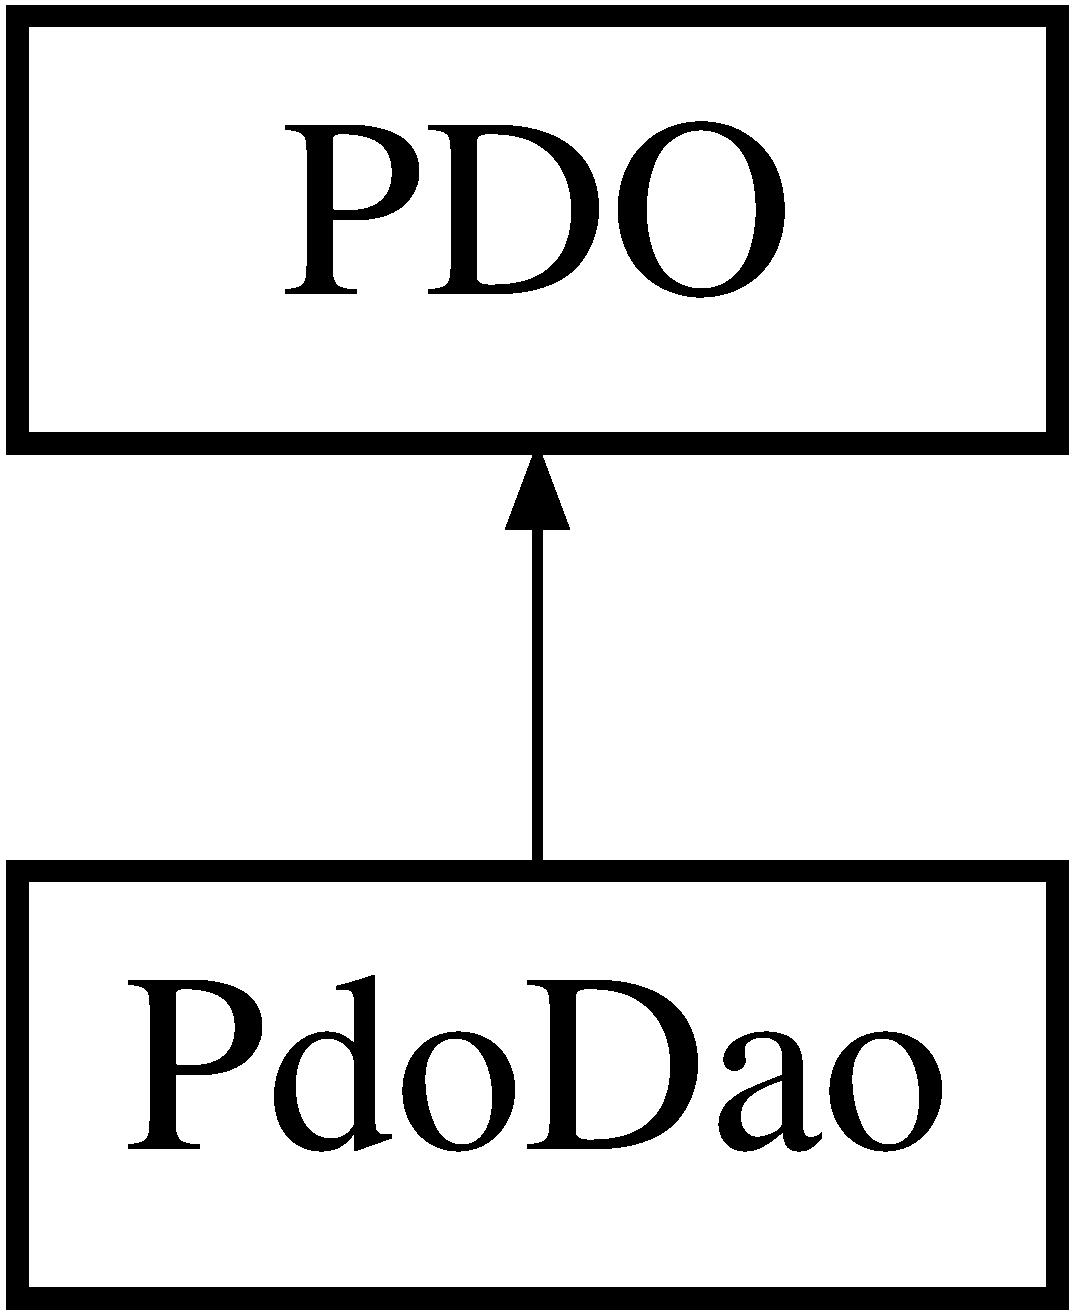
\includegraphics[height=2.000000cm]{class_pdo_dao}
\end{center}
\end{figure}
\subsection*{Public Member Functions}
\begin{DoxyCompactItemize}
\item 
\hyperlink{class_pdo_dao_a095c5d389db211932136b53f25f39685}{\+\_\+\+\_\+construct} ()
\item 
\hyperlink{class_pdo_dao_a12c1ef0decfa06f2f07cb681f3be8c50}{get\+Rows} (\$sql, \$params, \$style)
\item 
\hyperlink{class_pdo_dao_a5ba34a0a513050a7983c8c9f03a30732}{exec\+S\+QL} (\$sql, \$params)
\item 
\hyperlink{class_pdo_dao_a25d71275d800f84b28ec8bd6e055a675}{get\+Value} (\$sql, \$params)
\end{DoxyCompactItemize}


\subsection{Detailed Description}


Definition at line 8 of file Pdo\+Dao.\+class.\+php.



\subsection{Constructor \& Destructor Documentation}
\mbox{\Hypertarget{class_pdo_dao_a095c5d389db211932136b53f25f39685}\label{class_pdo_dao_a095c5d389db211932136b53f25f39685}} 
\index{Pdo\+Dao@{Pdo\+Dao}!\+\_\+\+\_\+construct@{\+\_\+\+\_\+construct}}
\index{\+\_\+\+\_\+construct@{\+\_\+\+\_\+construct}!Pdo\+Dao@{Pdo\+Dao}}
\subsubsection{\texorpdfstring{\+\_\+\+\_\+construct()}{\_\_construct()}}
{\footnotesize\ttfamily \+\_\+\+\_\+construct (\begin{DoxyParamCaption}{ }\end{DoxyParamCaption})}

Constructeur hérité de P\+DO 

Definition at line 13 of file Pdo\+Dao.\+class.\+php.



\subsection{Member Function Documentation}
\mbox{\Hypertarget{class_pdo_dao_a5ba34a0a513050a7983c8c9f03a30732}\label{class_pdo_dao_a5ba34a0a513050a7983c8c9f03a30732}} 
\index{Pdo\+Dao@{Pdo\+Dao}!exec\+S\+QL@{exec\+S\+QL}}
\index{exec\+S\+QL@{exec\+S\+QL}!Pdo\+Dao@{Pdo\+Dao}}
\subsubsection{\texorpdfstring{exec\+S\+Q\+L()}{execSQL()}}
{\footnotesize\ttfamily exec\+S\+QL (\begin{DoxyParamCaption}\item[{}]{\$sql,  }\item[{}]{\$params }\end{DoxyParamCaption})}

Fonction qui exécute une requête action préparée avec des paramètres anonymes 
\begin{DoxyParams}{Parameters}
{\em \$sql} & \+: la requête S\+QL à exécuter \\
\hline
{\em \$params} & \+: un tableau de paramètres contenant les valeurs à substituer dans la requête \\
\hline
\end{DoxyParams}
\begin{DoxyReturn}{Returns}
un entier désignant le nombre de lignes affectées par l\textquotesingle{}exécution de la requête 
\end{DoxyReturn}


Definition at line 66 of file Pdo\+Dao.\+class.\+php.

\mbox{\Hypertarget{class_pdo_dao_a12c1ef0decfa06f2f07cb681f3be8c50}\label{class_pdo_dao_a12c1ef0decfa06f2f07cb681f3be8c50}} 
\index{Pdo\+Dao@{Pdo\+Dao}!get\+Rows@{get\+Rows}}
\index{get\+Rows@{get\+Rows}!Pdo\+Dao@{Pdo\+Dao}}
\subsubsection{\texorpdfstring{get\+Rows()}{getRows()}}
{\footnotesize\ttfamily get\+Rows (\begin{DoxyParamCaption}\item[{}]{\$sql,  }\item[{}]{\$params,  }\item[{}]{\$style }\end{DoxyParamCaption})}

Fonction qui renvoie un tableau de valeurs correspondant au résultat de l\textquotesingle{}exécution d\textquotesingle{}une requête préparée S\+QL avec des paramètres anonymes 
\begin{DoxyParams}{Parameters}
{\em \$sql} & (la requête S\+QL à exécuter) \\
\hline
{\em \$params} & \+: un tableau de paramètres contenant les valeurs \\
\hline
{\em \$style} & \+: 0 == both, 1 == objet \\
\hline
\end{DoxyParams}
\begin{DoxyReturn}{Returns}
un tableau associatif ou \char`\"{}objet\char`\"{} suivant le paramètre style 
\end{DoxyReturn}


Definition at line 39 of file Pdo\+Dao.\+class.\+php.

\mbox{\Hypertarget{class_pdo_dao_a25d71275d800f84b28ec8bd6e055a675}\label{class_pdo_dao_a25d71275d800f84b28ec8bd6e055a675}} 
\index{Pdo\+Dao@{Pdo\+Dao}!get\+Value@{get\+Value}}
\index{get\+Value@{get\+Value}!Pdo\+Dao@{Pdo\+Dao}}
\subsubsection{\texorpdfstring{get\+Value()}{getValue()}}
{\footnotesize\ttfamily get\+Value (\begin{DoxyParamCaption}\item[{}]{\$sql,  }\item[{}]{\$params }\end{DoxyParamCaption})}

Fonction qui exécute une requête préparée avec des paramètres anonymes et qui récupère une seule valeur 
\begin{DoxyParams}{Parameters}
{\em \$sql} & \+: la requête S\+QL à exécuter La requête ne doit renvoyer qu\textquotesingle{}une colonne et une ligne \\
\hline
{\em \$params} & \+: un tableau de paramètres contenant les valeurs à substituer dans la requête \\
\hline
\end{DoxyParams}
\begin{DoxyReturn}{Returns}
la valeur récupérée par l\textquotesingle{}exécution de la requête 
\end{DoxyReturn}


Definition at line 86 of file Pdo\+Dao.\+class.\+php.



The documentation for this class was generated from the following file\+:\begin{DoxyCompactItemize}
\item 
modele/\+Dal/\hyperlink{_pdo_dao_8class_8php}{Pdo\+Dao.\+class.\+php}\end{DoxyCompactItemize}

\hypertarget{class_pret}{}\section{Pret Class Reference}
\label{class_pret}\index{Pret@{Pret}}
\subsection*{Public Member Functions}
\begin{DoxyCompactItemize}
\item 
\hyperlink{class_pret_aff90a1966dd0404d05a530676aec0472}{\+\_\+\+\_\+construct} ( \$p\+\_\+id, \$p\+\_\+client, \$p\+\_\+ouvrage, \$p\+\_\+date\+\_\+emp, \$p\+\_\+date\+\_\+ret, \$p\+\_\+penalite)
\item 
\hyperlink{class_pret_a12251d0c022e9e21c137a105ff683f13}{get\+Id} ()
\item 
\hyperlink{class_pret_a2f5f44fdf5404c87cc3a7b5719d85306}{get\+Client} ()
\item 
\hyperlink{class_pret_a60362b06c32bb1a659f65d6d54857021}{get\+Ouvrage} ()
\item 
\hyperlink{class_pret_afa67d7628b29e3e32469cd070ae19f10}{get\+Date\+Emp} ()
\item 
\hyperlink{class_pret_a85740f396854605d6a989fac86cabba2}{get\+Date\+Ret} ()
\item 
\hyperlink{class_pret_a0eac81d4f3534a285e7abe04dc6a2b4c}{get\+Penalite} ()
\item 
\hyperlink{class_pret_ab2fff0fc655f96b6e5f4fcc294c49eee}{set\+Id} (\$p\+\_\+id)
\item 
\hyperlink{class_pret_addc317db48b6f5bddc99581c2c6464eb}{set\+Client} (\$p\+\_\+client)
\item 
\hyperlink{class_pret_a721ed73a4d5b195a2cf9e0ec9001cad7}{set\+Ouvrage} (\$p\+\_\+ouvrage)
\item 
\hyperlink{class_pret_aa698d4791c453b088a1428cd5244b3bd}{set\+Date\+Emp} (\$p\+\_\+date\+Emp)
\item 
\hyperlink{class_pret_a9235ca829aedf23f31a1d408e9fc9d30}{set\+Date\+Ret} (\$p\+\_\+date\+Ret)
\item 
\hyperlink{class_pret_a91be6085dead298d8a7f2d4358ec8607}{set\+Penalite} (\$p\+\_\+penalite)
\end{DoxyCompactItemize}


\subsection{Detailed Description}


Definition at line 23 of file Pret.\+class.\+php.



\subsection{Constructor \& Destructor Documentation}
\mbox{\Hypertarget{class_pret_aff90a1966dd0404d05a530676aec0472}\label{class_pret_aff90a1966dd0404d05a530676aec0472}} 
\index{Pret@{Pret}!\+\_\+\+\_\+construct@{\+\_\+\+\_\+construct}}
\index{\+\_\+\+\_\+construct@{\+\_\+\+\_\+construct}!Pret@{Pret}}
\subsubsection{\texorpdfstring{\+\_\+\+\_\+construct()}{\_\_construct()}}
{\footnotesize\ttfamily \+\_\+\+\_\+construct (\begin{DoxyParamCaption}\item[{}]{\$p\+\_\+id,  }\item[{}]{\$p\+\_\+client,  }\item[{}]{\$p\+\_\+ouvrage,  }\item[{}]{\$p\+\_\+date\+\_\+emp,  }\item[{}]{\$p\+\_\+date\+\_\+ret,  }\item[{}]{\$p\+\_\+penalite }\end{DoxyParamCaption})}

Constructeur 

Definition at line 34 of file Pret.\+class.\+php.



\subsection{Member Function Documentation}
\mbox{\Hypertarget{class_pret_a2f5f44fdf5404c87cc3a7b5719d85306}\label{class_pret_a2f5f44fdf5404c87cc3a7b5719d85306}} 
\index{Pret@{Pret}!get\+Client@{get\+Client}}
\index{get\+Client@{get\+Client}!Pret@{Pret}}
\subsubsection{\texorpdfstring{get\+Client()}{getClient()}}
{\footnotesize\ttfamily get\+Client (\begin{DoxyParamCaption}{ }\end{DoxyParamCaption})}



Definition at line 57 of file Pret.\+class.\+php.

\mbox{\Hypertarget{class_pret_afa67d7628b29e3e32469cd070ae19f10}\label{class_pret_afa67d7628b29e3e32469cd070ae19f10}} 
\index{Pret@{Pret}!get\+Date\+Emp@{get\+Date\+Emp}}
\index{get\+Date\+Emp@{get\+Date\+Emp}!Pret@{Pret}}
\subsubsection{\texorpdfstring{get\+Date\+Emp()}{getDateEmp()}}
{\footnotesize\ttfamily get\+Date\+Emp (\begin{DoxyParamCaption}{ }\end{DoxyParamCaption})}



Definition at line 65 of file Pret.\+class.\+php.

\mbox{\Hypertarget{class_pret_a85740f396854605d6a989fac86cabba2}\label{class_pret_a85740f396854605d6a989fac86cabba2}} 
\index{Pret@{Pret}!get\+Date\+Ret@{get\+Date\+Ret}}
\index{get\+Date\+Ret@{get\+Date\+Ret}!Pret@{Pret}}
\subsubsection{\texorpdfstring{get\+Date\+Ret()}{getDateRet()}}
{\footnotesize\ttfamily get\+Date\+Ret (\begin{DoxyParamCaption}{ }\end{DoxyParamCaption})}



Definition at line 69 of file Pret.\+class.\+php.

\mbox{\Hypertarget{class_pret_a12251d0c022e9e21c137a105ff683f13}\label{class_pret_a12251d0c022e9e21c137a105ff683f13}} 
\index{Pret@{Pret}!get\+Id@{get\+Id}}
\index{get\+Id@{get\+Id}!Pret@{Pret}}
\subsubsection{\texorpdfstring{get\+Id()}{getId()}}
{\footnotesize\ttfamily get\+Id (\begin{DoxyParamCaption}{ }\end{DoxyParamCaption})}

Accesseurs 

Definition at line 53 of file Pret.\+class.\+php.

\mbox{\Hypertarget{class_pret_a60362b06c32bb1a659f65d6d54857021}\label{class_pret_a60362b06c32bb1a659f65d6d54857021}} 
\index{Pret@{Pret}!get\+Ouvrage@{get\+Ouvrage}}
\index{get\+Ouvrage@{get\+Ouvrage}!Pret@{Pret}}
\subsubsection{\texorpdfstring{get\+Ouvrage()}{getOuvrage()}}
{\footnotesize\ttfamily get\+Ouvrage (\begin{DoxyParamCaption}{ }\end{DoxyParamCaption})}



Definition at line 61 of file Pret.\+class.\+php.

\mbox{\Hypertarget{class_pret_a0eac81d4f3534a285e7abe04dc6a2b4c}\label{class_pret_a0eac81d4f3534a285e7abe04dc6a2b4c}} 
\index{Pret@{Pret}!get\+Penalite@{get\+Penalite}}
\index{get\+Penalite@{get\+Penalite}!Pret@{Pret}}
\subsubsection{\texorpdfstring{get\+Penalite()}{getPenalite()}}
{\footnotesize\ttfamily get\+Penalite (\begin{DoxyParamCaption}{ }\end{DoxyParamCaption})}



Definition at line 73 of file Pret.\+class.\+php.

\mbox{\Hypertarget{class_pret_addc317db48b6f5bddc99581c2c6464eb}\label{class_pret_addc317db48b6f5bddc99581c2c6464eb}} 
\index{Pret@{Pret}!set\+Client@{set\+Client}}
\index{set\+Client@{set\+Client}!Pret@{Pret}}
\subsubsection{\texorpdfstring{set\+Client()}{setClient()}}
{\footnotesize\ttfamily set\+Client (\begin{DoxyParamCaption}\item[{}]{\$p\+\_\+client }\end{DoxyParamCaption})}



Definition at line 85 of file Pret.\+class.\+php.

\mbox{\Hypertarget{class_pret_aa698d4791c453b088a1428cd5244b3bd}\label{class_pret_aa698d4791c453b088a1428cd5244b3bd}} 
\index{Pret@{Pret}!set\+Date\+Emp@{set\+Date\+Emp}}
\index{set\+Date\+Emp@{set\+Date\+Emp}!Pret@{Pret}}
\subsubsection{\texorpdfstring{set\+Date\+Emp()}{setDateEmp()}}
{\footnotesize\ttfamily set\+Date\+Emp (\begin{DoxyParamCaption}\item[{}]{\$p\+\_\+date\+Emp }\end{DoxyParamCaption})}



Definition at line 93 of file Pret.\+class.\+php.

\mbox{\Hypertarget{class_pret_a9235ca829aedf23f31a1d408e9fc9d30}\label{class_pret_a9235ca829aedf23f31a1d408e9fc9d30}} 
\index{Pret@{Pret}!set\+Date\+Ret@{set\+Date\+Ret}}
\index{set\+Date\+Ret@{set\+Date\+Ret}!Pret@{Pret}}
\subsubsection{\texorpdfstring{set\+Date\+Ret()}{setDateRet()}}
{\footnotesize\ttfamily set\+Date\+Ret (\begin{DoxyParamCaption}\item[{}]{\$p\+\_\+date\+Ret }\end{DoxyParamCaption})}



Definition at line 97 of file Pret.\+class.\+php.

\mbox{\Hypertarget{class_pret_ab2fff0fc655f96b6e5f4fcc294c49eee}\label{class_pret_ab2fff0fc655f96b6e5f4fcc294c49eee}} 
\index{Pret@{Pret}!set\+Id@{set\+Id}}
\index{set\+Id@{set\+Id}!Pret@{Pret}}
\subsubsection{\texorpdfstring{set\+Id()}{setId()}}
{\footnotesize\ttfamily set\+Id (\begin{DoxyParamCaption}\item[{}]{\$p\+\_\+id }\end{DoxyParamCaption})}

Mutateurs 

Definition at line 81 of file Pret.\+class.\+php.

\mbox{\Hypertarget{class_pret_a721ed73a4d5b195a2cf9e0ec9001cad7}\label{class_pret_a721ed73a4d5b195a2cf9e0ec9001cad7}} 
\index{Pret@{Pret}!set\+Ouvrage@{set\+Ouvrage}}
\index{set\+Ouvrage@{set\+Ouvrage}!Pret@{Pret}}
\subsubsection{\texorpdfstring{set\+Ouvrage()}{setOuvrage()}}
{\footnotesize\ttfamily set\+Ouvrage (\begin{DoxyParamCaption}\item[{}]{\$p\+\_\+ouvrage }\end{DoxyParamCaption})}



Definition at line 89 of file Pret.\+class.\+php.

\mbox{\Hypertarget{class_pret_a91be6085dead298d8a7f2d4358ec8607}\label{class_pret_a91be6085dead298d8a7f2d4358ec8607}} 
\index{Pret@{Pret}!set\+Penalite@{set\+Penalite}}
\index{set\+Penalite@{set\+Penalite}!Pret@{Pret}}
\subsubsection{\texorpdfstring{set\+Penalite()}{setPenalite()}}
{\footnotesize\ttfamily set\+Penalite (\begin{DoxyParamCaption}\item[{}]{\$p\+\_\+penalite }\end{DoxyParamCaption})}



Definition at line 101 of file Pret.\+class.\+php.



The documentation for this class was generated from the following file\+:\begin{DoxyCompactItemize}
\item 
modele/\+Reference/\hyperlink{_pret_8class_8php}{Pret.\+class.\+php}\end{DoxyCompactItemize}

\hypertarget{class_pret_dal}{}\section{Pret\+Dal Class Reference}
\label{class_pret_dal}\index{Pret\+Dal@{Pret\+Dal}}
\subsection*{Static Public Member Functions}
\begin{DoxyCompactItemize}
\item 
static \hyperlink{class_pret_dal_a64160420395c456d3b8156ea4c50debf}{load\+Generic\+Pret} (\$mode, \$array\+Params)
\item 
static \hyperlink{class_pret_dal_ade787cbf441d30de9f3838f7e8d6cb37}{add\+Pret} (\$no\+\_\+client, \$no\+\_\+ouvrage, \$date\+\_\+emp)
\end{DoxyCompactItemize}


\subsection{Detailed Description}


Definition at line 19 of file Pret\+Dal.\+class.\+php.



\subsection{Member Function Documentation}
\mbox{\Hypertarget{class_pret_dal_ade787cbf441d30de9f3838f7e8d6cb37}\label{class_pret_dal_ade787cbf441d30de9f3838f7e8d6cb37}} 
\index{Pret\+Dal@{Pret\+Dal}!add\+Pret@{add\+Pret}}
\index{add\+Pret@{add\+Pret}!Pret\+Dal@{Pret\+Dal}}
\subsubsection{\texorpdfstring{add\+Pret()}{addPret()}}
{\footnotesize\ttfamily static add\+Pret (\begin{DoxyParamCaption}\item[{}]{\$no\+\_\+client,  }\item[{}]{\$no\+\_\+ouvrage,  }\item[{}]{\$date\+\_\+emp }\end{DoxyParamCaption})\hspace{0.3cm}{\ttfamily [static]}}

\begin{DoxyAuthor}{Author}
PV G2 11/11/2016 
\end{DoxyAuthor}

\begin{DoxyParams}[1]{Parameters}
int & {\em \$no\+\_\+client} & le numéro du cient emprunteur \\
\hline
int & {\em \$no\+\_\+ouvrage} & le numéro de l\textquotesingle{}ouvrage emprunté \\
\hline
date & {\em \$date\+\_\+emp} & la date d\textquotesingle{}emprunt de l\textquotesingle{}ouvrage \\
\hline
\end{DoxyParams}
\begin{DoxyReturn}{Returns}
\hyperlink{class_pret}{Pret} un objet de la classe \hyperlink{class_pret}{Pret} 
\end{DoxyReturn}


Definition at line 78 of file Pret\+Dal.\+class.\+php.

\mbox{\Hypertarget{class_pret_dal_a64160420395c456d3b8156ea4c50debf}\label{class_pret_dal_a64160420395c456d3b8156ea4c50debf}} 
\index{Pret\+Dal@{Pret\+Dal}!load\+Generic\+Pret@{load\+Generic\+Pret}}
\index{load\+Generic\+Pret@{load\+Generic\+Pret}!Pret\+Dal@{Pret\+Dal}}
\subsubsection{\texorpdfstring{load\+Generic\+Pret()}{loadGenericPret()}}
{\footnotesize\ttfamily static load\+Generic\+Pret (\begin{DoxyParamCaption}\item[{}]{\$mode,  }\item[{}]{\$array\+Params }\end{DoxyParamCaption})\hspace{0.3cm}{\ttfamily [static]}}

\begin{DoxyAuthor}{Author}
PV G2 10/11/2016 load\+Generic\+Pret est une fonction générique permettant de charger des prêts 
\end{DoxyAuthor}

\begin{DoxyParams}[1]{Parameters}
int & {\em \$mode} & 0 =$>$ charge tous les prêts de tous les clients avec etat optionel, 1 =$>$ charge un prêts par id, 2 =$>$ charge tous les prêts d\textquotesingle{}un clients par etat \\
\hline
array & {\em \$array\+Params} & si mode 0 donné un état de prêts (voir config.\+inc.\+php), si mode 1 mettre un id de pret dans le tableau, si mode 2 mettre un numéro de client et un état de prêts (voir config.\+inc.\+php) \\
\hline
\end{DoxyParams}
\begin{DoxyReturn}{Returns}
mixed =$>$ si les paramétres de la fonction ne concorde pas avec le mode utilisé, la fonctions retournera false =$>$ si l\textquotesingle{}exécution se déroule normalement la fonction retourne le résultat de l\textquotesingle{}appel à la procédure stockée$<$ 
\end{DoxyReturn}


Definition at line 32 of file Pret\+Dal.\+class.\+php.



The documentation for this class was generated from the following file\+:\begin{DoxyCompactItemize}
\item 
modele/\+Dal/\hyperlink{_pret_dal_8class_8php}{Pret\+Dal.\+class.\+php}\end{DoxyCompactItemize}

\hypertarget{class_prets}{}\section{Prets Class Reference}
\label{class_prets}\index{Prets@{Prets}}
\subsection*{Static Public Member Functions}
\begin{DoxyCompactItemize}
\item 
static \hyperlink{class_prets_a8a173fad71ea1b75ea7fb092732bd7fb}{charger\+Les\+Prets} (\$mode, \$etat\+\_\+pret)
\item 
static \hyperlink{class_prets_ae2e15f8376a62a7e410b70431a365e4f}{pret\+Existe} (\$id)
\item 
static \hyperlink{class_prets_af21bb9078a59c621c5539fd14716e689}{ajouter\+Pret} (\$no\+\_\+client, \$no\+\_\+ouvrage, \$date\+\_\+emp)
\item 
static \hyperlink{class_prets_a71f7b77d9ff38020ab022389dda0e226}{modifier\+Pret} (\$pret)
\item 
static \hyperlink{class_prets_a319222a4f2442b93068fadd2a5bb7d2d}{supprimer\+Pret} (\$id)
\item 
static \hyperlink{class_prets_a7ea0e0fc80de1d6df26d9a8e0017ff92}{charger\+Pret\+Par\+Id} (\$id)
\end{DoxyCompactItemize}


\subsection{Detailed Description}


Definition at line 35 of file Prets.\+class.\+php.



\subsection{Member Function Documentation}
\mbox{\Hypertarget{class_prets_af21bb9078a59c621c5539fd14716e689}\label{class_prets_af21bb9078a59c621c5539fd14716e689}} 
\index{Prets@{Prets}!ajouter\+Pret@{ajouter\+Pret}}
\index{ajouter\+Pret@{ajouter\+Pret}!Prets@{Prets}}
\subsubsection{\texorpdfstring{ajouter\+Pret()}{ajouterPret()}}
{\footnotesize\ttfamily static ajouter\+Pret (\begin{DoxyParamCaption}\item[{}]{\$no\+\_\+client,  }\item[{}]{\$no\+\_\+ouvrage,  }\item[{}]{\$date\+\_\+emp }\end{DoxyParamCaption})\hspace{0.3cm}{\ttfamily [static]}}

\begin{DoxyAuthor}{Author}
PV 18/11/2016 
\end{DoxyAuthor}

\begin{DoxyParams}[1]{Parameters}
int & {\em \$no\+\_\+client} & le numéro du cient emprunteur \\
\hline
int & {\em \$no\+\_\+ouvrage} & le numéro de l\textquotesingle{}ouvrage emprunté \\
\hline
date & {\em \$date\+\_\+emp} & la date d\textquotesingle{}emprunt de l\textquotesingle{}ouvrage \\
\hline
\end{DoxyParams}
\begin{DoxyReturn}{Returns}
int \$result 0 =$>$ l\textquotesingle{}ajout à été normalement effectué -\/1 =$>$ aucun numéro de client n\textquotesingle{}à été transmis à la procédure -\/2 =$>$ le client n\textquotesingle{}existe pas -\/4 =$>$ aucun numéro d\textquotesingle{}ouvrage n\textquotesingle{}à été transmis à la procédure -\/6 =$>$ l\textquotesingle{}ouvrage n\textquotesingle{}existe pas -\/8 =$>$ aucune date d\textquotesingle{}emprunt transmise à la procédure -\/10 =$>$ l\textquotesingle{}ouvrage que l\textquotesingle{}on souhaite emprunté est déjà prêté -\/99 =$>$ La requête à échoué 
\end{DoxyReturn}


Definition at line 94 of file Prets.\+class.\+php.

\mbox{\Hypertarget{class_prets_a8a173fad71ea1b75ea7fb092732bd7fb}\label{class_prets_a8a173fad71ea1b75ea7fb092732bd7fb}} 
\index{Prets@{Prets}!charger\+Les\+Prets@{charger\+Les\+Prets}}
\index{charger\+Les\+Prets@{charger\+Les\+Prets}!Prets@{Prets}}
\subsubsection{\texorpdfstring{charger\+Les\+Prets()}{chargerLesPrets()}}
{\footnotesize\ttfamily static charger\+Les\+Prets (\begin{DoxyParamCaption}\item[{}]{\$mode,  }\item[{}]{\$etat\+\_\+pret }\end{DoxyParamCaption})\hspace{0.3cm}{\ttfamily [static]}}

Méthodes publiques \begin{DoxyAuthor}{Author}
PV G2 10/11/2016 récupére les prets 
\end{DoxyAuthor}

\begin{DoxyParams}{Parameters}
{\em \$mode} & \+: 0 == tableau assoc, 1 == tableau d\textquotesingle{}objets \$etat\+\_\+pret \+: voir config.\+inc.\+php rubrique \char`\"{}constantes pour la fonction load\+Generic\+Pret\char`\"{} \\
\hline
\end{DoxyParams}
\begin{DoxyReturn}{Returns}
un tableau de type \$mode 
\end{DoxyReturn}


Definition at line 47 of file Prets.\+class.\+php.

\mbox{\Hypertarget{class_prets_a7ea0e0fc80de1d6df26d9a8e0017ff92}\label{class_prets_a7ea0e0fc80de1d6df26d9a8e0017ff92}} 
\index{Prets@{Prets}!charger\+Pret\+Par\+Id@{charger\+Pret\+Par\+Id}}
\index{charger\+Pret\+Par\+Id@{charger\+Pret\+Par\+Id}!Prets@{Prets}}
\subsubsection{\texorpdfstring{charger\+Pret\+Par\+Id()}{chargerPretParId()}}
{\footnotesize\ttfamily static charger\+Pret\+Par\+Id (\begin{DoxyParamCaption}\item[{}]{\$id }\end{DoxyParamCaption})\hspace{0.3cm}{\ttfamily [static]}}

\begin{DoxyAuthor}{Author}
G2 17/11/2016 récupére les caractéristiques d\textquotesingle{}un pret 
\end{DoxyAuthor}

\begin{DoxyParams}{Parameters}
{\em \$id} & \+: le code du pret \\
\hline
\end{DoxyParams}
\begin{DoxyReturn}{Returns}
un objet de la classe pret 
\end{DoxyReturn}


Definition at line 120 of file Prets.\+class.\+php.

\mbox{\Hypertarget{class_prets_a71f7b77d9ff38020ab022389dda0e226}\label{class_prets_a71f7b77d9ff38020ab022389dda0e226}} 
\index{Prets@{Prets}!modifier\+Pret@{modifier\+Pret}}
\index{modifier\+Pret@{modifier\+Pret}!Prets@{Prets}}
\subsubsection{\texorpdfstring{modifier\+Pret()}{modifierPret()}}
{\footnotesize\ttfamily static modifier\+Pret (\begin{DoxyParamCaption}\item[{}]{\$pret }\end{DoxyParamCaption})\hspace{0.3cm}{\ttfamily [static]}}



Definition at line 104 of file Prets.\+class.\+php.

\mbox{\Hypertarget{class_prets_ae2e15f8376a62a7e410b70431a365e4f}\label{class_prets_ae2e15f8376a62a7e410b70431a365e4f}} 
\index{Prets@{Prets}!pret\+Existe@{pret\+Existe}}
\index{pret\+Existe@{pret\+Existe}!Prets@{Prets}}
\subsubsection{\texorpdfstring{pret\+Existe()}{pretExiste()}}
{\footnotesize\ttfamily static pret\+Existe (\begin{DoxyParamCaption}\item[{}]{\$id }\end{DoxyParamCaption})\hspace{0.3cm}{\ttfamily [static]}}

\begin{DoxyAuthor}{Author}
dk vérifie si un pret existe 
\end{DoxyAuthor}

\begin{DoxyParams}{Parameters}
{\em \$id} & \+: le code du pret é contréler \\
\hline
\end{DoxyParams}
\begin{DoxyReturn}{Returns}
un booléen 
\end{DoxyReturn}


Definition at line 72 of file Prets.\+class.\+php.

\mbox{\Hypertarget{class_prets_a319222a4f2442b93068fadd2a5bb7d2d}\label{class_prets_a319222a4f2442b93068fadd2a5bb7d2d}} 
\index{Prets@{Prets}!supprimer\+Pret@{supprimer\+Pret}}
\index{supprimer\+Pret@{supprimer\+Pret}!Prets@{Prets}}
\subsubsection{\texorpdfstring{supprimer\+Pret()}{supprimerPret()}}
{\footnotesize\ttfamily static supprimer\+Pret (\begin{DoxyParamCaption}\item[{}]{\$id }\end{DoxyParamCaption})\hspace{0.3cm}{\ttfamily [static]}}



Definition at line 110 of file Prets.\+class.\+php.



The documentation for this class was generated from the following file\+:\begin{DoxyCompactItemize}
\item 
modele/\+Bll/\hyperlink{_prets_8class_8php}{Prets.\+class.\+php}\end{DoxyCompactItemize}

\hypertarget{class_utilities}{}\section{Utilities Class Reference}
\label{class_utilities}\index{Utilities@{Utilities}}
\subsection*{Static Public Member Functions}
\begin{DoxyCompactItemize}
\item 
static \hyperlink{class_utilities_af36aa51d20191f7718d33418001af3fb}{is\+Pos\+Int} (\$valeur)
\item 
static \hyperlink{class_utilities_a932a96b8eac601a1842e040c703657a5}{get\+Day} (\$date)
\item 
static \hyperlink{class_utilities_a7d6905a273f76e42d3ae5021248d2ed0}{get\+Year} (\$date)
\item 
static \hyperlink{class_utilities_ae2079f81b1e43b78deddc4bb77cb6c68}{get\+Month} (\$date, \$mode)
\item 
static \hyperlink{class_utilities_aed4a7fe88d85a1b64ebca49b5b8c8aa9}{get\+Str\+Day} (\$day)
\item 
static \hyperlink{class_utilities_a47fb2f7c80a9da546689e7ff188aa58b}{get\+Int\+Day} (\$day)
\item 
static \hyperlink{class_utilities_ab9b0bb93c5d3f205617398e33c1d1ea4}{get\+Jour\+Francais} (\$day)
\item 
static \hyperlink{class_utilities_aae99ab6f0743ff6fec92fb580916051e}{get\+Date\+Francais} (\$date)
\item 
static \hyperlink{class_utilities_a32a363b47bdf72b917ffd354dfcd2cb6}{get\+Date\+Francais\+Mois\+Annee} (\$date)
\item 
static \hyperlink{class_utilities_a9c7006be389743193fe09b92b5d57e3f}{get\+Dernier\+Jour\+Mois} (\$annee, \$mois)
\item 
static \hyperlink{class_utilities_ac554970f7f045a6373fc80aacfd3c11b}{annee\+Est\+Bissextile} (\$annee)
\item 
static \hyperlink{class_utilities_a34945d34c0465e88799eaeda066dfb53}{nb\+Files} (\$dir)
\item 
static \hyperlink{class_utilities_a3db97c6e1efe4c47efaf00d4e5f2163a}{first\+Occur} (\$tab, \$mode=0)
\item 
static \hyperlink{class_utilities_a4151d2b42a0b24dd9fdf6bc3823e6bda}{is\+Date} (\$date)
\item 
static \hyperlink{class_utilities_afdefc03981b517dfe3bf6c9f788b4c8d}{operation\+Date} (\$date\+One, \$datetwo, \$operateur)
\end{DoxyCompactItemize}


\subsection{Detailed Description}


Definition at line 13 of file Utilities.\+class.\+php.



\subsection{Member Function Documentation}
\mbox{\Hypertarget{class_utilities_ac554970f7f045a6373fc80aacfd3c11b}\label{class_utilities_ac554970f7f045a6373fc80aacfd3c11b}} 
\index{Utilities@{Utilities}!annee\+Est\+Bissextile@{annee\+Est\+Bissextile}}
\index{annee\+Est\+Bissextile@{annee\+Est\+Bissextile}!Utilities@{Utilities}}
\subsubsection{\texorpdfstring{annee\+Est\+Bissextile()}{anneeEstBissextile()}}
{\footnotesize\ttfamily static annee\+Est\+Bissextile (\begin{DoxyParamCaption}\item[{}]{\$annee }\end{DoxyParamCaption})\hspace{0.3cm}{\ttfamily [static]}}



Definition at line 343 of file Utilities.\+class.\+php.

\mbox{\Hypertarget{class_utilities_a3db97c6e1efe4c47efaf00d4e5f2163a}\label{class_utilities_a3db97c6e1efe4c47efaf00d4e5f2163a}} 
\index{Utilities@{Utilities}!first\+Occur@{first\+Occur}}
\index{first\+Occur@{first\+Occur}!Utilities@{Utilities}}
\subsubsection{\texorpdfstring{first\+Occur()}{firstOccur()}}
{\footnotesize\ttfamily static first\+Occur (\begin{DoxyParamCaption}\item[{}]{\$tab,  }\item[{}]{\$mode = {\ttfamily 0} }\end{DoxyParamCaption})\hspace{0.3cm}{\ttfamily [static]}}

\begin{DoxyAuthor}{Author}
PV G2 21/11/2016 Retourne la premiére clé/valeur d\textquotesingle{}un tableau (notament utile pour les tableaux associatifs) 
\end{DoxyAuthor}

\begin{DoxyParams}[1]{Parameters}
array & {\em \$tab} & un tableau \\
\hline
int & {\em \$mode} & 0 =$>$ renvoie la premiére valeur du tableau, 1=$>$ renvoie la premiére clé du tableau \\
\hline
\end{DoxyParams}
\begin{DoxyReturn}{Returns}
mixed la premiére occurence d\textquotesingle{}un tableau ou nul si le tableau est vide 
\end{DoxyReturn}


Definition at line 379 of file Utilities.\+class.\+php.

\mbox{\Hypertarget{class_utilities_aae99ab6f0743ff6fec92fb580916051e}\label{class_utilities_aae99ab6f0743ff6fec92fb580916051e}} 
\index{Utilities@{Utilities}!get\+Date\+Francais@{get\+Date\+Francais}}
\index{get\+Date\+Francais@{get\+Date\+Francais}!Utilities@{Utilities}}
\subsubsection{\texorpdfstring{get\+Date\+Francais()}{getDateFrancais()}}
{\footnotesize\ttfamily static get\+Date\+Francais (\begin{DoxyParamCaption}\item[{}]{\$date }\end{DoxyParamCaption})\hspace{0.3cm}{\ttfamily [static]}}



Definition at line 298 of file Utilities.\+class.\+php.

\mbox{\Hypertarget{class_utilities_a32a363b47bdf72b917ffd354dfcd2cb6}\label{class_utilities_a32a363b47bdf72b917ffd354dfcd2cb6}} 
\index{Utilities@{Utilities}!get\+Date\+Francais\+Mois\+Annee@{get\+Date\+Francais\+Mois\+Annee}}
\index{get\+Date\+Francais\+Mois\+Annee@{get\+Date\+Francais\+Mois\+Annee}!Utilities@{Utilities}}
\subsubsection{\texorpdfstring{get\+Date\+Francais\+Mois\+Annee()}{getDateFrancaisMoisAnnee()}}
{\footnotesize\ttfamily static get\+Date\+Francais\+Mois\+Annee (\begin{DoxyParamCaption}\item[{}]{\$date }\end{DoxyParamCaption})\hspace{0.3cm}{\ttfamily [static]}}



Definition at line 302 of file Utilities.\+class.\+php.

\mbox{\Hypertarget{class_utilities_a932a96b8eac601a1842e040c703657a5}\label{class_utilities_a932a96b8eac601a1842e040c703657a5}} 
\index{Utilities@{Utilities}!get\+Day@{get\+Day}}
\index{get\+Day@{get\+Day}!Utilities@{Utilities}}
\subsubsection{\texorpdfstring{get\+Day()}{getDay()}}
{\footnotesize\ttfamily static get\+Day (\begin{DoxyParamCaption}\item[{}]{\$date }\end{DoxyParamCaption})\hspace{0.3cm}{\ttfamily [static]}}

Retourne le jour d\textquotesingle{}une date 
\begin{DoxyParams}{Parameters}
{\em \$date} & \+: un objet  \\
\hline
\end{DoxyParams}
\begin{DoxyReturn}{Returns}
le jour 
\end{DoxyReturn}


Definition at line 33 of file Utilities.\+class.\+php.

\mbox{\Hypertarget{class_utilities_a9c7006be389743193fe09b92b5d57e3f}\label{class_utilities_a9c7006be389743193fe09b92b5d57e3f}} 
\index{Utilities@{Utilities}!get\+Dernier\+Jour\+Mois@{get\+Dernier\+Jour\+Mois}}
\index{get\+Dernier\+Jour\+Mois@{get\+Dernier\+Jour\+Mois}!Utilities@{Utilities}}
\subsubsection{\texorpdfstring{get\+Dernier\+Jour\+Mois()}{getDernierJourMois()}}
{\footnotesize\ttfamily static get\+Dernier\+Jour\+Mois (\begin{DoxyParamCaption}\item[{}]{\$annee,  }\item[{}]{\$mois }\end{DoxyParamCaption})\hspace{0.3cm}{\ttfamily [static]}}



Definition at line 306 of file Utilities.\+class.\+php.

\mbox{\Hypertarget{class_utilities_a47fb2f7c80a9da546689e7ff188aa58b}\label{class_utilities_a47fb2f7c80a9da546689e7ff188aa58b}} 
\index{Utilities@{Utilities}!get\+Int\+Day@{get\+Int\+Day}}
\index{get\+Int\+Day@{get\+Int\+Day}!Utilities@{Utilities}}
\subsubsection{\texorpdfstring{get\+Int\+Day()}{getIntDay()}}
{\footnotesize\ttfamily static get\+Int\+Day (\begin{DoxyParamCaption}\item[{}]{\$day }\end{DoxyParamCaption})\hspace{0.3cm}{\ttfamily [static]}}



Definition at line 214 of file Utilities.\+class.\+php.

\mbox{\Hypertarget{class_utilities_ab9b0bb93c5d3f205617398e33c1d1ea4}\label{class_utilities_ab9b0bb93c5d3f205617398e33c1d1ea4}} 
\index{Utilities@{Utilities}!get\+Jour\+Francais@{get\+Jour\+Francais}}
\index{get\+Jour\+Francais@{get\+Jour\+Francais}!Utilities@{Utilities}}
\subsubsection{\texorpdfstring{get\+Jour\+Francais()}{getJourFrancais()}}
{\footnotesize\ttfamily static get\+Jour\+Francais (\begin{DoxyParamCaption}\item[{}]{\$day }\end{DoxyParamCaption})\hspace{0.3cm}{\ttfamily [static]}}



Definition at line 261 of file Utilities.\+class.\+php.

\mbox{\Hypertarget{class_utilities_ae2079f81b1e43b78deddc4bb77cb6c68}\label{class_utilities_ae2079f81b1e43b78deddc4bb77cb6c68}} 
\index{Utilities@{Utilities}!get\+Month@{get\+Month}}
\index{get\+Month@{get\+Month}!Utilities@{Utilities}}
\subsubsection{\texorpdfstring{get\+Month()}{getMonth()}}
{\footnotesize\ttfamily static get\+Month (\begin{DoxyParamCaption}\item[{}]{\$date,  }\item[{}]{\$mode }\end{DoxyParamCaption})\hspace{0.3cm}{\ttfamily [static]}}

Retourne le mois d\textquotesingle{}une date exprimé en français \begin{DoxyDate}{Date}
\+: une chaîne représentant une date ou un numéro de mois  \+: 1 == le mois en entier, 2 == le mois abrégé 
\end{DoxyDate}
\begin{DoxyReturn}{Returns}
le mois 
\end{DoxyReturn}


Definition at line 62 of file Utilities.\+class.\+php.

\mbox{\Hypertarget{class_utilities_aed4a7fe88d85a1b64ebca49b5b8c8aa9}\label{class_utilities_aed4a7fe88d85a1b64ebca49b5b8c8aa9}} 
\index{Utilities@{Utilities}!get\+Str\+Day@{get\+Str\+Day}}
\index{get\+Str\+Day@{get\+Str\+Day}!Utilities@{Utilities}}
\subsubsection{\texorpdfstring{get\+Str\+Day()}{getStrDay()}}
{\footnotesize\ttfamily static get\+Str\+Day (\begin{DoxyParamCaption}\item[{}]{\$day }\end{DoxyParamCaption})\hspace{0.3cm}{\ttfamily [static]}}



Definition at line 177 of file Utilities.\+class.\+php.

\mbox{\Hypertarget{class_utilities_a7d6905a273f76e42d3ae5021248d2ed0}\label{class_utilities_a7d6905a273f76e42d3ae5021248d2ed0}} 
\index{Utilities@{Utilities}!get\+Year@{get\+Year}}
\index{get\+Year@{get\+Year}!Utilities@{Utilities}}
\subsubsection{\texorpdfstring{get\+Year()}{getYear()}}
{\footnotesize\ttfamily static get\+Year (\begin{DoxyParamCaption}\item[{}]{\$date }\end{DoxyParamCaption})\hspace{0.3cm}{\ttfamily [static]}}

Retourne l\textquotesingle{}année d\textquotesingle{}une date \$date \+: un objet  \begin{DoxyReturn}{Returns}
l\textquotesingle{}année 
\end{DoxyReturn}


Definition at line 47 of file Utilities.\+class.\+php.

\mbox{\Hypertarget{class_utilities_a4151d2b42a0b24dd9fdf6bc3823e6bda}\label{class_utilities_a4151d2b42a0b24dd9fdf6bc3823e6bda}} 
\index{Utilities@{Utilities}!is\+Date@{is\+Date}}
\index{is\+Date@{is\+Date}!Utilities@{Utilities}}
\subsubsection{\texorpdfstring{is\+Date()}{isDate()}}
{\footnotesize\ttfamily static is\+Date (\begin{DoxyParamCaption}\item[{}]{\$date }\end{DoxyParamCaption})\hspace{0.3cm}{\ttfamily [static]}}

\begin{DoxyAuthor}{Author}
PV G2 21/11/2016 Indique si une valeur est une date au format dd/mm/\+Y\+Y\+YY (format standard européen) 
\end{DoxyAuthor}

\begin{DoxyParams}{Parameters}
{\em \$date} & une valeur à tester \\
\hline
\end{DoxyParams}
\begin{DoxyReturn}{Returns}
boolean vrai ou faux 
\end{DoxyReturn}


Definition at line 399 of file Utilities.\+class.\+php.

\mbox{\Hypertarget{class_utilities_af36aa51d20191f7718d33418001af3fb}\label{class_utilities_af36aa51d20191f7718d33418001af3fb}} 
\index{Utilities@{Utilities}!is\+Pos\+Int@{is\+Pos\+Int}}
\index{is\+Pos\+Int@{is\+Pos\+Int}!Utilities@{Utilities}}
\subsubsection{\texorpdfstring{is\+Pos\+Int()}{isPosInt()}}
{\footnotesize\ttfamily static is\+Pos\+Int (\begin{DoxyParamCaption}\item[{}]{\$valeur }\end{DoxyParamCaption})\hspace{0.3cm}{\ttfamily [static]}}

Indique si une valeur est un entier positif ou nul 
\begin{DoxyParams}{Parameters}
{\em \$valeur} & \+: la valeur à tester \\
\hline
\end{DoxyParams}
\begin{DoxyReturn}{Returns}
vrai ou faux 
\end{DoxyReturn}


Definition at line 20 of file Utilities.\+class.\+php.

\mbox{\Hypertarget{class_utilities_a34945d34c0465e88799eaeda066dfb53}\label{class_utilities_a34945d34c0465e88799eaeda066dfb53}} 
\index{Utilities@{Utilities}!nb\+Files@{nb\+Files}}
\index{nb\+Files@{nb\+Files}!Utilities@{Utilities}}
\subsubsection{\texorpdfstring{nb\+Files()}{nbFiles()}}
{\footnotesize\ttfamily static nb\+Files (\begin{DoxyParamCaption}\item[{}]{\$dir }\end{DoxyParamCaption})\hspace{0.3cm}{\ttfamily [static]}}

Retourne le nombre de fichiers dans un dossier 
\begin{DoxyParams}[1]{Parameters}
string & {\em \$dir} & \+: le nom du dossier \\
\hline
\end{DoxyParams}
\begin{DoxyReturn}{Returns}
le nombre de fichiers 
\end{DoxyReturn}


Definition at line 360 of file Utilities.\+class.\+php.

\mbox{\Hypertarget{class_utilities_afdefc03981b517dfe3bf6c9f788b4c8d}\label{class_utilities_afdefc03981b517dfe3bf6c9f788b4c8d}} 
\index{Utilities@{Utilities}!operation\+Date@{operation\+Date}}
\index{operation\+Date@{operation\+Date}!Utilities@{Utilities}}
\subsubsection{\texorpdfstring{operation\+Date()}{operationDate()}}
{\footnotesize\ttfamily static operation\+Date (\begin{DoxyParamCaption}\item[{}]{\$date\+One,  }\item[{}]{\$datetwo,  }\item[{}]{\$operateur }\end{DoxyParamCaption})\hspace{0.3cm}{\ttfamily [static]}}

\begin{DoxyAuthor}{Author}
PV G2 21/11/2016 operation\+Date \+: retourne en nombre de jour le résultat d\textquotesingle{}une opération entre deux dates  string \+: \$date\+One La plus ancienne date (au format standard php (Y\+Y\+Y\+Y-\/\+M\+M-\/\+DD))  string \+: \$date\+One La date la plus récente (au format standard php (Y\+Y\+Y\+Y-\/\+M\+M-\/\+DD))  \+: \$operateur l\textquotesingle{}opérateur (le signe) de l\textquotesingle{}opération à effectuer 
\end{DoxyAuthor}
\begin{DoxyReturn}{Returns}
\+: un nombre de jour sous forme d\textquotesingle{}entier 
\end{DoxyReturn}


Definition at line 445 of file Utilities.\+class.\+php.



The documentation for this class was generated from the following file\+:\begin{DoxyCompactItemize}
\item 
modele/\+App/\hyperlink{_utilities_8class_8php}{Utilities.\+class.\+php}\end{DoxyCompactItemize}

\chapter{File Documentation}
\hypertarget{c__gerer_auteurs_8php}{}\section{controleurs/c\+\_\+gerer\+Auteurs.php File Reference}
\label{c__gerer_auteurs_8php}\index{controleurs/c\+\_\+gerer\+Auteurs.\+php@{controleurs/c\+\_\+gerer\+Auteurs.\+php}}
\subsection*{Namespaces}
\begin{DoxyCompactItemize}
\item 
 \hyperlink{namespacedefault}{default}
\end{DoxyCompactItemize}
\subsection*{Variables}
\begin{DoxyCompactItemize}
\item 
if(isset(\$\+\_\+\+G\+ET\mbox{[}\char`\"{}action\char`\"{}\mbox{]})) \hyperlink{c__gerer_auteurs_8php_aa4db7f7a27517cf5cd3ff1f2577caa64}{else}
\item 
if(isset(\$\+\_\+\+R\+E\+Q\+U\+E\+ST\mbox{[}\char`\"{}id\char`\"{}\mbox{]})) \hyperlink{c__gerer_auteurs_8php_a9c2ce5d31a149b2ea7e5ed02e909eb9d}{\$titre\+Page} = \textquotesingle{}Gestion des auteurs\textquotesingle{}
\item 
\hyperlink{c__gerer_auteurs_8php_aaab0cf947dbef94de72bc55c49555684}{\$tab\+Erreurs} = array()
\item 
\hyperlink{c__gerer_auteurs_8php_a81a09ee6e45696499031397e176df7ca}{\$has\+Errors} = false
\item 
\hyperlink{c__gerer_auteurs_8php_a1cab333b177ae7c120b4c2674b30ce86}{\$cnx} = new \hyperlink{class_pdo_dao}{Pdo\+Dao}()
\end{DoxyCompactItemize}


\subsection{Variable Documentation}
\mbox{\Hypertarget{c__gerer_auteurs_8php_a1cab333b177ae7c120b4c2674b30ce86}\label{c__gerer_auteurs_8php_a1cab333b177ae7c120b4c2674b30ce86}} 
\index{c\+\_\+gerer\+Auteurs.\+php@{c\+\_\+gerer\+Auteurs.\+php}!\$cnx@{\$cnx}}
\index{\$cnx@{\$cnx}!c\+\_\+gerer\+Auteurs.\+php@{c\+\_\+gerer\+Auteurs.\+php}}
\subsubsection{\texorpdfstring{\$cnx}{$cnx}}
{\footnotesize\ttfamily \$cnx = new \hyperlink{class_pdo_dao}{Pdo\+Dao}()}



Definition at line 37 of file c\+\_\+gerer\+Auteurs.\+php.

\mbox{\Hypertarget{c__gerer_auteurs_8php_a81a09ee6e45696499031397e176df7ca}\label{c__gerer_auteurs_8php_a81a09ee6e45696499031397e176df7ca}} 
\index{c\+\_\+gerer\+Auteurs.\+php@{c\+\_\+gerer\+Auteurs.\+php}!\$has\+Errors@{\$has\+Errors}}
\index{\$has\+Errors@{\$has\+Errors}!c\+\_\+gerer\+Auteurs.\+php@{c\+\_\+gerer\+Auteurs.\+php}}
\subsubsection{\texorpdfstring{\$has\+Errors}{$hasErrors}}
{\footnotesize\ttfamily \$has\+Errors = false}



Definition at line 34 of file c\+\_\+gerer\+Auteurs.\+php.

\mbox{\Hypertarget{c__gerer_auteurs_8php_aaab0cf947dbef94de72bc55c49555684}\label{c__gerer_auteurs_8php_aaab0cf947dbef94de72bc55c49555684}} 
\index{c\+\_\+gerer\+Auteurs.\+php@{c\+\_\+gerer\+Auteurs.\+php}!\$tab\+Erreurs@{\$tab\+Erreurs}}
\index{\$tab\+Erreurs@{\$tab\+Erreurs}!c\+\_\+gerer\+Auteurs.\+php@{c\+\_\+gerer\+Auteurs.\+php}}
\subsubsection{\texorpdfstring{\$tab\+Erreurs}{$tabErreurs}}
{\footnotesize\ttfamily \$tab\+Erreurs = array()}



Definition at line 33 of file c\+\_\+gerer\+Auteurs.\+php.

\mbox{\Hypertarget{c__gerer_auteurs_8php_a9c2ce5d31a149b2ea7e5ed02e909eb9d}\label{c__gerer_auteurs_8php_a9c2ce5d31a149b2ea7e5ed02e909eb9d}} 
\index{c\+\_\+gerer\+Auteurs.\+php@{c\+\_\+gerer\+Auteurs.\+php}!\$titre\+Page@{\$titre\+Page}}
\index{\$titre\+Page@{\$titre\+Page}!c\+\_\+gerer\+Auteurs.\+php@{c\+\_\+gerer\+Auteurs.\+php}}
\subsubsection{\texorpdfstring{\$titre\+Page}{$titrePage}}
{\footnotesize\ttfamily if (isset( \$\+\_\+\+R\+E\+Q\+U\+E\+ST\mbox{[}\char`\"{}id\char`\"{}\mbox{]})) \$titre\+Page = \textquotesingle{}Gestion des auteurs\textquotesingle{}}



Definition at line 30 of file c\+\_\+gerer\+Auteurs.\+php.

\mbox{\Hypertarget{c__gerer_auteurs_8php_aa4db7f7a27517cf5cd3ff1f2577caa64}\label{c__gerer_auteurs_8php_aa4db7f7a27517cf5cd3ff1f2577caa64}} 
\index{c\+\_\+gerer\+Auteurs.\+php@{c\+\_\+gerer\+Auteurs.\+php}!else@{else}}
\index{else@{else}!c\+\_\+gerer\+Auteurs.\+php@{c\+\_\+gerer\+Auteurs.\+php}}
\subsubsection{\texorpdfstring{else}{else}}
{\footnotesize\ttfamily if (isset( \$\+\_\+\+G\+ET\mbox{[}\char`\"{}action\char`\"{}\mbox{]})) else}

{\bfseries Initial value\+:}
\begin{DoxyCode}
\{
    $action = \textcolor{stringliteral}{'listerAuteurs'}
\end{DoxyCode}


Definition at line 18 of file c\+\_\+gerer\+Auteurs.\+php.


\hypertarget{c__gerer_genres_8php}{}\section{controleurs/c\+\_\+gerer\+Genres.php File Reference}
\label{c__gerer_genres_8php}\index{controleurs/c\+\_\+gerer\+Genres.\+php@{controleurs/c\+\_\+gerer\+Genres.\+php}}
\subsection*{Namespaces}
\begin{DoxyCompactItemize}
\item 
 \hyperlink{namespacedefault}{default}
\end{DoxyCompactItemize}
\subsection*{Variables}
\begin{DoxyCompactItemize}
\item 
if(isset(\$\+\_\+\+G\+ET\mbox{[}\char`\"{}action\char`\"{}\mbox{]})) \hyperlink{c__gerer_genres_8php_aa4db7f7a27517cf5cd3ff1f2577caa64}{else}
\end{DoxyCompactItemize}


\subsection{Variable Documentation}
\mbox{\Hypertarget{c__gerer_genres_8php_aa4db7f7a27517cf5cd3ff1f2577caa64}\label{c__gerer_genres_8php_aa4db7f7a27517cf5cd3ff1f2577caa64}} 
\index{c\+\_\+gerer\+Genres.\+php@{c\+\_\+gerer\+Genres.\+php}!else@{else}}
\index{else@{else}!c\+\_\+gerer\+Genres.\+php@{c\+\_\+gerer\+Genres.\+php}}
\subsubsection{\texorpdfstring{else}{else}}
{\footnotesize\ttfamily if (isset( \$\+\_\+\+G\+ET\mbox{[}\char`\"{}action\char`\"{}\mbox{]})) else}

{\bfseries Initial value\+:}
\begin{DoxyCode}
\{
    $action = \textcolor{stringliteral}{'listerGenres'}
\end{DoxyCode}


Definition at line 17 of file c\+\_\+gerer\+Genres.\+php.


\hypertarget{c__gerer_ouvrages_8php}{}\section{controleurs/c\+\_\+gerer\+Ouvrages.php File Reference}
\label{c__gerer_ouvrages_8php}\index{controleurs/c\+\_\+gerer\+Ouvrages.\+php@{controleurs/c\+\_\+gerer\+Ouvrages.\+php}}
\subsection*{Namespaces}
\begin{DoxyCompactItemize}
\item 
 \hyperlink{namespacedefault}{default}
\end{DoxyCompactItemize}
\subsection*{Functions}
\begin{DoxyCompactItemize}
\item 
if(isset(\$\+\_\+\+R\+E\+Q\+U\+E\+ST\mbox{[}\char`\"{}id\char`\"{}\mbox{]}) and ! empty(\$\+\_\+\+R\+E\+Q\+U\+E\+ST\mbox{[}\char`\"{}id\char`\"{}\mbox{]})) switch(\$action) \hyperlink{c__gerer_ouvrages_8php_aef16a9b6187649626a27549f864fdffe}{init\+Display\+Ouvrage} (\$un\+Ouvrage, \$include, \$multiple\+Ligne=0)
\item 
\hyperlink{c__gerer_ouvrages_8php_aa8120b3d81eb0fad49b40c7dfb7ddb2b}{test\+Data\+Ouvrage} (\$data)
\item 
\hyperlink{c__gerer_ouvrages_8php_a92443f573bb08e447d6d8e06287f7511}{load\+Auteur\+Exception} (\$les\+Auteurs\+Excpetion)
\end{DoxyCompactItemize}
\subsection*{Variables}
\begin{DoxyCompactItemize}
\item 
if(isset(\$\+\_\+\+G\+ET\mbox{[}\char`\"{}action\char`\"{}\mbox{]})) \hyperlink{c__gerer_ouvrages_8php_aa4db7f7a27517cf5cd3ff1f2577caa64}{else}
\end{DoxyCompactItemize}


\subsection{Function Documentation}
\mbox{\Hypertarget{c__gerer_ouvrages_8php_aef16a9b6187649626a27549f864fdffe}\label{c__gerer_ouvrages_8php_aef16a9b6187649626a27549f864fdffe}} 
\index{c\+\_\+gerer\+Ouvrages.\+php@{c\+\_\+gerer\+Ouvrages.\+php}!init\+Display\+Ouvrage@{init\+Display\+Ouvrage}}
\index{init\+Display\+Ouvrage@{init\+Display\+Ouvrage}!c\+\_\+gerer\+Ouvrages.\+php@{c\+\_\+gerer\+Ouvrages.\+php}}
\subsubsection{\texorpdfstring{init\+Display\+Ouvrage()}{initDisplayOuvrage()}}
{\footnotesize\ttfamily if (isset( \$\+\_\+\+R\+E\+Q\+U\+E\+ST\mbox{[}\char`\"{}id\char`\"{}\mbox{]}) and ! empty( \$\+\_\+\+R\+E\+Q\+U\+E\+ST\mbox{[}\char`\"{}id\char`\"{}\mbox{]})) switch ( \$action) init\+Display\+Ouvrage (\begin{DoxyParamCaption}\item[{}]{\$un\+Ouvrage,  }\item[{}]{\$include,  }\item[{}]{\$multiple\+Ligne = {\ttfamily 0} }\end{DoxyParamCaption})}

init\+Display\+Ouvrage initialise les données d\textquotesingle{}un objet ouvrage donnée en paramétre et les affiche dans la vue dont le chemin est donnée en paramétre 
\begin{DoxyParams}[1]{Parameters}
\hyperlink{class_ouvrage}{Ouvrage} & {\em \$un\+Ouvrage} & un objet de la classe ouvrage \\
\hline
string & {\em \$include} & un chemin pointant vers une vue à laquelle on transmet les données pour l\textquotesingle{}affichage \\
\hline
int & {\em \$multiple\+Ligne} & indique si l\textquotesingle{}on doit passer une ligne à chaque auteur (0 =$>$ tous les auteurs sur une ligne, 1=$>$ 1 auteur par ligne.) \\
\hline
\end{DoxyParams}


Definition at line 282 of file c\+\_\+gerer\+Ouvrages.\+php.

\mbox{\Hypertarget{c__gerer_ouvrages_8php_a92443f573bb08e447d6d8e06287f7511}\label{c__gerer_ouvrages_8php_a92443f573bb08e447d6d8e06287f7511}} 
\index{c\+\_\+gerer\+Ouvrages.\+php@{c\+\_\+gerer\+Ouvrages.\+php}!load\+Auteur\+Exception@{load\+Auteur\+Exception}}
\index{load\+Auteur\+Exception@{load\+Auteur\+Exception}!c\+\_\+gerer\+Ouvrages.\+php@{c\+\_\+gerer\+Ouvrages.\+php}}
\subsubsection{\texorpdfstring{load\+Auteur\+Exception()}{loadAuteurException()}}
{\footnotesize\ttfamily load\+Auteur\+Exception (\begin{DoxyParamCaption}\item[{}]{\$les\+Auteurs\+Excpetion }\end{DoxyParamCaption})}

load\+Auteur\+Exception charge les auteurs pour les lister afin de pouvoir sélectionner l\textquotesingle{}auteur de l\textquotesingle{}ouvrage, on peux ajouter une liste d\textquotesingle{}auteur qui ne doivent pas être chargé 
\begin{DoxyParams}{Parameters}
{\em tableau} & d\textquotesingle{}objet \$les\+Auteurs\+Excpetion un tableau contenant des auteurs à évité lors du chargement \\
\hline
\end{DoxyParams}
\begin{DoxyReturn}{Returns}
array 
\end{DoxyReturn}


Definition at line 378 of file c\+\_\+gerer\+Ouvrages.\+php.

\mbox{\Hypertarget{c__gerer_ouvrages_8php_aa8120b3d81eb0fad49b40c7dfb7ddb2b}\label{c__gerer_ouvrages_8php_aa8120b3d81eb0fad49b40c7dfb7ddb2b}} 
\index{c\+\_\+gerer\+Ouvrages.\+php@{c\+\_\+gerer\+Ouvrages.\+php}!test\+Data\+Ouvrage@{test\+Data\+Ouvrage}}
\index{test\+Data\+Ouvrage@{test\+Data\+Ouvrage}!c\+\_\+gerer\+Ouvrages.\+php@{c\+\_\+gerer\+Ouvrages.\+php}}
\subsubsection{\texorpdfstring{test\+Data\+Ouvrage()}{testDataOuvrage()}}
{\footnotesize\ttfamily test\+Data\+Ouvrage (\begin{DoxyParamCaption}\item[{}]{\$data }\end{DoxyParamCaption})}

test\+Data\+Ouvrage test les valeurs saisis pour la création d\textquotesingle{}un ouvrage et les renvoies dans un tableau si celle-\/ci sont correct, si elles sont incorect, ont ajoute des notifications et ont renvoie false 
\begin{DoxyParams}[1]{Parameters}
array & {\em \$data} & un tableau de données \\
\hline
\end{DoxyParams}


Definition at line 309 of file c\+\_\+gerer\+Ouvrages.\+php.



\subsection{Variable Documentation}
\mbox{\Hypertarget{c__gerer_ouvrages_8php_aa4db7f7a27517cf5cd3ff1f2577caa64}\label{c__gerer_ouvrages_8php_aa4db7f7a27517cf5cd3ff1f2577caa64}} 
\index{c\+\_\+gerer\+Ouvrages.\+php@{c\+\_\+gerer\+Ouvrages.\+php}!else@{else}}
\index{else@{else}!c\+\_\+gerer\+Ouvrages.\+php@{c\+\_\+gerer\+Ouvrages.\+php}}
\subsubsection{\texorpdfstring{else}{else}}
{\footnotesize\ttfamily if (isset( \$\+\_\+\+G\+ET\mbox{[}\char`\"{}action\char`\"{}\mbox{]})) else}

{\bfseries Initial value\+:}
\begin{DoxyCode}
\{
    $action = \textcolor{stringliteral}{'listerOuvrages'}
\end{DoxyCode}


Definition at line 19 of file c\+\_\+gerer\+Ouvrages.\+php.


\hypertarget{c__gerer_prets_8php}{}\section{controleurs/c\+\_\+gerer\+Prets.php File Reference}
\label{c__gerer_prets_8php}\index{controleurs/c\+\_\+gerer\+Prets.\+php@{controleurs/c\+\_\+gerer\+Prets.\+php}}
\subsection*{Namespaces}
\begin{DoxyCompactItemize}
\item 
 \hyperlink{namespacedefault}{default}
\end{DoxyCompactItemize}
\subsection*{Variables}
\begin{DoxyCompactItemize}
\item 
if(isset(\$\+\_\+\+G\+ET\mbox{[}\char`\"{}action\char`\"{}\mbox{]})) \hyperlink{c__gerer_prets_8php_aa4db7f7a27517cf5cd3ff1f2577caa64}{else}
\end{DoxyCompactItemize}


\subsection{Variable Documentation}
\mbox{\Hypertarget{c__gerer_prets_8php_aa4db7f7a27517cf5cd3ff1f2577caa64}\label{c__gerer_prets_8php_aa4db7f7a27517cf5cd3ff1f2577caa64}} 
\index{c\+\_\+gerer\+Prets.\+php@{c\+\_\+gerer\+Prets.\+php}!else@{else}}
\index{else@{else}!c\+\_\+gerer\+Prets.\+php@{c\+\_\+gerer\+Prets.\+php}}
\subsubsection{\texorpdfstring{else}{else}}
{\footnotesize\ttfamily if (isset( \$\+\_\+\+G\+ET\mbox{[}\char`\"{}action\char`\"{}\mbox{]})) else}

{\bfseries Initial value\+:}
\begin{DoxyCode}
\{
    $action = \textcolor{stringliteral}{'listerPrets'}
\end{DoxyCode}


Definition at line 22 of file c\+\_\+gerer\+Prets.\+php.


\hypertarget{__config_8inc_8php}{}\section{include/\+\_\+config.inc.\+php File Reference}
\label{__config_8inc_8php}\index{include/\+\_\+config.\+inc.\+php@{include/\+\_\+config.\+inc.\+php}}
\subsection*{Variables}
\begin{DoxyCompactItemize}
\item 
const \hyperlink{__config_8inc_8php_a046861af9c950733d95478526a7e19ae}{D\+B\+\_\+\+S\+E\+R\+V\+ER} \textquotesingle{}localhost\textquotesingle{}
\item 
const \hyperlink{__config_8inc_8php_a4798f8ff41893eb12308c2b638b8becf}{D\+B\+\_\+\+D\+A\+T\+A\+B\+A\+SE} \textquotesingle{}bmg\textquotesingle{}
\item 
const \hyperlink{__config_8inc_8php_a1d1d99f8e08f387d84fe9848f3357156}{D\+B\+\_\+\+U\+S\+ER} \textquotesingle{}root\textquotesingle{}
\item 
const \hyperlink{__config_8inc_8php_aad02562159d6a188743345c0d6ac4cf5}{D\+B\+\_\+\+P\+WD} \textquotesingle{}\textquotesingle{}
\item 
const \hyperlink{__config_8inc_8php_a0b4365dc3cc0e967808cd7034a971d0c}{D\+SN} \textquotesingle{}mysql\+:dbname=\textquotesingle{}.D\+B\+\_\+\+D\+A\+T\+A\+B\+A\+S\+E.\textquotesingle{};host=\textquotesingle{}.\hyperlink{__config_8inc_8php_a046861af9c950733d95478526a7e19ae}{D\+B\+\_\+\+S\+E\+R\+V\+ER}
\item 
const \hyperlink{__config_8inc_8php_a44519cc820c3dfe4b7ae4787899fa2bc}{P\+D\+O\+\_\+\+E\+X\+C\+E\+P\+T\+I\+O\+N\+\_\+\+V\+A\+L\+UE} -\/99
\item 
const \hyperlink{__config_8inc_8php_a7f79d7b73cfb40bb7855d4260393cc0f}{E\+R\+R\+OR} 0
\item 
const \hyperlink{__config_8inc_8php_ad0c7ccd2f8b92a760391d21d0ec7b339}{W\+A\+R\+N\+I\+NG} 1
\item 
const \hyperlink{__config_8inc_8php_af2d1bd27ecbe33ecaadb558404e9c669}{I\+N\+FO} 2
\item 
const \hyperlink{__config_8inc_8php_a2bc61f90ca5d5a1f79769d1d9e38842b}{S\+U\+C\+C\+E\+SS} 2
\item 
const \hyperlink{__config_8inc_8php_a801d3a3d70857266cb8b9c6515a18dab}{P\+A\+T\+H\+\_\+\+T\+O\+\_\+\+I\+MG} \textquotesingle{}img/couvertures/\textquotesingle{}
\item 
const \hyperlink{__config_8inc_8php_aa21b5f0a30fd2244b1582e8b845d1325}{D\+E\+F\+A\+U\+L\+T\+\_\+\+I\+MG} \textquotesingle{}0.jpg\textquotesingle{}
\item 
const \hyperlink{__config_8inc_8php_a480a19398b3197b77c279dda31b8d8cc}{N\+O\+T\+\_\+\+F\+O\+U\+N\+D\+\_\+\+I\+M\+A\+GE} \textquotesingle{}img/0.jpg\textquotesingle{}
\item 
const \hyperlink{__config_8inc_8php_ad897ad8bf73453380fbf338d89c2e479}{P\+R\+E\+T\+S\+\_\+\+E\+N\+\_\+\+C\+O\+U\+RS} 1
\item 
const \hyperlink{__config_8inc_8php_aab35e53bd722f568ba23f654a71c5b50}{P\+R\+E\+T\+S\+\_\+\+R\+E\+N\+D\+US} 2
\item 
const \hyperlink{__config_8inc_8php_a78f0d237731cef9b73a905acffe48df9}{P\+R\+E\+T\+S\+\_\+\+R\+E\+N\+D\+U\+S\+\_\+\+E\+N\+\_\+\+R\+E\+T\+A\+RD} 3
\item 
const \hyperlink{__config_8inc_8php_a1a4c287f13214ee0ae1ead0c49fd0d37}{P\+R\+E\+T\+S\+\_\+\+R\+E\+N\+D\+U\+S\+\_\+\+A\+\_\+\+T\+E\+M\+PS} 4
\item 
const \hyperlink{__config_8inc_8php_af863243b4dea8bf231598b0a88ab1eed}{P\+R\+E\+T\+S\+\_\+\+E\+N\+\_\+\+R\+E\+T\+A\+RD} 5
\item 
const \hyperlink{__config_8inc_8php_a36d6f5580c566eb32d0b481477a86daf}{A\+U\+T\+E\+U\+R\+\_\+\+I\+N\+C\+O\+NU} \char`\"{}indéterminé\char`\"{}
\item 
const \hyperlink{__config_8inc_8php_a027b2e8c828c50d1ad89e469f41b8e05}{A\+D\+M\+I\+N\+\_\+\+S\+I\+T\+E\+\_\+\+E\+M\+A\+IL} \char`\"{}admin@gmail.\+com\char`\"{}
\end{DoxyCompactItemize}


\subsection{Variable Documentation}
\mbox{\Hypertarget{__config_8inc_8php_a027b2e8c828c50d1ad89e469f41b8e05}\label{__config_8inc_8php_a027b2e8c828c50d1ad89e469f41b8e05}} 
\index{\+\_\+config.\+inc.\+php@{\+\_\+config.\+inc.\+php}!A\+D\+M\+I\+N\+\_\+\+S\+I\+T\+E\+\_\+\+E\+M\+A\+IL@{A\+D\+M\+I\+N\+\_\+\+S\+I\+T\+E\+\_\+\+E\+M\+A\+IL}}
\index{A\+D\+M\+I\+N\+\_\+\+S\+I\+T\+E\+\_\+\+E\+M\+A\+IL@{A\+D\+M\+I\+N\+\_\+\+S\+I\+T\+E\+\_\+\+E\+M\+A\+IL}!\+\_\+config.\+inc.\+php@{\+\_\+config.\+inc.\+php}}
\subsubsection{\texorpdfstring{A\+D\+M\+I\+N\+\_\+\+S\+I\+T\+E\+\_\+\+E\+M\+A\+IL}{ADMIN\_SITE\_EMAIL}}
{\footnotesize\ttfamily const A\+D\+M\+I\+N\+\_\+\+S\+I\+T\+E\+\_\+\+E\+M\+A\+IL \char`\"{}admin@gmail.\+com\char`\"{}}



Definition at line 52 of file \+\_\+config.\+inc.\+php.

\mbox{\Hypertarget{__config_8inc_8php_a36d6f5580c566eb32d0b481477a86daf}\label{__config_8inc_8php_a36d6f5580c566eb32d0b481477a86daf}} 
\index{\+\_\+config.\+inc.\+php@{\+\_\+config.\+inc.\+php}!A\+U\+T\+E\+U\+R\+\_\+\+I\+N\+C\+O\+NU@{A\+U\+T\+E\+U\+R\+\_\+\+I\+N\+C\+O\+NU}}
\index{A\+U\+T\+E\+U\+R\+\_\+\+I\+N\+C\+O\+NU@{A\+U\+T\+E\+U\+R\+\_\+\+I\+N\+C\+O\+NU}!\+\_\+config.\+inc.\+php@{\+\_\+config.\+inc.\+php}}
\subsubsection{\texorpdfstring{A\+U\+T\+E\+U\+R\+\_\+\+I\+N\+C\+O\+NU}{AUTEUR\_INCONU}}
{\footnotesize\ttfamily const A\+U\+T\+E\+U\+R\+\_\+\+I\+N\+C\+O\+NU \char`\"{}indéterminé\char`\"{}}



Definition at line 50 of file \+\_\+config.\+inc.\+php.

\mbox{\Hypertarget{__config_8inc_8php_a4798f8ff41893eb12308c2b638b8becf}\label{__config_8inc_8php_a4798f8ff41893eb12308c2b638b8becf}} 
\index{\+\_\+config.\+inc.\+php@{\+\_\+config.\+inc.\+php}!D\+B\+\_\+\+D\+A\+T\+A\+B\+A\+SE@{D\+B\+\_\+\+D\+A\+T\+A\+B\+A\+SE}}
\index{D\+B\+\_\+\+D\+A\+T\+A\+B\+A\+SE@{D\+B\+\_\+\+D\+A\+T\+A\+B\+A\+SE}!\+\_\+config.\+inc.\+php@{\+\_\+config.\+inc.\+php}}
\subsubsection{\texorpdfstring{D\+B\+\_\+\+D\+A\+T\+A\+B\+A\+SE}{DB\_DATABASE}}
{\footnotesize\ttfamily const D\+B\+\_\+\+D\+A\+T\+A\+B\+A\+SE \textquotesingle{}bmg\textquotesingle{}}



Definition at line 21 of file \+\_\+config.\+inc.\+php.

\mbox{\Hypertarget{__config_8inc_8php_aad02562159d6a188743345c0d6ac4cf5}\label{__config_8inc_8php_aad02562159d6a188743345c0d6ac4cf5}} 
\index{\+\_\+config.\+inc.\+php@{\+\_\+config.\+inc.\+php}!D\+B\+\_\+\+P\+WD@{D\+B\+\_\+\+P\+WD}}
\index{D\+B\+\_\+\+P\+WD@{D\+B\+\_\+\+P\+WD}!\+\_\+config.\+inc.\+php@{\+\_\+config.\+inc.\+php}}
\subsubsection{\texorpdfstring{D\+B\+\_\+\+P\+WD}{DB\_PWD}}
{\footnotesize\ttfamily const D\+B\+\_\+\+P\+WD \textquotesingle{}\textquotesingle{}}



Definition at line 25 of file \+\_\+config.\+inc.\+php.

\mbox{\Hypertarget{__config_8inc_8php_a046861af9c950733d95478526a7e19ae}\label{__config_8inc_8php_a046861af9c950733d95478526a7e19ae}} 
\index{\+\_\+config.\+inc.\+php@{\+\_\+config.\+inc.\+php}!D\+B\+\_\+\+S\+E\+R\+V\+ER@{D\+B\+\_\+\+S\+E\+R\+V\+ER}}
\index{D\+B\+\_\+\+S\+E\+R\+V\+ER@{D\+B\+\_\+\+S\+E\+R\+V\+ER}!\+\_\+config.\+inc.\+php@{\+\_\+config.\+inc.\+php}}
\subsubsection{\texorpdfstring{D\+B\+\_\+\+S\+E\+R\+V\+ER}{DB\_SERVER}}
{\footnotesize\ttfamily const D\+B\+\_\+\+S\+E\+R\+V\+ER \textquotesingle{}localhost\textquotesingle{}}



Definition at line 19 of file \+\_\+config.\+inc.\+php.

\mbox{\Hypertarget{__config_8inc_8php_a1d1d99f8e08f387d84fe9848f3357156}\label{__config_8inc_8php_a1d1d99f8e08f387d84fe9848f3357156}} 
\index{\+\_\+config.\+inc.\+php@{\+\_\+config.\+inc.\+php}!D\+B\+\_\+\+U\+S\+ER@{D\+B\+\_\+\+U\+S\+ER}}
\index{D\+B\+\_\+\+U\+S\+ER@{D\+B\+\_\+\+U\+S\+ER}!\+\_\+config.\+inc.\+php@{\+\_\+config.\+inc.\+php}}
\subsubsection{\texorpdfstring{D\+B\+\_\+\+U\+S\+ER}{DB\_USER}}
{\footnotesize\ttfamily const D\+B\+\_\+\+U\+S\+ER \textquotesingle{}root\textquotesingle{}}



Definition at line 23 of file \+\_\+config.\+inc.\+php.

\mbox{\Hypertarget{__config_8inc_8php_aa21b5f0a30fd2244b1582e8b845d1325}\label{__config_8inc_8php_aa21b5f0a30fd2244b1582e8b845d1325}} 
\index{\+\_\+config.\+inc.\+php@{\+\_\+config.\+inc.\+php}!D\+E\+F\+A\+U\+L\+T\+\_\+\+I\+MG@{D\+E\+F\+A\+U\+L\+T\+\_\+\+I\+MG}}
\index{D\+E\+F\+A\+U\+L\+T\+\_\+\+I\+MG@{D\+E\+F\+A\+U\+L\+T\+\_\+\+I\+MG}!\+\_\+config.\+inc.\+php@{\+\_\+config.\+inc.\+php}}
\subsubsection{\texorpdfstring{D\+E\+F\+A\+U\+L\+T\+\_\+\+I\+MG}{DEFAULT\_IMG}}
{\footnotesize\ttfamily const D\+E\+F\+A\+U\+L\+T\+\_\+\+I\+MG \textquotesingle{}0.jpg\textquotesingle{}}



Definition at line 40 of file \+\_\+config.\+inc.\+php.

\mbox{\Hypertarget{__config_8inc_8php_a0b4365dc3cc0e967808cd7034a971d0c}\label{__config_8inc_8php_a0b4365dc3cc0e967808cd7034a971d0c}} 
\index{\+\_\+config.\+inc.\+php@{\+\_\+config.\+inc.\+php}!D\+SN@{D\+SN}}
\index{D\+SN@{D\+SN}!\+\_\+config.\+inc.\+php@{\+\_\+config.\+inc.\+php}}
\subsubsection{\texorpdfstring{D\+SN}{DSN}}
{\footnotesize\ttfamily const D\+SN \textquotesingle{}mysql\+:dbname=\textquotesingle{}.D\+B\+\_\+\+D\+A\+T\+A\+B\+A\+S\+E.\textquotesingle{};host=\textquotesingle{}.\hyperlink{__config_8inc_8php_a046861af9c950733d95478526a7e19ae}{D\+B\+\_\+\+S\+E\+R\+V\+ER}}



Definition at line 28 of file \+\_\+config.\+inc.\+php.

\mbox{\Hypertarget{__config_8inc_8php_a7f79d7b73cfb40bb7855d4260393cc0f}\label{__config_8inc_8php_a7f79d7b73cfb40bb7855d4260393cc0f}} 
\index{\+\_\+config.\+inc.\+php@{\+\_\+config.\+inc.\+php}!E\+R\+R\+OR@{E\+R\+R\+OR}}
\index{E\+R\+R\+OR@{E\+R\+R\+OR}!\+\_\+config.\+inc.\+php@{\+\_\+config.\+inc.\+php}}
\subsubsection{\texorpdfstring{E\+R\+R\+OR}{ERROR}}
{\footnotesize\ttfamily const E\+R\+R\+OR 0}



Definition at line 34 of file \+\_\+config.\+inc.\+php.

\mbox{\Hypertarget{__config_8inc_8php_af2d1bd27ecbe33ecaadb558404e9c669}\label{__config_8inc_8php_af2d1bd27ecbe33ecaadb558404e9c669}} 
\index{\+\_\+config.\+inc.\+php@{\+\_\+config.\+inc.\+php}!I\+N\+FO@{I\+N\+FO}}
\index{I\+N\+FO@{I\+N\+FO}!\+\_\+config.\+inc.\+php@{\+\_\+config.\+inc.\+php}}
\subsubsection{\texorpdfstring{I\+N\+FO}{INFO}}
{\footnotesize\ttfamily const I\+N\+FO 2}



Definition at line 36 of file \+\_\+config.\+inc.\+php.

\mbox{\Hypertarget{__config_8inc_8php_a480a19398b3197b77c279dda31b8d8cc}\label{__config_8inc_8php_a480a19398b3197b77c279dda31b8d8cc}} 
\index{\+\_\+config.\+inc.\+php@{\+\_\+config.\+inc.\+php}!N\+O\+T\+\_\+\+F\+O\+U\+N\+D\+\_\+\+I\+M\+A\+GE@{N\+O\+T\+\_\+\+F\+O\+U\+N\+D\+\_\+\+I\+M\+A\+GE}}
\index{N\+O\+T\+\_\+\+F\+O\+U\+N\+D\+\_\+\+I\+M\+A\+GE@{N\+O\+T\+\_\+\+F\+O\+U\+N\+D\+\_\+\+I\+M\+A\+GE}!\+\_\+config.\+inc.\+php@{\+\_\+config.\+inc.\+php}}
\subsubsection{\texorpdfstring{N\+O\+T\+\_\+\+F\+O\+U\+N\+D\+\_\+\+I\+M\+A\+GE}{NOT\_FOUND\_IMAGE}}
{\footnotesize\ttfamily const N\+O\+T\+\_\+\+F\+O\+U\+N\+D\+\_\+\+I\+M\+A\+GE \textquotesingle{}img/0.jpg\textquotesingle{}}



Definition at line 41 of file \+\_\+config.\+inc.\+php.

\mbox{\Hypertarget{__config_8inc_8php_a801d3a3d70857266cb8b9c6515a18dab}\label{__config_8inc_8php_a801d3a3d70857266cb8b9c6515a18dab}} 
\index{\+\_\+config.\+inc.\+php@{\+\_\+config.\+inc.\+php}!P\+A\+T\+H\+\_\+\+T\+O\+\_\+\+I\+MG@{P\+A\+T\+H\+\_\+\+T\+O\+\_\+\+I\+MG}}
\index{P\+A\+T\+H\+\_\+\+T\+O\+\_\+\+I\+MG@{P\+A\+T\+H\+\_\+\+T\+O\+\_\+\+I\+MG}!\+\_\+config.\+inc.\+php@{\+\_\+config.\+inc.\+php}}
\subsubsection{\texorpdfstring{P\+A\+T\+H\+\_\+\+T\+O\+\_\+\+I\+MG}{PATH\_TO\_IMG}}
{\footnotesize\ttfamily const P\+A\+T\+H\+\_\+\+T\+O\+\_\+\+I\+MG \textquotesingle{}img/couvertures/\textquotesingle{}}



Definition at line 39 of file \+\_\+config.\+inc.\+php.

\mbox{\Hypertarget{__config_8inc_8php_a44519cc820c3dfe4b7ae4787899fa2bc}\label{__config_8inc_8php_a44519cc820c3dfe4b7ae4787899fa2bc}} 
\index{\+\_\+config.\+inc.\+php@{\+\_\+config.\+inc.\+php}!P\+D\+O\+\_\+\+E\+X\+C\+E\+P\+T\+I\+O\+N\+\_\+\+V\+A\+L\+UE@{P\+D\+O\+\_\+\+E\+X\+C\+E\+P\+T\+I\+O\+N\+\_\+\+V\+A\+L\+UE}}
\index{P\+D\+O\+\_\+\+E\+X\+C\+E\+P\+T\+I\+O\+N\+\_\+\+V\+A\+L\+UE@{P\+D\+O\+\_\+\+E\+X\+C\+E\+P\+T\+I\+O\+N\+\_\+\+V\+A\+L\+UE}!\+\_\+config.\+inc.\+php@{\+\_\+config.\+inc.\+php}}
\subsubsection{\texorpdfstring{P\+D\+O\+\_\+\+E\+X\+C\+E\+P\+T\+I\+O\+N\+\_\+\+V\+A\+L\+UE}{PDO\_EXCEPTION\_VALUE}}
{\footnotesize\ttfamily const P\+D\+O\+\_\+\+E\+X\+C\+E\+P\+T\+I\+O\+N\+\_\+\+V\+A\+L\+UE -\/99}



Definition at line 31 of file \+\_\+config.\+inc.\+php.

\mbox{\Hypertarget{__config_8inc_8php_ad897ad8bf73453380fbf338d89c2e479}\label{__config_8inc_8php_ad897ad8bf73453380fbf338d89c2e479}} 
\index{\+\_\+config.\+inc.\+php@{\+\_\+config.\+inc.\+php}!P\+R\+E\+T\+S\+\_\+\+E\+N\+\_\+\+C\+O\+U\+RS@{P\+R\+E\+T\+S\+\_\+\+E\+N\+\_\+\+C\+O\+U\+RS}}
\index{P\+R\+E\+T\+S\+\_\+\+E\+N\+\_\+\+C\+O\+U\+RS@{P\+R\+E\+T\+S\+\_\+\+E\+N\+\_\+\+C\+O\+U\+RS}!\+\_\+config.\+inc.\+php@{\+\_\+config.\+inc.\+php}}
\subsubsection{\texorpdfstring{P\+R\+E\+T\+S\+\_\+\+E\+N\+\_\+\+C\+O\+U\+RS}{PRETS\_EN\_COURS}}
{\footnotesize\ttfamily const P\+R\+E\+T\+S\+\_\+\+E\+N\+\_\+\+C\+O\+U\+RS 1}



Definition at line 44 of file \+\_\+config.\+inc.\+php.

\mbox{\Hypertarget{__config_8inc_8php_af863243b4dea8bf231598b0a88ab1eed}\label{__config_8inc_8php_af863243b4dea8bf231598b0a88ab1eed}} 
\index{\+\_\+config.\+inc.\+php@{\+\_\+config.\+inc.\+php}!P\+R\+E\+T\+S\+\_\+\+E\+N\+\_\+\+R\+E\+T\+A\+RD@{P\+R\+E\+T\+S\+\_\+\+E\+N\+\_\+\+R\+E\+T\+A\+RD}}
\index{P\+R\+E\+T\+S\+\_\+\+E\+N\+\_\+\+R\+E\+T\+A\+RD@{P\+R\+E\+T\+S\+\_\+\+E\+N\+\_\+\+R\+E\+T\+A\+RD}!\+\_\+config.\+inc.\+php@{\+\_\+config.\+inc.\+php}}
\subsubsection{\texorpdfstring{P\+R\+E\+T\+S\+\_\+\+E\+N\+\_\+\+R\+E\+T\+A\+RD}{PRETS\_EN\_RETARD}}
{\footnotesize\ttfamily const P\+R\+E\+T\+S\+\_\+\+E\+N\+\_\+\+R\+E\+T\+A\+RD 5}



Definition at line 48 of file \+\_\+config.\+inc.\+php.

\mbox{\Hypertarget{__config_8inc_8php_aab35e53bd722f568ba23f654a71c5b50}\label{__config_8inc_8php_aab35e53bd722f568ba23f654a71c5b50}} 
\index{\+\_\+config.\+inc.\+php@{\+\_\+config.\+inc.\+php}!P\+R\+E\+T\+S\+\_\+\+R\+E\+N\+D\+US@{P\+R\+E\+T\+S\+\_\+\+R\+E\+N\+D\+US}}
\index{P\+R\+E\+T\+S\+\_\+\+R\+E\+N\+D\+US@{P\+R\+E\+T\+S\+\_\+\+R\+E\+N\+D\+US}!\+\_\+config.\+inc.\+php@{\+\_\+config.\+inc.\+php}}
\subsubsection{\texorpdfstring{P\+R\+E\+T\+S\+\_\+\+R\+E\+N\+D\+US}{PRETS\_RENDUS}}
{\footnotesize\ttfamily const P\+R\+E\+T\+S\+\_\+\+R\+E\+N\+D\+US 2}



Definition at line 45 of file \+\_\+config.\+inc.\+php.

\mbox{\Hypertarget{__config_8inc_8php_a1a4c287f13214ee0ae1ead0c49fd0d37}\label{__config_8inc_8php_a1a4c287f13214ee0ae1ead0c49fd0d37}} 
\index{\+\_\+config.\+inc.\+php@{\+\_\+config.\+inc.\+php}!P\+R\+E\+T\+S\+\_\+\+R\+E\+N\+D\+U\+S\+\_\+\+A\+\_\+\+T\+E\+M\+PS@{P\+R\+E\+T\+S\+\_\+\+R\+E\+N\+D\+U\+S\+\_\+\+A\+\_\+\+T\+E\+M\+PS}}
\index{P\+R\+E\+T\+S\+\_\+\+R\+E\+N\+D\+U\+S\+\_\+\+A\+\_\+\+T\+E\+M\+PS@{P\+R\+E\+T\+S\+\_\+\+R\+E\+N\+D\+U\+S\+\_\+\+A\+\_\+\+T\+E\+M\+PS}!\+\_\+config.\+inc.\+php@{\+\_\+config.\+inc.\+php}}
\subsubsection{\texorpdfstring{P\+R\+E\+T\+S\+\_\+\+R\+E\+N\+D\+U\+S\+\_\+\+A\+\_\+\+T\+E\+M\+PS}{PRETS\_RENDUS\_A\_TEMPS}}
{\footnotesize\ttfamily const P\+R\+E\+T\+S\+\_\+\+R\+E\+N\+D\+U\+S\+\_\+\+A\+\_\+\+T\+E\+M\+PS 4}



Definition at line 47 of file \+\_\+config.\+inc.\+php.

\mbox{\Hypertarget{__config_8inc_8php_a78f0d237731cef9b73a905acffe48df9}\label{__config_8inc_8php_a78f0d237731cef9b73a905acffe48df9}} 
\index{\+\_\+config.\+inc.\+php@{\+\_\+config.\+inc.\+php}!P\+R\+E\+T\+S\+\_\+\+R\+E\+N\+D\+U\+S\+\_\+\+E\+N\+\_\+\+R\+E\+T\+A\+RD@{P\+R\+E\+T\+S\+\_\+\+R\+E\+N\+D\+U\+S\+\_\+\+E\+N\+\_\+\+R\+E\+T\+A\+RD}}
\index{P\+R\+E\+T\+S\+\_\+\+R\+E\+N\+D\+U\+S\+\_\+\+E\+N\+\_\+\+R\+E\+T\+A\+RD@{P\+R\+E\+T\+S\+\_\+\+R\+E\+N\+D\+U\+S\+\_\+\+E\+N\+\_\+\+R\+E\+T\+A\+RD}!\+\_\+config.\+inc.\+php@{\+\_\+config.\+inc.\+php}}
\subsubsection{\texorpdfstring{P\+R\+E\+T\+S\+\_\+\+R\+E\+N\+D\+U\+S\+\_\+\+E\+N\+\_\+\+R\+E\+T\+A\+RD}{PRETS\_RENDUS\_EN\_RETARD}}
{\footnotesize\ttfamily const P\+R\+E\+T\+S\+\_\+\+R\+E\+N\+D\+U\+S\+\_\+\+E\+N\+\_\+\+R\+E\+T\+A\+RD 3}



Definition at line 46 of file \+\_\+config.\+inc.\+php.

\mbox{\Hypertarget{__config_8inc_8php_a2bc61f90ca5d5a1f79769d1d9e38842b}\label{__config_8inc_8php_a2bc61f90ca5d5a1f79769d1d9e38842b}} 
\index{\+\_\+config.\+inc.\+php@{\+\_\+config.\+inc.\+php}!S\+U\+C\+C\+E\+SS@{S\+U\+C\+C\+E\+SS}}
\index{S\+U\+C\+C\+E\+SS@{S\+U\+C\+C\+E\+SS}!\+\_\+config.\+inc.\+php@{\+\_\+config.\+inc.\+php}}
\subsubsection{\texorpdfstring{S\+U\+C\+C\+E\+SS}{SUCCESS}}
{\footnotesize\ttfamily const S\+U\+C\+C\+E\+SS 2}



Definition at line 37 of file \+\_\+config.\+inc.\+php.

\mbox{\Hypertarget{__config_8inc_8php_ad0c7ccd2f8b92a760391d21d0ec7b339}\label{__config_8inc_8php_ad0c7ccd2f8b92a760391d21d0ec7b339}} 
\index{\+\_\+config.\+inc.\+php@{\+\_\+config.\+inc.\+php}!W\+A\+R\+N\+I\+NG@{W\+A\+R\+N\+I\+NG}}
\index{W\+A\+R\+N\+I\+NG@{W\+A\+R\+N\+I\+NG}!\+\_\+config.\+inc.\+php@{\+\_\+config.\+inc.\+php}}
\subsubsection{\texorpdfstring{W\+A\+R\+N\+I\+NG}{WARNING}}
{\footnotesize\ttfamily const W\+A\+R\+N\+I\+NG 1}



Definition at line 35 of file \+\_\+config.\+inc.\+php.


\hypertarget{__metier_8lib_8php}{}\section{include/\+\_\+metier.lib.\+php File Reference}
\label{__metier_8lib_8php}\index{include/\+\_\+metier.\+lib.\+php@{include/\+\_\+metier.\+lib.\+php}}
\subsection*{Functions}
\begin{DoxyCompactItemize}
\item 
\hyperlink{__metier_8lib_8php_aec3ab89774c50691124093085120313c}{rayon\+Valide} (\$valeur)
\item 
\hyperlink{__metier_8lib_8php_a1ae47f5153d633ef97c13d9bcd3c7687}{couverture\+Existe} (\$id)
\item 
\hyperlink{__metier_8lib_8php_a3aa5a8c105a4074b3fd6fc6847665432}{couverture\+Ouvrage} (\$id, \$alt)
\item 
\hyperlink{__metier_8lib_8php_aa0f4744afaa5d636208a356e5ac84fec}{afficher\+Liste} (\$tab, \$name, \$select, \$class)
\end{DoxyCompactItemize}


\subsection{Function Documentation}
\mbox{\Hypertarget{__metier_8lib_8php_aa0f4744afaa5d636208a356e5ac84fec}\label{__metier_8lib_8php_aa0f4744afaa5d636208a356e5ac84fec}} 
\index{\+\_\+metier.\+lib.\+php@{\+\_\+metier.\+lib.\+php}!afficher\+Liste@{afficher\+Liste}}
\index{afficher\+Liste@{afficher\+Liste}!\+\_\+metier.\+lib.\+php@{\+\_\+metier.\+lib.\+php}}
\subsubsection{\texorpdfstring{afficher\+Liste()}{afficherListe()}}
{\footnotesize\ttfamily afficher\+Liste (\begin{DoxyParamCaption}\item[{}]{\$tab,  }\item[{}]{\$name,  }\item[{}]{\$select,  }\item[{}]{\$class }\end{DoxyParamCaption})}

Affiche une liste à partir d\textquotesingle{}un tableau unidimensionel 
\begin{DoxyParams}[1]{Parameters}
type & {\em \$tab} & \\
\hline
type & {\em \$name} & \\
\hline
type & {\em \$select} & \\
\hline
type & {\em \$class} & \\
\hline
\end{DoxyParams}


Definition at line 55 of file \+\_\+metier.\+lib.\+php.

\mbox{\Hypertarget{__metier_8lib_8php_a1ae47f5153d633ef97c13d9bcd3c7687}\label{__metier_8lib_8php_a1ae47f5153d633ef97c13d9bcd3c7687}} 
\index{\+\_\+metier.\+lib.\+php@{\+\_\+metier.\+lib.\+php}!couverture\+Existe@{couverture\+Existe}}
\index{couverture\+Existe@{couverture\+Existe}!\+\_\+metier.\+lib.\+php@{\+\_\+metier.\+lib.\+php}}
\subsubsection{\texorpdfstring{couverture\+Existe()}{couvertureExiste()}}
{\footnotesize\ttfamily couverture\+Existe (\begin{DoxyParamCaption}\item[{}]{\$id }\end{DoxyParamCaption})}

vérifie si la couverture d\textquotesingle{}un ouvrage existe dans le dossier


\begin{DoxyParams}{Parameters}
{\em \$id} & \+: l\textquotesingle{}id de l\textquotesingle{}ouvrage dont on recherche la couverture \\
\hline
\end{DoxyParams}
\begin{DoxyReturn}{Returns}
un booléen qui indique si le fichier existe 
\end{DoxyReturn}


Definition at line 25 of file \+\_\+metier.\+lib.\+php.

\mbox{\Hypertarget{__metier_8lib_8php_a3aa5a8c105a4074b3fd6fc6847665432}\label{__metier_8lib_8php_a3aa5a8c105a4074b3fd6fc6847665432}} 
\index{\+\_\+metier.\+lib.\+php@{\+\_\+metier.\+lib.\+php}!couverture\+Ouvrage@{couverture\+Ouvrage}}
\index{couverture\+Ouvrage@{couverture\+Ouvrage}!\+\_\+metier.\+lib.\+php@{\+\_\+metier.\+lib.\+php}}
\subsubsection{\texorpdfstring{couverture\+Ouvrage()}{couvertureOuvrage()}}
{\footnotesize\ttfamily couverture\+Ouvrage (\begin{DoxyParamCaption}\item[{}]{\$id,  }\item[{}]{\$alt }\end{DoxyParamCaption})}

retourne le chemin d\textquotesingle{}accès vers l\textquotesingle{}image de la couverture d\textquotesingle{}un ouvrage


\begin{DoxyParams}{Parameters}
{\em \$id} & \+: l\textquotesingle{}id de l\textquotesingle{}ouvrage dont on recherche la couverture \\
\hline
{\em \$alt} & \+: l\textquotesingle{}attribut alt à indiquer sur l\textquotesingle{}image \\
\hline
\end{DoxyParams}
\begin{DoxyReturn}{Returns}
une chaîne de caractères contenant une balise  
\end{DoxyReturn}


Definition at line 36 of file \+\_\+metier.\+lib.\+php.

\mbox{\Hypertarget{__metier_8lib_8php_aec3ab89774c50691124093085120313c}\label{__metier_8lib_8php_aec3ab89774c50691124093085120313c}} 
\index{\+\_\+metier.\+lib.\+php@{\+\_\+metier.\+lib.\+php}!rayon\+Valide@{rayon\+Valide}}
\index{rayon\+Valide@{rayon\+Valide}!\+\_\+metier.\+lib.\+php@{\+\_\+metier.\+lib.\+php}}
\subsubsection{\texorpdfstring{rayon\+Valide()}{rayonValide()}}
{\footnotesize\ttfamily rayon\+Valide (\begin{DoxyParamCaption}\item[{}]{\$valeur }\end{DoxyParamCaption})}

vérifie la validité du code d\textquotesingle{}un rayon (1 lettre en majuscules et un chiffre)


\begin{DoxyParams}{Parameters}
{\em \$valeur} & \+: une chaîne de caractère contenant le code du rayon \\
\hline
\end{DoxyParams}
\begin{DoxyReturn}{Returns}
un booléen qui indique si le rayon est valide 
\end{DoxyReturn}


Definition at line 15 of file \+\_\+metier.\+lib.\+php.


\hypertarget{index_8php}{}\section{index.\+php File Reference}
\label{index_8php}\index{index.\+php@{index.\+php}}
\subsection*{Namespaces}
\begin{DoxyCompactItemize}
\item 
 \hyperlink{namespacedefault}{default}
\end{DoxyCompactItemize}
\subsection*{Variables}
\begin{DoxyCompactItemize}
\item 
\hyperlink{index_8php_afd32d91eae19937855ca0925217b1ee7}{\$\+\_\+\+S\+E\+S\+S\+I\+ON} \mbox{[}\textquotesingle{}id\textquotesingle{}\mbox{]} = 9999
\item 
\hyperlink{index_8php_a4576793cee11bb3cbdb5315e59bb160e}{\$\+\_\+\+S\+E\+S\+S\+I\+ON} \mbox{[}\textquotesingle{}nom\textquotesingle{}\mbox{]} = \textquotesingle{}Dupont\textquotesingle{}
\item 
\hyperlink{index_8php_af03871362a113a2cd8dc1a3eb1eeeab3}{\$\+\_\+\+S\+E\+S\+S\+I\+ON} \mbox{[}\textquotesingle{}prenom\textquotesingle{}\mbox{]} = \textquotesingle{}Jean\textquotesingle{}
\item 
if(isset(\$\+\_\+\+G\+ET\mbox{[}\char`\"{}uc\char`\"{}\mbox{]})) \hyperlink{index_8php_ad8d90d57846b673749ff47f30033c9d5}{else}
\item 
\hyperlink{index_8php_a9e168f4152c267835864153c54449583}{\$msg} = \textquotesingle{}\textquotesingle{}
\item 
\hyperlink{index_8php_a110fc80fcb224fbae884b1a3742c4924}{\$lien} = \textquotesingle{}\textquotesingle{}
\item 
\hyperlink{index_8php_ad8b865a1d8ce58c6c02891bb8f66bef6}{switch} ( \$uc)
\end{DoxyCompactItemize}


\subsection{Variable Documentation}
\mbox{\Hypertarget{index_8php_afd32d91eae19937855ca0925217b1ee7}\label{index_8php_afd32d91eae19937855ca0925217b1ee7}} 
\index{index.\+php@{index.\+php}!\$\+\_\+\+S\+E\+S\+S\+I\+ON@{\$\+\_\+\+S\+E\+S\+S\+I\+ON}}
\index{\$\+\_\+\+S\+E\+S\+S\+I\+ON@{\$\+\_\+\+S\+E\+S\+S\+I\+ON}!index.\+php@{index.\+php}}
\subsubsection{\texorpdfstring{\$\+\_\+\+S\+E\+S\+S\+I\+ON}{$\_SESSION}\hspace{0.1cm}{\footnotesize\ttfamily [1/3]}}
{\footnotesize\ttfamily \$\+\_\+\+S\+E\+S\+S\+I\+ON\mbox{[} \textquotesingle{}id\textquotesingle{}\mbox{]} = 9999}



Definition at line 13 of file index.\+php.

\mbox{\Hypertarget{index_8php_a4576793cee11bb3cbdb5315e59bb160e}\label{index_8php_a4576793cee11bb3cbdb5315e59bb160e}} 
\index{index.\+php@{index.\+php}!\$\+\_\+\+S\+E\+S\+S\+I\+ON@{\$\+\_\+\+S\+E\+S\+S\+I\+ON}}
\index{\$\+\_\+\+S\+E\+S\+S\+I\+ON@{\$\+\_\+\+S\+E\+S\+S\+I\+ON}!index.\+php@{index.\+php}}
\subsubsection{\texorpdfstring{\$\+\_\+\+S\+E\+S\+S\+I\+ON}{$\_SESSION}\hspace{0.1cm}{\footnotesize\ttfamily [2/3]}}
{\footnotesize\ttfamily \$\+\_\+\+S\+E\+S\+S\+I\+ON\mbox{[} \textquotesingle{}nom\textquotesingle{}\mbox{]} = \textquotesingle{}Dupont\textquotesingle{}}



Definition at line 14 of file index.\+php.

\mbox{\Hypertarget{index_8php_af03871362a113a2cd8dc1a3eb1eeeab3}\label{index_8php_af03871362a113a2cd8dc1a3eb1eeeab3}} 
\index{index.\+php@{index.\+php}!\$\+\_\+\+S\+E\+S\+S\+I\+ON@{\$\+\_\+\+S\+E\+S\+S\+I\+ON}}
\index{\$\+\_\+\+S\+E\+S\+S\+I\+ON@{\$\+\_\+\+S\+E\+S\+S\+I\+ON}!index.\+php@{index.\+php}}
\subsubsection{\texorpdfstring{\$\+\_\+\+S\+E\+S\+S\+I\+ON}{$\_SESSION}\hspace{0.1cm}{\footnotesize\ttfamily [3/3]}}
{\footnotesize\ttfamily \$\+\_\+\+S\+E\+S\+S\+I\+ON\mbox{[} \textquotesingle{}prenom\textquotesingle{}\mbox{]} = \textquotesingle{}Jean\textquotesingle{}}



Definition at line 15 of file index.\+php.

\mbox{\Hypertarget{index_8php_a110fc80fcb224fbae884b1a3742c4924}\label{index_8php_a110fc80fcb224fbae884b1a3742c4924}} 
\index{index.\+php@{index.\+php}!\$lien@{\$lien}}
\index{\$lien@{\$lien}!index.\+php@{index.\+php}}
\subsubsection{\texorpdfstring{\$lien}{$lien}}
{\footnotesize\ttfamily \$lien = \textquotesingle{}\textquotesingle{}}



Definition at line 47 of file index.\+php.

\mbox{\Hypertarget{index_8php_a9e168f4152c267835864153c54449583}\label{index_8php_a9e168f4152c267835864153c54449583}} 
\index{index.\+php@{index.\+php}!\$msg@{\$msg}}
\index{\$msg@{\$msg}!index.\+php@{index.\+php}}
\subsubsection{\texorpdfstring{\$msg}{$msg}}
{\footnotesize\ttfamily \$msg = \textquotesingle{}\textquotesingle{}}



Definition at line 46 of file index.\+php.

\mbox{\Hypertarget{index_8php_ad8d90d57846b673749ff47f30033c9d5}\label{index_8php_ad8d90d57846b673749ff47f30033c9d5}} 
\index{index.\+php@{index.\+php}!else@{else}}
\index{else@{else}!index.\+php@{index.\+php}}
\subsubsection{\texorpdfstring{else}{else}}
{\footnotesize\ttfamily if (isset( \$\+\_\+\+G\+ET\mbox{[}\char`\"{}uc\char`\"{}\mbox{]})) else}

{\bfseries Initial value\+:}
\begin{DoxyCode}
\{
            $uc = \textcolor{stringliteral}{'home'}
\end{DoxyCode}


Definition at line 41 of file index.\+php.

\mbox{\Hypertarget{index_8php_ad8b865a1d8ce58c6c02891bb8f66bef6}\label{index_8php_ad8b865a1d8ce58c6c02891bb8f66bef6}} 
\index{index.\+php@{index.\+php}!switch@{switch}}
\index{switch@{switch}!index.\+php@{index.\+php}}
\subsubsection{\texorpdfstring{switch}{switch}}
{\footnotesize\ttfamily switch(\$uc)}



Definition at line 50 of file index.\+php.


\hypertarget{_application_8class_8php}{}\section{modele/\+App/\+Application.class.\+php File Reference}
\label{_application_8class_8php}\index{modele/\+App/\+Application.\+class.\+php@{modele/\+App/\+Application.\+class.\+php}}
\subsection*{Data Structures}
\begin{DoxyCompactItemize}
\item 
class \hyperlink{class_application}{Application}
\end{DoxyCompactItemize}
\subsection*{Namespaces}
\begin{DoxyCompactItemize}
\item 
 \hyperlink{namespacedefault}{default}
\end{DoxyCompactItemize}

\hypertarget{_notification_8class_8php}{}\section{modele/\+App/\+Notification.class.\+php File Reference}
\label{_notification_8class_8php}\index{modele/\+App/\+Notification.\+class.\+php@{modele/\+App/\+Notification.\+class.\+php}}
\subsection*{Data Structures}
\begin{DoxyCompactItemize}
\item 
class \hyperlink{class_notification}{Notification}
\end{DoxyCompactItemize}
\subsection*{Namespaces}
\begin{DoxyCompactItemize}
\item 
 \hyperlink{namespacedefault}{default}
\end{DoxyCompactItemize}

\hypertarget{_utilities_8class_8php}{}\section{modele/\+App/\+Utilities.class.\+php File Reference}
\label{_utilities_8class_8php}\index{modele/\+App/\+Utilities.\+class.\+php@{modele/\+App/\+Utilities.\+class.\+php}}
\subsection*{Data Structures}
\begin{DoxyCompactItemize}
\item 
class \hyperlink{class_utilities}{Utilities}
\end{DoxyCompactItemize}
\subsection*{Namespaces}
\begin{DoxyCompactItemize}
\item 
 \hyperlink{namespacedefault}{default}
\end{DoxyCompactItemize}

\hypertarget{_auteurs_8class_8php}{}\section{modele/\+Bll/\+Auteurs.class.\+php File Reference}
\label{_auteurs_8class_8php}\index{modele/\+Bll/\+Auteurs.\+class.\+php@{modele/\+Bll/\+Auteurs.\+class.\+php}}
\subsection*{Data Structures}
\begin{DoxyCompactItemize}
\item 
class \hyperlink{class_auteurs}{Auteurs}
\end{DoxyCompactItemize}
\subsection*{Namespaces}
\begin{DoxyCompactItemize}
\item 
 \hyperlink{namespacedefault}{default}
\end{DoxyCompactItemize}

\hypertarget{_clients_8class_8php}{}\section{modele/\+Bll/\+Clients.class.\+php File Reference}
\label{_clients_8class_8php}\index{modele/\+Bll/\+Clients.\+class.\+php@{modele/\+Bll/\+Clients.\+class.\+php}}
\subsection*{Data Structures}
\begin{DoxyCompactItemize}
\item 
class \hyperlink{class_clients}{Clients}
\end{DoxyCompactItemize}
\subsection*{Namespaces}
\begin{DoxyCompactItemize}
\item 
 \hyperlink{namespacedefault}{default}
\end{DoxyCompactItemize}

\hypertarget{_genres_8class_8php}{}\section{modele/\+Bll/\+Genres.class.\+php File Reference}
\label{_genres_8class_8php}\index{modele/\+Bll/\+Genres.\+class.\+php@{modele/\+Bll/\+Genres.\+class.\+php}}
\subsection*{Data Structures}
\begin{DoxyCompactItemize}
\item 
class \hyperlink{class_genres}{Genres}
\end{DoxyCompactItemize}
\subsection*{Namespaces}
\begin{DoxyCompactItemize}
\item 
 \hyperlink{namespacedefault}{default}
\end{DoxyCompactItemize}

\hypertarget{_ouvrages_8class_8php}{}\section{modele/\+Bll/\+Ouvrages.class.\+php File Reference}
\label{_ouvrages_8class_8php}\index{modele/\+Bll/\+Ouvrages.\+class.\+php@{modele/\+Bll/\+Ouvrages.\+class.\+php}}
\subsection*{Data Structures}
\begin{DoxyCompactItemize}
\item 
class \hyperlink{class_ouvrages}{Ouvrages}
\end{DoxyCompactItemize}
\subsection*{Namespaces}
\begin{DoxyCompactItemize}
\item 
 \hyperlink{namespacedefault}{default}
\end{DoxyCompactItemize}

\hypertarget{_prets_8class_8php}{}\section{modele/\+Bll/\+Prets.class.\+php File Reference}
\label{_prets_8class_8php}\index{modele/\+Bll/\+Prets.\+class.\+php@{modele/\+Bll/\+Prets.\+class.\+php}}
\subsection*{Data Structures}
\begin{DoxyCompactItemize}
\item 
class \hyperlink{class_prets}{Prets}
\end{DoxyCompactItemize}
\subsection*{Namespaces}
\begin{DoxyCompactItemize}
\item 
 \hyperlink{namespacedefault}{default}
\end{DoxyCompactItemize}

\hypertarget{_auteur_dal_8class_8php}{}\section{modele/\+Dal/\+Auteur\+Dal.class.\+php File Reference}
\label{_auteur_dal_8class_8php}\index{modele/\+Dal/\+Auteur\+Dal.\+class.\+php@{modele/\+Dal/\+Auteur\+Dal.\+class.\+php}}
\subsection*{Data Structures}
\begin{DoxyCompactItemize}
\item 
class \hyperlink{class_auteur_dal}{Auteur\+Dal}
\end{DoxyCompactItemize}
\subsection*{Namespaces}
\begin{DoxyCompactItemize}
\item 
 \hyperlink{namespacedefault}{default}
\end{DoxyCompactItemize}

\hypertarget{_client_dal_8class_8php}{}\section{modele/\+Dal/\+Client\+Dal.class.\+php File Reference}
\label{_client_dal_8class_8php}\index{modele/\+Dal/\+Client\+Dal.\+class.\+php@{modele/\+Dal/\+Client\+Dal.\+class.\+php}}
\subsection*{Data Structures}
\begin{DoxyCompactItemize}
\item 
class \hyperlink{class_client_dal}{Client\+Dal}
\end{DoxyCompactItemize}
\subsection*{Namespaces}
\begin{DoxyCompactItemize}
\item 
 \hyperlink{namespacedefault}{default}
\end{DoxyCompactItemize}

\hypertarget{_genre_dal_8class_8php}{}\section{modele/\+Dal/\+Genre\+Dal.class.\+php File Reference}
\label{_genre_dal_8class_8php}\index{modele/\+Dal/\+Genre\+Dal.\+class.\+php@{modele/\+Dal/\+Genre\+Dal.\+class.\+php}}
\subsection*{Data Structures}
\begin{DoxyCompactItemize}
\item 
class \hyperlink{class_genre_dal}{Genre\+Dal}
\end{DoxyCompactItemize}
\subsection*{Namespaces}
\begin{DoxyCompactItemize}
\item 
 \hyperlink{namespacedefault}{default}
\end{DoxyCompactItemize}

\hypertarget{_ouvrage_dal_8class_8php}{}\section{modele/\+Dal/\+Ouvrage\+Dal.class.\+php File Reference}
\label{_ouvrage_dal_8class_8php}\index{modele/\+Dal/\+Ouvrage\+Dal.\+class.\+php@{modele/\+Dal/\+Ouvrage\+Dal.\+class.\+php}}
\subsection*{Data Structures}
\begin{DoxyCompactItemize}
\item 
class \hyperlink{class_ouvrage_dal}{Ouvrage\+Dal}
\end{DoxyCompactItemize}
\subsection*{Namespaces}
\begin{DoxyCompactItemize}
\item 
 \hyperlink{namespacedefault}{default}
\end{DoxyCompactItemize}

\hypertarget{_pdo_dao_8class_8php}{}\section{modele/\+Dal/\+Pdo\+Dao.class.\+php File Reference}
\label{_pdo_dao_8class_8php}\index{modele/\+Dal/\+Pdo\+Dao.\+class.\+php@{modele/\+Dal/\+Pdo\+Dao.\+class.\+php}}
\subsection*{Data Structures}
\begin{DoxyCompactItemize}
\item 
class \hyperlink{class_pdo_dao}{Pdo\+Dao}
\end{DoxyCompactItemize}

\hypertarget{_pret_dal_8class_8php}{}\section{modele/\+Dal/\+Pret\+Dal.class.\+php File Reference}
\label{_pret_dal_8class_8php}\index{modele/\+Dal/\+Pret\+Dal.\+class.\+php@{modele/\+Dal/\+Pret\+Dal.\+class.\+php}}
\subsection*{Data Structures}
\begin{DoxyCompactItemize}
\item 
class \hyperlink{class_pret_dal}{Pret\+Dal}
\end{DoxyCompactItemize}
\subsection*{Namespaces}
\begin{DoxyCompactItemize}
\item 
 \hyperlink{namespacedefault}{default}
\end{DoxyCompactItemize}

\hypertarget{_auteur_8class_8php}{}\section{modele/\+Reference/\+Auteur.class.\+php File Reference}
\label{_auteur_8class_8php}\index{modele/\+Reference/\+Auteur.\+class.\+php@{modele/\+Reference/\+Auteur.\+class.\+php}}
\subsection*{Data Structures}
\begin{DoxyCompactItemize}
\item 
class \hyperlink{class_auteur}{Auteur}
\end{DoxyCompactItemize}
\subsection*{Namespaces}
\begin{DoxyCompactItemize}
\item 
 \hyperlink{namespacedefault}{default}
\end{DoxyCompactItemize}

\hypertarget{_client_8class_8php}{}\section{modele/\+Reference/\+Client.class.\+php File Reference}
\label{_client_8class_8php}\index{modele/\+Reference/\+Client.\+class.\+php@{modele/\+Reference/\+Client.\+class.\+php}}
\subsection*{Data Structures}
\begin{DoxyCompactItemize}
\item 
class \hyperlink{class_client}{Client}
\end{DoxyCompactItemize}
\subsection*{Namespaces}
\begin{DoxyCompactItemize}
\item 
 \hyperlink{namespacedefault}{default}
\end{DoxyCompactItemize}

\hypertarget{_genre_8class_8php}{}\section{modele/\+Reference/\+Genre.class.\+php File Reference}
\label{_genre_8class_8php}\index{modele/\+Reference/\+Genre.\+class.\+php@{modele/\+Reference/\+Genre.\+class.\+php}}
\subsection*{Data Structures}
\begin{DoxyCompactItemize}
\item 
class \hyperlink{class_genre}{Genre}
\end{DoxyCompactItemize}
\subsection*{Namespaces}
\begin{DoxyCompactItemize}
\item 
 \hyperlink{namespacedefault}{default}
\end{DoxyCompactItemize}

\hypertarget{_ouvrage_8class_8php}{}\section{modele/\+Reference/\+Ouvrage.class.\+php File Reference}
\label{_ouvrage_8class_8php}\index{modele/\+Reference/\+Ouvrage.\+class.\+php@{modele/\+Reference/\+Ouvrage.\+class.\+php}}
\subsection*{Data Structures}
\begin{DoxyCompactItemize}
\item 
class \hyperlink{class_ouvrage}{Ouvrage}
\end{DoxyCompactItemize}
\subsection*{Namespaces}
\begin{DoxyCompactItemize}
\item 
 \hyperlink{namespacedefault}{default}
\end{DoxyCompactItemize}

\hypertarget{_pret_8class_8php}{}\section{modele/\+Reference/\+Pret.class.\+php File Reference}
\label{_pret_8class_8php}\index{modele/\+Reference/\+Pret.\+class.\+php@{modele/\+Reference/\+Pret.\+class.\+php}}
\subsection*{Data Structures}
\begin{DoxyCompactItemize}
\item 
class \hyperlink{class_pret}{Pret}
\end{DoxyCompactItemize}
\subsection*{Namespaces}
\begin{DoxyCompactItemize}
\item 
 \hyperlink{namespacedefault}{default}
\end{DoxyCompactItemize}

\hypertarget{_admin_render_8class_8php}{}\section{modele/\+Render/\+Admin\+Render.class.\+php File Reference}
\label{_admin_render_8class_8php}\index{modele/\+Render/\+Admin\+Render.\+class.\+php@{modele/\+Render/\+Admin\+Render.\+class.\+php}}
\subsection*{Data Structures}
\begin{DoxyCompactItemize}
\item 
class \hyperlink{class_admin_render}{Admin\+Render}
\end{DoxyCompactItemize}
\subsection*{Namespaces}
\begin{DoxyCompactItemize}
\item 
 \hyperlink{namespacedefault}{default}
\end{DoxyCompactItemize}

\hypertarget{__v__footer_8php}{}\section{vues/\+\_\+v\+\_\+footer.php File Reference}
\label{__v__footer_8php}\index{vues/\+\_\+v\+\_\+footer.\+php@{vues/\+\_\+v\+\_\+footer.\+php}}

\hypertarget{__v__header_8php}{}\section{vues/\+\_\+v\+\_\+header.php File Reference}
\label{__v__header_8php}\index{vues/\+\_\+v\+\_\+header.\+php@{vues/\+\_\+v\+\_\+header.\+php}}

\hypertarget{__v__menu_8php}{}\section{vues/\+\_\+v\+\_\+menu.php File Reference}
\label{__v__menu_8php}\index{vues/\+\_\+v\+\_\+menu.\+php@{vues/\+\_\+v\+\_\+menu.\+php}}

\hypertarget{v__afficher_erreurs_8php}{}\section{vues/v\+\_\+afficher\+Erreurs.php File Reference}
\label{v__afficher_erreurs_8php}\index{vues/v\+\_\+afficher\+Erreurs.\+php@{vues/v\+\_\+afficher\+Erreurs.\+php}}
\subsection*{Namespaces}
\begin{DoxyCompactItemize}
\item 
 \hyperlink{namespacedefault}{default}
\end{DoxyCompactItemize}

\hypertarget{v__ajouter_auteur_8php}{}\section{vues/v\+\_\+ajouter\+Auteur.php File Reference}
\label{v__ajouter_auteur_8php}\index{vues/v\+\_\+ajouter\+Auteur.\+php@{vues/v\+\_\+ajouter\+Auteur.\+php}}
\subsection*{Namespaces}
\begin{DoxyCompactItemize}
\item 
 \hyperlink{namespacedefault}{default}
\end{DoxyCompactItemize}

\hypertarget{v__ajouter_auteurs_ouvrage_8php}{}\section{vues/v\+\_\+ajouter\+Auteurs\+Ouvrage.php File Reference}
\label{v__ajouter_auteurs_ouvrage_8php}\index{vues/v\+\_\+ajouter\+Auteurs\+Ouvrage.\+php@{vues/v\+\_\+ajouter\+Auteurs\+Ouvrage.\+php}}
\subsection*{Namespaces}
\begin{DoxyCompactItemize}
\item 
 \hyperlink{namespacedefault}{default}
\end{DoxyCompactItemize}

\hypertarget{v__ajouter_genre_8php}{}\section{vues/v\+\_\+ajouter\+Genre.php File Reference}
\label{v__ajouter_genre_8php}\index{vues/v\+\_\+ajouter\+Genre.\+php@{vues/v\+\_\+ajouter\+Genre.\+php}}
\subsection*{Namespaces}
\begin{DoxyCompactItemize}
\item 
 \hyperlink{namespacedefault}{default}
\end{DoxyCompactItemize}

\hypertarget{v__ajouter_ouvrage_8php}{}\section{vues/v\+\_\+ajouter\+Ouvrage.php File Reference}
\label{v__ajouter_ouvrage_8php}\index{vues/v\+\_\+ajouter\+Ouvrage.\+php@{vues/v\+\_\+ajouter\+Ouvrage.\+php}}
\subsection*{Namespaces}
\begin{DoxyCompactItemize}
\item 
 \hyperlink{namespacedefault}{default}
\end{DoxyCompactItemize}
\subsection*{Variables}
\begin{DoxyCompactItemize}
\item 
if(!empty(\$str\+Date)) \hyperlink{v__ajouter_ouvrage_8php_a2b79d4dedb9d26f441441aa4d9ded641}{else}
\end{DoxyCompactItemize}


\subsection{Variable Documentation}
\mbox{\Hypertarget{v__ajouter_ouvrage_8php_a2b79d4dedb9d26f441441aa4d9ded641}\label{v__ajouter_ouvrage_8php_a2b79d4dedb9d26f441441aa4d9ded641}} 
\index{v\+\_\+ajouter\+Ouvrage.\+php@{v\+\_\+ajouter\+Ouvrage.\+php}!else@{else}}
\index{else@{else}!v\+\_\+ajouter\+Ouvrage.\+php@{v\+\_\+ajouter\+Ouvrage.\+php}}
\subsubsection{\texorpdfstring{else}{else}}
{\footnotesize\ttfamily if (!empty( \$str\+Date)) else}

{\bfseries Initial value\+:}
\begin{DoxyCode}
\{
                                        echo \textcolor{stringliteral}{' value="'} . date(\textcolor{stringliteral}{'Y-m-d'}) . \textcolor{charliteral}{'"'}
\end{DoxyCode}


Definition at line 115 of file v\+\_\+ajouter\+Ouvrage.\+php.


\hypertarget{v__ajouter_pret_8php}{}\section{vues/v\+\_\+ajouter\+Pret.php File Reference}
\label{v__ajouter_pret_8php}\index{vues/v\+\_\+ajouter\+Pret.\+php@{vues/v\+\_\+ajouter\+Pret.\+php}}
\subsection*{Namespaces}
\begin{DoxyCompactItemize}
\item 
 \hyperlink{namespacedefault}{default}
\end{DoxyCompactItemize}
\subsection*{Variables}
\begin{DoxyCompactItemize}
\item 
if(!isset(\$\+\_\+\+P\+O\+ST\mbox{[}\textquotesingle{}date\+Emp\textquotesingle{}\mbox{]}) or !\hyperlink{class_utilities_a4151d2b42a0b24dd9fdf6bc3823e6bda}{Utilities\+::is\+Date}(\$\+\_\+\+P\+O\+ST\mbox{[}\textquotesingle{}date\+Emp\textquotesingle{}\mbox{]})) \hyperlink{v__ajouter_pret_8php_a679d2a5fa51df221fbb54e10e6d6fdc5}{else}
\end{DoxyCompactItemize}


\subsection{Variable Documentation}
\mbox{\Hypertarget{v__ajouter_pret_8php_a679d2a5fa51df221fbb54e10e6d6fdc5}\label{v__ajouter_pret_8php_a679d2a5fa51df221fbb54e10e6d6fdc5}} 
\index{v\+\_\+ajouter\+Pret.\+php@{v\+\_\+ajouter\+Pret.\+php}!else@{else}}
\index{else@{else}!v\+\_\+ajouter\+Pret.\+php@{v\+\_\+ajouter\+Pret.\+php}}
\subsubsection{\texorpdfstring{else}{else}}
{\footnotesize\ttfamily if (!isset( \$\+\_\+\+P\+O\+ST\mbox{[} \textquotesingle{}date\+Emp\textquotesingle{}\mbox{]}) or !\hyperlink{class_utilities_a4151d2b42a0b24dd9fdf6bc3823e6bda}{Utilities\+::is\+Date}( \$\+\_\+\+P\+O\+ST\mbox{[} \textquotesingle{}date\+Emp\textquotesingle{}\mbox{]})) else}

{\bfseries Initial value\+:}
\begin{DoxyCode}
\{
                                        echo \textcolor{stringliteral}{' value="'} . $\_POST[\textcolor{stringliteral}{'date\_emp'}] . \textcolor{charliteral}{'"'}
\end{DoxyCode}


Definition at line 56 of file v\+\_\+ajouter\+Pret.\+php.


\hypertarget{v__auteurs_ouvrage_8php}{}\section{vues/v\+\_\+auteurs\+Ouvrage.php File Reference}
\label{v__auteurs_ouvrage_8php}\index{vues/v\+\_\+auteurs\+Ouvrage.\+php@{vues/v\+\_\+auteurs\+Ouvrage.\+php}}
\subsection*{Namespaces}
\begin{DoxyCompactItemize}
\item 
 \hyperlink{namespacedefault}{default}
\end{DoxyCompactItemize}

\hypertarget{v__consulter_auteur_8php}{}\section{vues/v\+\_\+consulter\+Auteur.php File Reference}
\label{v__consulter_auteur_8php}\index{vues/v\+\_\+consulter\+Auteur.\+php@{vues/v\+\_\+consulter\+Auteur.\+php}}
\subsection*{Namespaces}
\begin{DoxyCompactItemize}
\item 
 \hyperlink{namespacedefault}{default}
\end{DoxyCompactItemize}

\hypertarget{v__consulter_genre_8php}{}\section{vues/v\+\_\+consulter\+Genre.php File Reference}
\label{v__consulter_genre_8php}\index{vues/v\+\_\+consulter\+Genre.\+php@{vues/v\+\_\+consulter\+Genre.\+php}}
\subsection*{Namespaces}
\begin{DoxyCompactItemize}
\item 
 \hyperlink{namespacedefault}{default}
\end{DoxyCompactItemize}

\hypertarget{v__consulter_ouvrage_8php}{}\section{vues/v\+\_\+consulter\+Ouvrage.php File Reference}
\label{v__consulter_ouvrage_8php}\index{vues/v\+\_\+consulter\+Ouvrage.\+php@{vues/v\+\_\+consulter\+Ouvrage.\+php}}
\subsection*{Namespaces}
\begin{DoxyCompactItemize}
\item 
 \hyperlink{namespacedefault}{default}
\end{DoxyCompactItemize}

\hypertarget{v__home_8php}{}\section{vues/v\+\_\+home.php File Reference}
\label{v__home_8php}\index{vues/v\+\_\+home.\+php@{vues/v\+\_\+home.\+php}}
\subsection*{Namespaces}
\begin{DoxyCompactItemize}
\item 
 \hyperlink{namespacedefault}{default}
\end{DoxyCompactItemize}

\hypertarget{v__liste_auteurs_8php}{}\section{vues/v\+\_\+liste\+Auteurs.php File Reference}
\label{v__liste_auteurs_8php}\index{vues/v\+\_\+liste\+Auteurs.\+php@{vues/v\+\_\+liste\+Auteurs.\+php}}
\subsection*{Namespaces}
\begin{DoxyCompactItemize}
\item 
 \hyperlink{namespacedefault}{default}
\end{DoxyCompactItemize}
\subsection*{Variables}
\begin{DoxyCompactItemize}
\item 
if(\$nb\+Auteurs $>$ 0) \hyperlink{v__liste_auteurs_8php_a66fb1b446e89ab14e0d6b783b3d82f09}{else}
\end{DoxyCompactItemize}


\subsection{Variable Documentation}
\mbox{\Hypertarget{v__liste_auteurs_8php_a66fb1b446e89ab14e0d6b783b3d82f09}\label{v__liste_auteurs_8php_a66fb1b446e89ab14e0d6b783b3d82f09}} 
\index{v\+\_\+liste\+Auteurs.\+php@{v\+\_\+liste\+Auteurs.\+php}!else@{else}}
\index{else@{else}!v\+\_\+liste\+Auteurs.\+php@{v\+\_\+liste\+Auteurs.\+php}}
\subsubsection{\texorpdfstring{else}{else}}
{\footnotesize\ttfamily if ( \$nb\+Auteurs $>$ 0) else}

{\bfseries Initial value\+:}
\begin{DoxyCode}
\{           
                    echo \textcolor{stringliteral}{"Aucun auteur trouvé !"}
\end{DoxyCode}


Definition at line 51 of file v\+\_\+liste\+Auteurs.\+php.


\hypertarget{v__liste_genres_8php}{}\section{vues/v\+\_\+liste\+Genres.php File Reference}
\label{v__liste_genres_8php}\index{vues/v\+\_\+liste\+Genres.\+php@{vues/v\+\_\+liste\+Genres.\+php}}
\subsection*{Namespaces}
\begin{DoxyCompactItemize}
\item 
 \hyperlink{namespacedefault}{default}
\end{DoxyCompactItemize}
\subsection*{Variables}
\begin{DoxyCompactItemize}
\item 
if(\$nb\+Genres $>$ 0) \hyperlink{v__liste_genres_8php_af460d2d6b15048cf33414c75cdb45cb0}{else}
\end{DoxyCompactItemize}


\subsection{Variable Documentation}
\mbox{\Hypertarget{v__liste_genres_8php_af460d2d6b15048cf33414c75cdb45cb0}\label{v__liste_genres_8php_af460d2d6b15048cf33414c75cdb45cb0}} 
\index{v\+\_\+liste\+Genres.\+php@{v\+\_\+liste\+Genres.\+php}!else@{else}}
\index{else@{else}!v\+\_\+liste\+Genres.\+php@{v\+\_\+liste\+Genres.\+php}}
\subsubsection{\texorpdfstring{else}{else}}
{\footnotesize\ttfamily if ( \$nb\+Genres $>$ 0) else}

{\bfseries Initial value\+:}
\begin{DoxyCode}
\{           
                    echo \textcolor{stringliteral}{"Aucun genre trouvé !"}
\end{DoxyCode}


Definition at line 55 of file v\+\_\+liste\+Genres.\+php.


\hypertarget{v__liste_ouvrages_8php}{}\section{vues/v\+\_\+liste\+Ouvrages.php File Reference}
\label{v__liste_ouvrages_8php}\index{vues/v\+\_\+liste\+Ouvrages.\+php@{vues/v\+\_\+liste\+Ouvrages.\+php}}
\subsection*{Namespaces}
\begin{DoxyCompactItemize}
\item 
 \hyperlink{namespacedefault}{default}
\end{DoxyCompactItemize}
\subsection*{Variables}
\begin{DoxyCompactItemize}
\item 
if(\$nb\+Ouvrages $>$ 0) \hyperlink{v__liste_ouvrages_8php_a873f370faaabb3d7c632416b3c1e5a45}{else}
\end{DoxyCompactItemize}


\subsection{Variable Documentation}
\mbox{\Hypertarget{v__liste_ouvrages_8php_a873f370faaabb3d7c632416b3c1e5a45}\label{v__liste_ouvrages_8php_a873f370faaabb3d7c632416b3c1e5a45}} 
\index{v\+\_\+liste\+Ouvrages.\+php@{v\+\_\+liste\+Ouvrages.\+php}!else@{else}}
\index{else@{else}!v\+\_\+liste\+Ouvrages.\+php@{v\+\_\+liste\+Ouvrages.\+php}}
\subsubsection{\texorpdfstring{else}{else}}
{\footnotesize\ttfamily if ( \$nb\+Ouvrages $>$ 0) else}

{\bfseries Initial value\+:}
\begin{DoxyCode}
\{           
                    echo \textcolor{stringliteral}{"Aucun ouvrage trouvé !"}
\end{DoxyCode}


Definition at line 72 of file v\+\_\+liste\+Ouvrages.\+php.


\hypertarget{v__liste_prets_8php}{}\section{vues/v\+\_\+liste\+Prets.php File Reference}
\label{v__liste_prets_8php}\index{vues/v\+\_\+liste\+Prets.\+php@{vues/v\+\_\+liste\+Prets.\+php}}
\subsection*{Namespaces}
\begin{DoxyCompactItemize}
\item 
 \hyperlink{namespacedefault}{default}
\end{DoxyCompactItemize}
\subsection*{Variables}
\begin{DoxyCompactItemize}
\item 
if(\$nb\+Prets $>$ 1) \hyperlink{v__liste_prets_8php_a75b7634f81be217e4772e03e9c00bd5b}{else}
\end{DoxyCompactItemize}


\subsection{Variable Documentation}
\mbox{\Hypertarget{v__liste_prets_8php_a75b7634f81be217e4772e03e9c00bd5b}\label{v__liste_prets_8php_a75b7634f81be217e4772e03e9c00bd5b}} 
\index{v\+\_\+liste\+Prets.\+php@{v\+\_\+liste\+Prets.\+php}!else@{else}}
\index{else@{else}!v\+\_\+liste\+Prets.\+php@{v\+\_\+liste\+Prets.\+php}}
\subsubsection{\texorpdfstring{else}{else}}
{\footnotesize\ttfamily if ( \$nb\+Prets $>$ 0) else}

{\bfseries Initial value\+:}
\begin{DoxyCode}
\{
                    echo \textcolor{stringliteral}{'<span>'} . $nbPrets . \textcolor{stringliteral}{' pret trouvé'}
                    . \textcolor{stringliteral}{'</span><br /><br />'}
\end{DoxyCode}


Definition at line 23 of file v\+\_\+liste\+Prets.\+php.


\hypertarget{v__modifier_auteur_8php}{}\section{vues/v\+\_\+modifier\+Auteur.php File Reference}
\label{v__modifier_auteur_8php}\index{vues/v\+\_\+modifier\+Auteur.\+php@{vues/v\+\_\+modifier\+Auteur.\+php}}
\subsection*{Namespaces}
\begin{DoxyCompactItemize}
\item 
 \hyperlink{namespacedefault}{default}
\end{DoxyCompactItemize}

\hypertarget{v__modifier_genre_8php}{}\section{vues/v\+\_\+modifier\+Genre.php File Reference}
\label{v__modifier_genre_8php}\index{vues/v\+\_\+modifier\+Genre.\+php@{vues/v\+\_\+modifier\+Genre.\+php}}
\subsection*{Namespaces}
\begin{DoxyCompactItemize}
\item 
 \hyperlink{namespacedefault}{default}
\end{DoxyCompactItemize}

\hypertarget{v__modifier_ouvrage_8php}{}\section{vues/v\+\_\+modifier\+Ouvrage.php File Reference}
\label{v__modifier_ouvrage_8php}\index{vues/v\+\_\+modifier\+Ouvrage.\+php@{vues/v\+\_\+modifier\+Ouvrage.\+php}}
\subsection*{Namespaces}
\begin{DoxyCompactItemize}
\item 
 \hyperlink{namespacedefault}{default}
\end{DoxyCompactItemize}
\subsection*{Variables}
\begin{DoxyCompactItemize}
\item 
\hyperlink{v__modifier_ouvrage_8php_a6f837a841f2ec74d44a533cee522e90e}{\$\+\_\+\+S\+E\+S\+S\+I\+ON} \mbox{[}\char`\"{}no\+\_\+ouvrage\char`\"{}\mbox{]} = \$no
\end{DoxyCompactItemize}


\subsection{Variable Documentation}
\mbox{\Hypertarget{v__modifier_ouvrage_8php_a6f837a841f2ec74d44a533cee522e90e}\label{v__modifier_ouvrage_8php_a6f837a841f2ec74d44a533cee522e90e}} 
\index{v\+\_\+modifier\+Ouvrage.\+php@{v\+\_\+modifier\+Ouvrage.\+php}!\$\+\_\+\+S\+E\+S\+S\+I\+ON@{\$\+\_\+\+S\+E\+S\+S\+I\+ON}}
\index{\$\+\_\+\+S\+E\+S\+S\+I\+ON@{\$\+\_\+\+S\+E\+S\+S\+I\+ON}!v\+\_\+modifier\+Ouvrage.\+php@{v\+\_\+modifier\+Ouvrage.\+php}}
\subsubsection{\texorpdfstring{\$\+\_\+\+S\+E\+S\+S\+I\+ON}{$\_SESSION}}
{\footnotesize\ttfamily \$\+\_\+\+S\+E\+S\+S\+I\+ON\mbox{[}\char`\"{}no\+\_\+ouvrage\char`\"{}\mbox{]} = \$no}



Definition at line 8 of file v\+\_\+modifier\+Ouvrage.\+php.


%--- End generated contents ---

% Index
\backmatter
\newpage
\phantomsection
\clearemptydoublepage
\addcontentsline{toc}{chapter}{Index}
\printindex

\end{document}
